%% ***** Start of file apstemplate.tex ****** %
%%
%%
%%   This file is part of the APS files in the REVTeX 4.2 distribution.
%%   Version 4.2a of REVTeX, January, 2015
%%
%%
%%   Copyright (c) 2015 The American Physical Society.
%%
%%   See the REVTeX 4 README file for restrictions and more information.
%%
%
% This is a template for producing manuscripts for use with REVTEX 4.2
% Copy this file to another name and then work on that file.
% That way, you always have this original template file to use.
%
% Group addresses by affiliation; use superscriptaddress for long
% author lists, or if there are many overlapping affiliations.
% For Phys. Rev. appearance, change preprint to twocolumn.
% Choose pra, prb, prc, prd, pre, prl, prstab, prstper, or rmp for journal
%  Add 'draft' option to mark overfull boxes with black boxes
%  Add 'showkeys' option to make keywords appear
%\documentclass[aps,prl,preprint,groupedaddress]{revtex4-2}
\documentclass[prb,preprint,showpacs,preprintnumbers,amsmath,amssymb,longbibliography]{revtex4-2}

%\documentclass[aps,prl,preprint,superscriptaddress]{revtex4-2}
%\documentclass[aps,prl,reprint,groupedaddress]{revtex4-2}

% You should use BibTeX and apsrev.bst for references
% Choosing a journal automatically selects the correct APS
% BibTeX style file (bst file), so only uncomment the line
% below if necessary.
%\bibliographystyle{apsrev4-2}

%\usepackage{showkeys}
\usepackage{todonotes}
\usepackage{graphicx}
%\usepackage{epstopdf,epsfig}
\usepackage{newtxtext}
\usepackage{newtxmath}
\usepackage{natbib}
\usepackage{hyperref}
\usepackage{mathtools}
\usepackage{commath}
\usepackage{tabularx}
\usepackage{color,soul}
\newtheorem{lemma}{Lemma}
\newtheorem{theorem}{Theorem}
\newtheorem{corollary}{Corollary}
\newcommand{\RomanNumeralCaps}[1]
\linenumbers


% Bryan's Marcros
\renewcommand{\aa}{\mathbf{a}}
\newcommand{\bd}{\partial}
\newcommand{\dd}{\mathbf{d}}
\newcommand{\DD}{\mathcal{D}}
\newcommand{\DDD}{\boldsymbol{\mathcal{D}}}
\newcommand{\SSS}{\mathcal{S}}
\newcommand{\eeta}{\boldsymbol{\eta}}
\newcommand{\FF}{\mathbf{F}}
\newcommand{\GG}{\mathbf{G}}
\newcommand{\JJ}{\mathbf{J}}
\newcommand{\kk}{\mathbf{k}}
\newcommand{\nnu}{\boldsymbol{\nu}}
\newcommand{\ttau}{\boldsymbol{\tau}}
\newcommand{\ssigma}{\boldsymbol{\sigma}}
\newcommand{\rr}{\mathbf{r}}
\newcommand{\RR}{\mathbf{R}}
\renewcommand{\SS}{\mathbf{S}}
\newcommand{\ee}{\mathbf{e}}
\newcommand{\ff}{\mathbf{f}}
\newcommand{\xx}{\mathbf{x}}
\newcommand{\zz}{\mathbf{z}}
\newcommand{\XX}{\mathbf{X}}
\newcommand{\uu}{\mathbf{u}}
\renewcommand{\vv}{\mathbf{v}}
\newcommand{\yy}{\mathbf{y}}
\renewcommand{\tt}{\mathbf{t}}
\newcommand{\pderiv}[2]{\frac{\partial #1}{\partial #2}}
\newcommand{\jump}[1]{[\![ #1 ]\!]}
\newcommand{\kbt}{\mathrm{k}_{\text{B}}\mathrm{T}}
\newcommand{\KBT}{k$_{\text{B}}$T}
\newcommand{\kb}{\kappa_{\text{B}}}
\newcommand{\ka}{\kappa_{\text{A}}}

\begin{document}

% Use the \preprint command to place your local institutional report
% number in the upper righthand corner of the title page in preprint mode.
% Multiple \preprint commands are allowed.
% Use the 'preprintnumbers' class option to override journal defaults
% to display numbers if necessary
%\preprint{}

%Title of paper
\title{Effects of Tunable Hydrophobicity on the Collective Hydrodynamics of Janus Particles under Flows}

% repeat the \author .. \affiliation  etc. as needed
% \email \thanks, \homepage, \altaffiliation all apply to the current
% author. Explanatory text should go in the []'s, actual e-mail
% address or url should go in the {}'s for \email and \homepage.
% Please use the appropriate macro foreach each type of information

% \affiliation command applies to all authors since the last
% \affiliation command. The \affiliation command should follow the
% other information
% \affiliation can be followed by \email, \homepage, \thanks as well.
\author{Szu-Pei Fu$^{1}$, Rolf Ryham$^{2}$, Bryan Quaife$^{3}$ and Y.-N. Young$^{4}$}
%\email{peter.fu@trincoll.edu}
\affiliation{$^1$Department of Mathematics, Trinity College, Hartford, Connecticut 06106, USA\\
$^2$Department of Mathematics, Fordham University, Bronx, New York 10458, USA \\
$^3$Department of Scientific Computing, Florida State University, Tallahassee, Florida 32306, USA\\
$^4$Department of Mathematical Sciences, New Jersey Institute of Technology, Newark, New Jersey 07102, USA}

%\homepage[]{Your web page}
%\thanks{}
%\altaffiliation{}
%\author{Rolf Ryham}
%\email{rryham@fordham.edu}
%\affiliation{Department of Mathematics, Fordham University, Bronx, New York 10458, USA}
%
%\author{Bryan Quaife}
%\email{bquaife@fsu.edu}
 %\affiliation{Department of Scientific Computing, Florida State University, Tallahassee, Florida 32306, USA}
 %\author{Y.-N. Young}
 %\email{yyoung@njit.edu}
 %\affiliation{Department of Mathematical Sciences, New Jersey Institute of Technology, Newark, New Jersey 07102, USA}




%Collaboration name if desired (requires use of superscriptaddress
%option in \documentclass). \noaffiliation is required (may also be
%used with the \author command).
%\collaboration can be followed by \email, \homepage, \thanks as well.
%\collaboration{}
%\noaffiliation

\date{\today}

\begin{abstract}
  Active colloidal systems with non-equilibrium self-organization is a
  long-standing, challenging area in material sciences and biology. To
  understand how hydrodynamic flow may be used to actively control
  self-assembly of Janus particles (JPs), we developed a model for the
  many-body hydrodynamics of amphiphilic JPs suspended in a viscous
  fluid with imposed far-field background flows (Journal of Fluid
  Mechanics, 941, 2022). In this work we alter the hydrophobic
  distribution on the JP-solvent interface to investigate the
  hydrodynamics that underlies the various morphologies and rheological
  properties of the JP assembly in the suspension. We find JPs assemble
  into unilamellar, multilamellar, and striated structures. To introduce
  dynamics, we include a planar linear shear flow and a steady
  Taylor-Green mixing flow, and measure the collective dynamics of JP
  particles in terms of their (a) free energy from the hydrophobic
  interactions between the JPs, (b) order parameter for the ordering of
  JPs in terms of alignment of their directors, and (c) strain parameter
  that captures the deformation in the assembly. We characterize the
  effective material properties of the JP structures and find that the
  unilamellar structures increases orientation order under shear flow,
  the multilamellar structure behaves as a shear thinning fluid, and the
  striated structure possesses a yield stress. These numerical results
  provide insights into dynamic control of non-equilibrium active
  biological systems with similar self-organization.
\end{abstract}


%%%


% insert suggested keywords - APS authors don't need to do this
%\keywords{}

%\maketitle must follow title, authors, abstract, and keywords
\maketitle

% body of paper here - Use proper section commands
% References should be done using the \cite, \ref, and \label commands

\section{Introduction}
% Put \label in argument of \section for cross-referencing
%\section{\label{}}
Janus particles (JPs) are colloids with dissimilar chemical or physical
functionalities between the two sides of their surfaces
~\cite{deGennes1992,KirillovaMarschelkeSynytska2019}. Self-propelling
JPs, for example, with a permanent biphasic asymmetry, have emerged as a
rich chemical platform for the exploration of active
matter~\cite{Meredithetal2022} and mobility induced phase separation.
In the absence of mobility and any imposed flow, JPs self-assemble into
oligomers of various geometries and sizes depending on the interactions
between JPs and the viscous solvent~\cite{Bradley2017, KangHonciuc2018,
HongCacciutoLuijtenGranick2008}, with tunable functions for biomedical
engineering applications~\cite{GheisariSahfieeAbbasiEtAl2021_DMR,
LiuYangHuangEtAl2016_Angew, LiWangYaoEtAl2019_Nanoscale,
Bradley2016,Zarzaretal2015, KirillovaMarschelkeSynytska2019}.

When driven by an external flow, dynamic rearrangement of JPs emerges
naturally from the interactions between particles and fluid in colloidal
matter~\cite{RevModPhys.93.025008}. Such colloidal hydrodynamics belong
to a wide class of nonequilibrium self-organization in physics, often
with complexity and features similar to that of biological systems such
as living cells, bacterial baths, and animal
flocks~\cite{CollardGrosjeanVandewalle2020, Vutukuri2020}. A
long-standing challenge in fluid mechanics and material science is to
solve the ``inverse'' problem of creating a model colloidal system that
will self-assemble into prescribed
structures~\cite{PhysRevLett.128.256102}. For example, the framework of
geometrical frustration, which has been used to explain disordered
systems, could instead be used to design new, ordered systems, through
specific choices for the shapes or interactions of the
particles~\cite{Manoharan2015_Science}.

In this work we focus on collective hydrodynamics of immobile (non self-propelling)
JPs in a viscous fluid under an imposed far-field flow. The
amphiphilic JP has a hydrophobic surface on one side and a hydrophilic
surface on the other side \cite{doi:10.1021/la503455h}. The many-body
hydrodynamics of amphiphilic Janus particles assembled as vesicles
(self-enclosed bilayers of JPs) suspended in a viscous fluid in the
inertialess regime (zero Reynolds number) has been studied using
boundary integral numerical simulations~\cite{Fu20,Fu2022_JFM}. The
dynamics of the JP suspension arises spontaneously from the combination of long-range
hydrodynamic interaction and non-local interactions between JPs through
the distribution of a hydrophobic attraction potential (HAP).
%
In a quiescent flow, an amphiphilic JP suspension self-assembles into micelles and
bilayers of JPs that provide an alternative means for computing the
mechanical moduli of a colloidal membrane in numerical
simulations~\cite{NaTr00, Fu20, KrFiGuKaHa13}. Under background flows,
the hydrodynamics of a JP vesicle (a self-enclosed bilayer of JPs)
exhibit many familiar behaviors of a vesicle: elongation and alignment
along the extensional direction, tank-treading, and rupture of a vesicle
under shear flow~\cite{Fu2022_JFM, grandmaison_brancherie_salsac_2021,
D2SM00179A,keller_skalak_1982, Finken08, Shaqfeh11}.

Molecular dynamics (MD) and Monte Carlo simulations provide another
means for simulating the interaction between amphiphilic JPs, solvents, and
substrates~\cite{Brandner2019, Baniketal2021,
HongCacciutoLuijtenGranick2008, C9NR05885K}. In these methods
pair-potentials are used to describe the interaction between amphiphilic JPs
by prescribing angle dependent forces and torques that bring the
hydrophobic sides of two amphiphilic JPs into opposition. On the other
hand, the HAP formulation of the present work has attractive, long-range
forces and torques, and they are instead derived from a boundary value
problem for the molecular structure of water~\cite{Ma77, GoHaKo94,
ErLjCl89, Lietal05, Israelachvili80}. Unlike in MD or Monte Carlo
simulations, the HAP interactions are nonadditive~\cite{Fu20}, so that
the interactions between a pair of JPs is affected by the presence of
other particles. As such, the HAP is a phase-field function that
represents the properties of the solvent in the presence of JPs. Such
approach falls into the category of work that considers particles as a
discretization of a continuum problem~\cite{HongWang2021_arXiv}.

%\hl{Qi Wang has a preprint "A hybrid phase field method for fluid-structure interactions in viscous fluids"}.

Here we take advantage of the flexibility of the HAP model to examine
the effects of tuning the distribution of hydrophobicity on JP surfaces.
Such variation of the boundary condition on JP surfaces has been
realized experimentally by using chemicals to adjust the polarity of the
viscous solvent~\cite{Zarzaretal2015, KirillovaMarschelkeSynytska2019,
doi:10.1021/la503455h}. We show that a simple tuning of the hydrophobic
distribution leads to transitions from unilamellar to multilamellar or
striated superstructures of JPs. Focusing on the fluid-structure
interactions that correspond to such transitions, we investigate the
deformation of these novel structures in background flows and map out
their collective behavior away from equilibrium. Looking forward,
including other fields like electric potential for JPs synthesized with
charged polymers~\cite{HongCacciutoLuijtenGranick2008,
doi:10.1021/la503455h, KangHonciuc2018}, is straightforward within the
context of the boundary integral
representations~\cite{kohl-cor-che-vee22}, opening further lines of
investigation.

This paper is organized as follows. \S~\ref{sec:governing_equations}
summarizes the general mathematical formulation.
\S~\ref{sec:tunable_hydrophobicity} describes the three types of
hydrophobicity distribution that we use in the numerical simulations.
\S~\ref{sec:measuring_deformation} outlines the quantitative measures
used to describe the collective hydrodynamics of JPs summarized and
discussed in \S~\ref{sec:results}. Finally, \S~\ref{sec:conclusion}
provides a conclusion and discussion for future directions.

%%%%%%%%%%%%%%%%%%%%%%%%%%%%%%%%%%%%%%%%%%%%%%%%%%%%%%%%%%%%%%%%%%%%%%%
\section{Governing Equations: Hydrophobic Attraction Potential Mobility Problem} 
\label{sec:governing_equations}
The governing equations are a system of partial differential equations for the position and orientation of
a collection of rigid JPs~\cite{Fu2022_JFM}. We first pose the Stokes
equations for the mobility problem giving the hydrodynamic interactions
for the particle suspension. The hydrophobic forces come from solving a
screened Laplace equation. Particle collisions are avoided through a
near-field, pair potential for their steric interactions.

%%%%%%%%%%%%%%%%%%%%%%%%%%%%%%%%%%%%%%%%%%%%%%%%%%%%%%%%%%%%%%%%%%%%%%%
\subsection{Mobility problem}
%A suspension of $N_b$ Janus particles is immersed in a viscous solvent.
%RJR: In the above sentence, suspection and immersed are redundant 
The JPs are disks of radius $c$ suspended in a viscous solvent with
center $\aa_i$, and orientation $\theta_i$ relative to the horizontal
axis, where $i = 1, \ldots, N_b$, and $N_b$ is the number of particles.
The domain $\Omega \subset \mathbb{R}^2$ is the solvent phase and $t$ is
time. The boundary of $\Omega$ is $\bd\Omega = \Gamma_1 \cup \cdots \cup
\Gamma_{N_b}$, where $\Gamma_i$ is the boundary of Janus particle $i$.
The sets $\Omega$, $\Gamma_1$, \dots, and $\Gamma_{N_b}$ depend on $t$.
Assuming inertial terms are negligible, the solvent satisfies the Stokes
equations
\begin{alignat}{3}
\label{eq:stokes}
  -\mu \Delta \uu + \nabla p &= \mathbf{0}, && \xx \in \Omega, \\
\label{eq:stokesMass}
  \nabla\cdot \uu &= 0, \qquad && \xx \in \Omega, \\
\label{eq:stokesFarfield}
  \uu - \uu_\infty &\to \mathbf{0}, && |\xx| \to \infty,
\end{alignat}
where $\uu$ is the velocity, $p$ is the pressure,
$\uu_\infty$ is the background flow velocity, and $\mu$ is the constant
solvent viscosity. The solvent velocity satisfies the no-slip boundary
condition for a rigid body motion
\begin{align}
  \label{eq:rigid-vel}
  \uu(\xx) = \vv_i + \omega_i (\xx - \aa_i)^\perp, 
    \quad \xx \in \Gamma_i,
\end{align}
where $\vv_i$ is the translational velocity, $\omega_i$ is the angular
velocity, and $\langle x, y \rangle^{\perp} = \langle -y, x\rangle$. 

To obtain forces, define the free
energy~\cite{Fu20, Fu2022_JFM}
\begin{align}
\label{eq:free_energy}
F = \gamma
  \int_{\Omega} \left(\rho |\nabla u|^2 + \rho^{-1} u^2 \right)
\,d\xx
+ \frac{M}{2}
\sum_{j \neq i} 
P\left(\frac{|\aa_i - \aa_j|-2c}{\rho_0}\right),
\end{align}
where $u(\xx,t)$ is as the order parameter for water~\cite{Ma77,
GoHaKo94}, $\rho$ is a decay length, and $\gamma$ is an interfacial
tension. The order parameter $u(\xx,t)$ is assumed to minimize the free
energy $F$ and therefore satisfies the screened Laplace boundary value
problem
\begin{gather}
  \label{eq:SL}
  -\rho^2 \Delta u + u = 0,\quad \xx \in \Omega, \\
  \label{eq:SLbc}
  u = g, \quad \xx \in \bd\Omega, \quad 
  u \rightarrow 0, \quad |\xx| \rightarrow \infty.
\end{gather}
The boundary condition $g$ encodes hydrophobic properties of the
particle-solvent interface.  The dimensionless repulsion profile takes
the form $P(s) = 1 - \sin(\pi s/2)$ for $0 \leq s < 1$ and $P(s) = 0$
for $s \geq 1$. The parameter $\rho_0$ is the distance below which
steric repulsion becomes important and $M$ is the repulsion modulus.

Letting $\nnu$ be the particle outward normal, the force $\FF_i$ and
torque $T_i$ coming from the free energy acting on $\Gamma_i$
are~\cite{Fu20}
%from the
%free energy~\cite{Fu20}, we compute the variation of the domain of the
%free energy~\eqref{eq:free_energy} subject
%to~\eqref{eq:SL}--\eqref{eq:SLbc},
%and obtain 
\begin{align}
  \label{eq:FandTdef}
  \FF_i = \int_{\Gamma_i} \mathbf{T}\nnu \, \dif s
  - \frac{M}{\rho_0}
  \sum_{j \neq i}
  \frac{\aa_i - \aa_j}{|\aa_i - \aa_j|}
P'\left(\frac{|\aa_i - \aa_j|-2c}{\rho_0}\right)
  ,\quad
T_i = \int_{\Gamma_i} (\xx - \aa_i)^{\perp}\cdot (\mathbf{T}\nnu) \, \dif s.
\end{align}
Here,
\begin{align}
\mathbf{T} = \gamma \left[ \rho^{-1} u^2 \mathbf{I}
  + \rho \left(|\nabla u|^2 \mathbf{I} - 2\nabla u \nabla u^T\right)\right]
\end{align}
is the second-order hydrophobic stress tensor. Repulsion is
rotationally symmetric and does not enter $T_i$.

Without inertia, $(\uu, p)$ satisfy the force-free and torque-free
conditions, meaning that the force and torque from the hydrodynamic
stress on each particle balance the total force and torque coming from
the hydrophobic potential and repulsion. We have
\begin{equation}
  \label{eq:force}
 \int_{\Gamma_i} \ssigma \cdot \nnu \, \dif s = \FF_i, \quad
 \int_{\Gamma_i} (\xx - \aa_i)^\perp \cdot 
  (\ssigma \cdot \nnu) \, \dif s = T_i,
  \quad i=1,\ldots,N_b,
\end{equation}
where $\ssigma = -p \mathbf{I} + \mu \left(\nabla \uu + \nabla \uu^T
\right)$ is the hydrodynamic stress tensor.

To perform a single time step, we (i)
solve~\eqref{eq:SL}--\eqref{eq:SLbc} for $u$, (ii) compute the force and
torque~\eqref{eq:FandTdef}, and (iii) solve the Stokes
equations~\eqref{eq:stokes}--\eqref{eq:stokesFarfield} subject
to~\eqref{eq:rigid-vel} and \eqref{eq:force}. The velocities $(\vv_i,
\omega_i)$ obtained from~\eqref{eq:rigid-vel} are used to update the
particle positions and orientations using the second-order
Adams-Bashforth scheme with time step size $\Delta t.$

The interactions generated by the HAP-mobility problem formulation
\eqref{eq:stokes}--\eqref{eq:force} lead to particle self-assembly. In
terms of scaling, $\rho$ sets the effective distance of the hydrophobic
interactions; $\rho_0$ determines the distance where attraction and
repulsion are in balance i.e. smaller values of $\rho_0$ lead to more
compact particle assemblies. The rate of self-assembly is proportional
to tension $\gamma$, inversely proportional to viscosity $\mu$, and
approximately inversely proportional to $\rho$~\cite{Fu20}.


%%%%%%%%%%%%%%%%%%%%%%%%%%%%%%%%%%%%%%%%%%%%%%%%%%%%%%%%%%%%%%%%%%%%%%%
\subsection{Boundary integral representations}
We require a method to accurately solve the Stokes and screened Laplace
equations in intricate, unbounded geometries.  This is done by
recasting~\eqref{eq:stokes}--\eqref{eq:rigid-vel}
and~\eqref{eq:SL}--\eqref{eq:SLbc} as boundary integral equations (BIEs)
and discretizing each BIE at $N$ points on each of the $N_b$ particles
with a collocation method. To express the solution of
\eqref{eq:SL}--\eqref{eq:SLbc}, we adopt the double-layer potential
\begin{align}
\label{eq:SL_BIE}
u({\xx}) = \DD[\sigma](\xx) = \int_{\partial \Omega} 
  \pderiv{G(\xx-\yy)}{\nnu_\yy}\eta(\yy)\, \dif s_\yy, 
  \quad \xx \in \Omega,
\end{align}
where $G(\xx) = \frac{1}{2\pi}K_0(|\xx|/\rho)$ is the fundamental
solution of the screened Laplace equation~\eqref{eq:SL}, $K_0$ is the
zeroth-order modified Bessel function of the second kind, $\nnu_\yy$ is
the unit outward normal at $\yy$, and $\eta$ is a scalar-valued density
function. The subscript in $\dif s_\yy$ denotes integration with respect
to $\yy \in \partial \Omega$. To satisfy the boundary
condition~\eqref{eq:SLbc}, the density function must
satisfy~\cite{Hsiao2008}
\begin{align}
  \label{eq:SL_BIE2}
  g(\xx) = \frac{1}{2} \eta(\xx) + \DD[\eta](\xx), \quad
    \xx \in \partial \Omega.
\end{align}

For the velocity, we use the completed double-layer potential
representation~\cite{pow-mir1987}
\begin{align}
  \label{eq:velocity}
  \uu(\xx) = \uu_\infty(\xx) + \DDD[\eeta](\xx) + 
    \sum_{i=1}^{N_b} \left(\SS(\xx,\aa_i) \cdot \FF_i + 
    \RR(\xx,\aa_i) T_i\right), \quad \xx \in \Omega,
\end{align}
where $\eeta$ is a vector-valued density function and
\begin{align}
  \DDD[\eeta](\xx) = \frac{1}{\pi} \int_{\Gamma} 
    \frac{(\xx - \yy) \cdot \nnu_\yy}{|\xx - \yy|^2}
    \frac{(\xx - \yy) \otimes (\xx - \yy)}{|\xx - \yy|^2}
    \cdot \eeta(\yy)\, \dif s_\yy.
\end{align}
The Stokeslets and Rotlets are
\begin{align}
  \SS(\xx,\aa_i) = \frac{1}{4\pi} \left(-\log |\rr|\mathbf{I} +
    \frac{\rr \otimes \rr}{|\rr|^2}\right), \quad 
  \RR(\xx,\aa_i) = \frac{1}{4\pi} \frac{\rr^\perp}{|\rr|^2}, 
\end{align}
respectively, where $\rr = \xx - \aa_i$. Letting
$\xx$ approach $\Gamma_i$ in~\eqref{eq:velocity}, applying the jump
condition of the double layer potential~\cite{poz1992}, and imposing the
no-slip boundary condition~\eqref{eq:rigid-vel}, the density function
$\eeta$, translational velocity $\vv_i$, and rotational velocity
$\omega_i$ satisfy
\begin{alignat}{3}
  \label{eq:vel_BLM_rep}
  \vv_i + \omega_i (\xx - \aa_i)^\perp &= \uu_\infty(\xx)
    -\frac{1}{2} \eeta(\xx) + \DDD[\eeta](\xx) 
    + \sum_{j=1}^{N_b} 
    \left(\SS(\xx,\aa_j) \cdot \FF_j + \RR(\xx,\aa_j) T_j\right),\\
  \label{eq:vel_BLM_rep2}
  \int_{\Gamma_i} \eeta \, \dif s &= \mathbf{F}_i, \quad
  \int_{\Gamma_i} \eeta \cdot (\xx-\aa_i)^\perp \, \dif s = T_i,
\end{alignat}
for $\xx \in \Gamma_i$ and $i = 1,\ldots,N_b$. Alternative full-rank
layer potential representations for rigid body motions are
possible~\cite{rac-gre2016, cor-gre-rac-vee2017}.

We discretize~\eqref{eq:SL_BIE2}
and~\eqref{eq:vel_BLM_rep}--\eqref{eq:vel_BLM_rep2} using high-order
interpolation-based quadrature rules. Smooth integrals are
computed with the spectrally-accurate trapezoid rule, and
nearly-singular integrals, caused by close contact between two
particles, are computed with a high-order interpolation-based quadrature
rule~\cite{qua-bir2014}.

After discretizing and applying quadrature, the result is an $NN_b
\times NN_b$ and $(2N+3)N_b \times (2N+3)N_b$ linear system
for~\eqref{eq:SL_BIE2}
and~\eqref{eq:vel_BLM_rep}--\eqref{eq:vel_BLM_rep2}, respectively.
These are solved with matrix-free GMRES and the second-kind nature of
the BIEs guarantees that the number of GMRES iterations is
mesh-independent.

%Once the translational and angular velocities $\vv_i, \omega_i$
%have been determined, a second-order Adams-Bashforth scheme updates the particle
%positions and orientations:
%\begin{equation}
%  \label{eq:adams-bashforth}
%  \begin{aligned}
%    \aa_i(t_{n+2}) &=
%\aa_i(t_{n+1})
%+ \tfrac{3}{2}\Delta t \vv_i(t_{n+1})
%- \tfrac{1}{2}\Delta t \vv_i(t_{n}),\\
%    \theta_i(t_{n+2}) &=
%\theta_i(t_{n+1})
%+ \tfrac{3}{2}\Delta t \omega_i(t_{n+1})
%- \tfrac{1}{2}\Delta t \omega_i(t_{n}).
% \end{aligned}
%\end{equation}

%%%%%%%%%%%%%%%%%%%%%%%%%%%%%%%%%%%%%%%%%%%%%%%%%%%%%%%%%%%%%%%%%%%%%%%
\section{Tunable hydrophobicity}
\label{sec:tunable_hydrophobicity}
The parameters are modeled after those for phospholipid in
water~\cite{Boal}. We use $\mu = 1$~mPa~s for the viscosity of water at
room temperature. Pure lipid components give a range of interfacial
tensions~\cite{KUZMIN2005, Petelska2012,Jackson2016, GarciaSaez};
$0.7$--$5.3$~pN~nm$^{-1}$. We use $\gamma=4.1$~pN~nm$^{-1}$ which gives
a physically reasonable elastic modulus $\kappa$ of lipid
bilayers~\cite{Fu20, Fu2022_JFM}. The particle radius $c = 1.25$~nm
represents one half of phospholipid length~\cite{Boal}, and the
screening length $\rho = 5$~nm derives from experimental force-distance
measurements of hydrophobic attraction~\cite{ErLjCl89, Lietal05,
Israelachvili80, Jackson2016}. A repulsion modulus $M = 2$~pN and
distance $\rho_0 = 0.5$~nm gives an interparticle distance around one
particle radius, ensuring the accuracy of the boundary integral
representations~\eqref{eq:SL_BIE} and~\eqref{eq:velocity} without overly
aggressive mesh refinement. The characteristic time and length are
$1$~ns and $1$~nm, respectively.

\begin{figure}[t!]
\begin{center}
  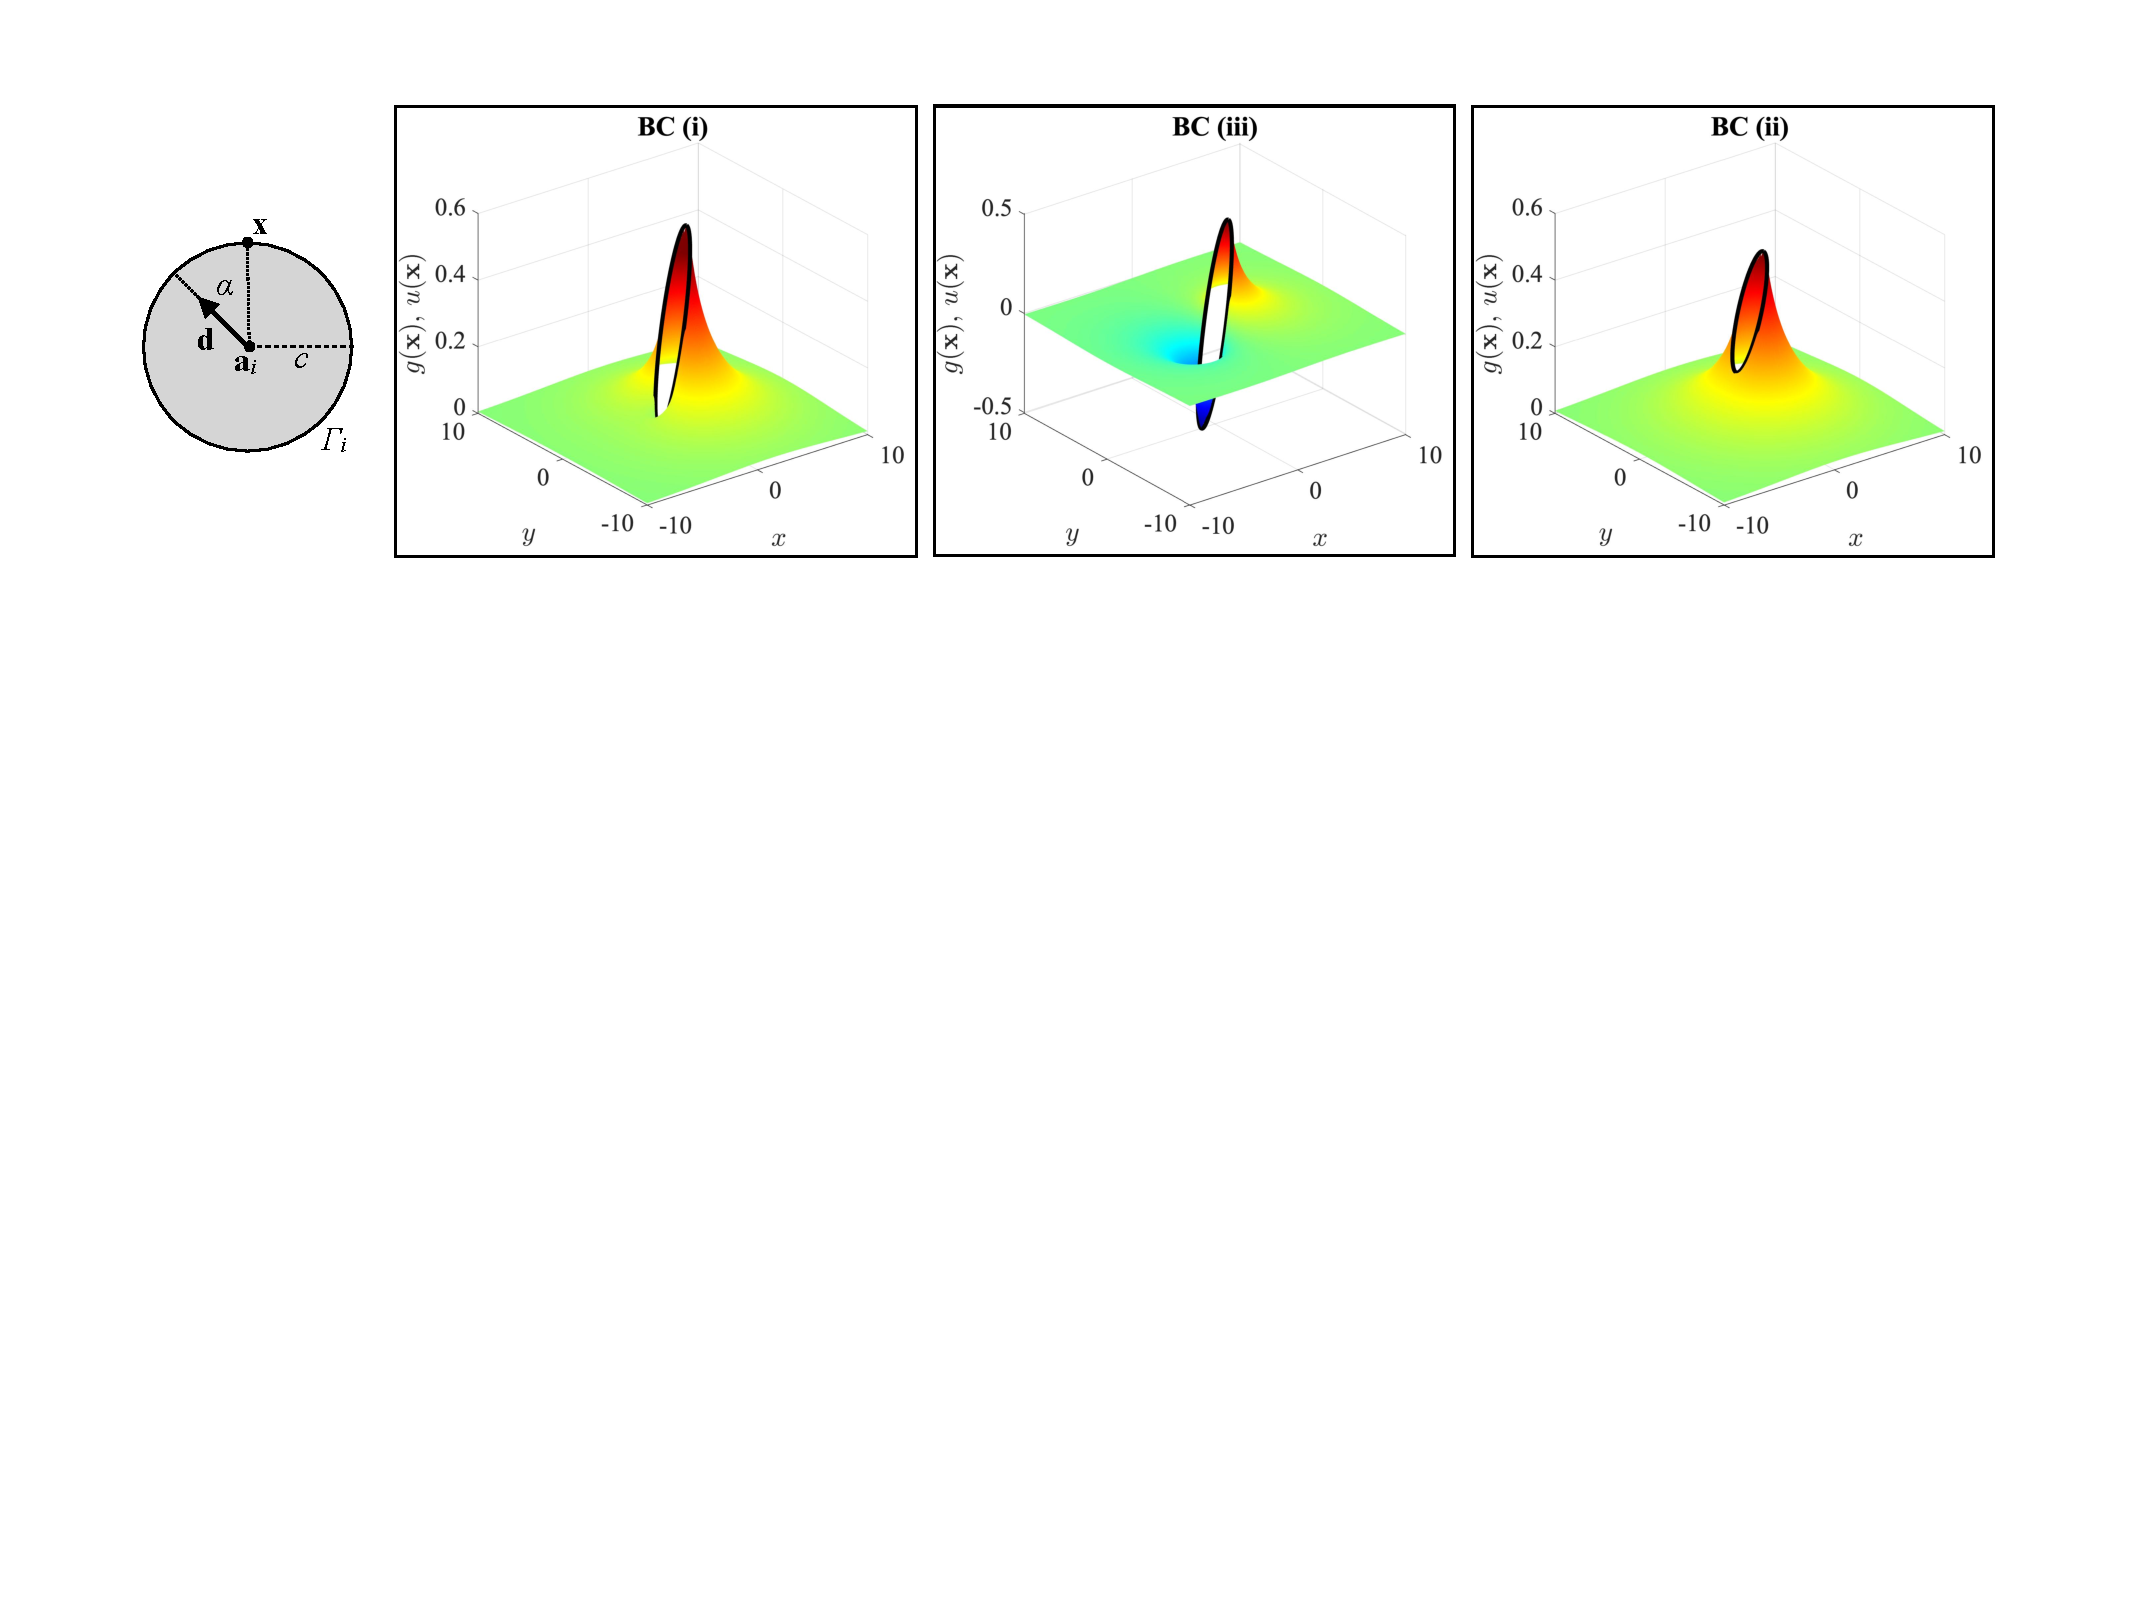
\includegraphics[width=\textwidth]{Figures/Figure0.pdf}
\end{center}
\begin{caption}{\label{fig:boundary_conditions} The leftmost diagram
  illustrates the particle $\Gamma_i$ with center $\aa_i$, radius $c$,
  and director $\dd$, along with the angle $\alpha$.
  The three rightmost panels plots show $g(\xx)$ and
  the respective solutions $u(\xx)$ of~\eqref{eq:SL} 
  for an isolated particle.}
\end{caption}
\end{figure}

%%%%%%%%%%%%%%%%%%%%%%%%%%%%%%%%%%%%%%%%%%%%%%%%%%%%%%%%%%%%%%%%%%%%%%%
\subsection{Boundary conditions and equilibrium configurations}
The boundary condition $g(\xx)$ in \eqref{eq:SLbc} defines the spatial
distribution of hydrophobicity and hydrophilicity.  Referring to Figure
\ref{fig:boundary_conditions}, we let
\begin{align}
  \label{eq:bc-type}
g(\xx) = a(b + \cos \alpha),\quad a = (\pi c(2b^2 + 1))^{-1/2},\quad \xx \in \Gamma_i,
\end{align}
where $\alpha$ is the angle between the vector $\xx - \aa_i$ and the
particle director $\dd_i = (\cos \theta_i, \sin \theta_i)$.  The scalar
$b$ shifts the periodic date up and down and the scalar $a$ normalizes
$g$ so that $\int_{\Gamma_i} g^2(\xx) \, \dif s = 1$. The side of the
particle where $\alpha = 0$ is called the tail and the side where
$\alpha = \pi$ is the head.

Based on the choice of $b$, the boundary condition (BC)
\eqref{eq:bc-type} can be classified into one of three categories: Type
I, amphiphile, $b = 1$, $g$ is positive on one side representing a
hydrocarbon-water interface, and is zero on the other representing an
apolar, hydrophilic region; Type II, asymmetric hydrophobe, $b = 2$, $g$
is positive on both sides but more so on one side; Type III, polar, $b =
0$, $g$ is positive on one side and negative on the other, representing
a water structure with positive/negative charge~\cite{MaRa76, Ma77}.

Figure~\ref{fig:relax} shows the steady state in a quiescent flow.
Three distinct phases emerge. For Type I, amphiphiles, the tail
interactions are attractive, and particles collectively form disjoint
bilayer components (Figure~\ref{fig:relax}(b)). We refer to this as the
``bilayer'' phase.


\begin{figure}[t!]
\begin{center}
  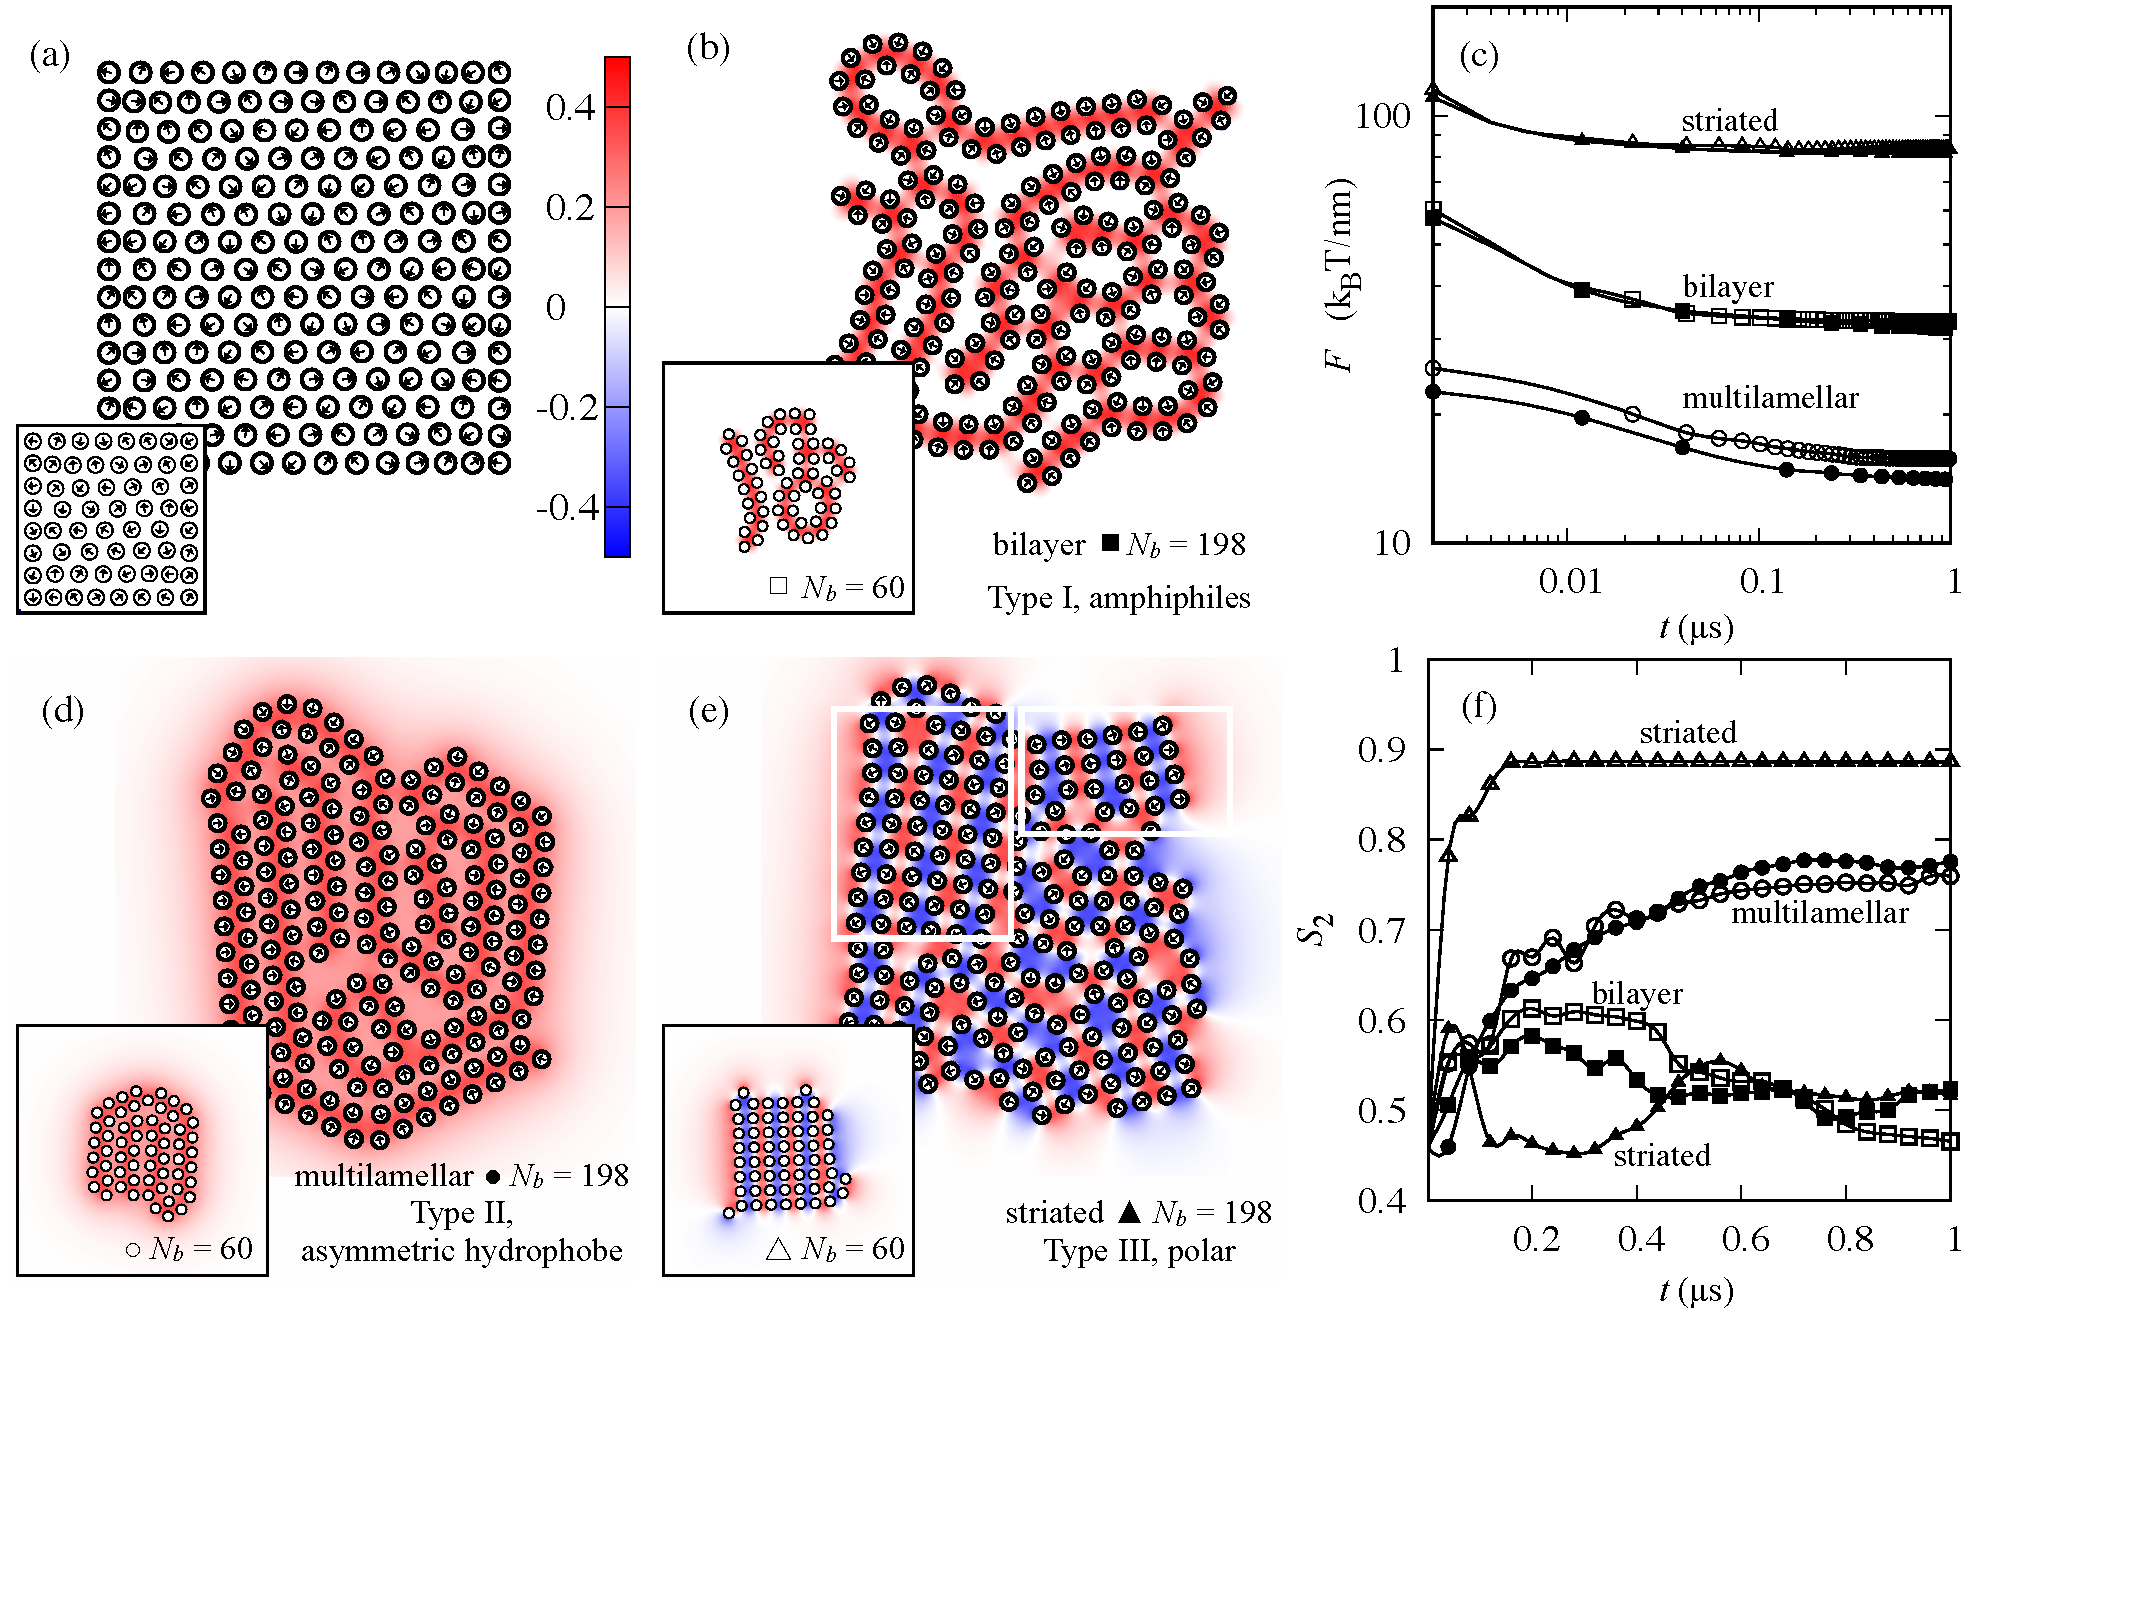
\includegraphics[width=\textwidth]{Figures/Figure1and2.pdf}
%  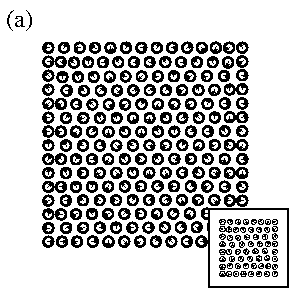
\includegraphics[height=0.3\textheight]{Nb198a_inset.pdf}
%  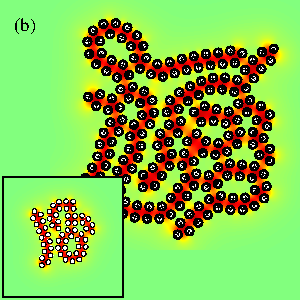
\includegraphics[height=0.3\textheight]{Nb198b_eta_inset.pdf}\\
%  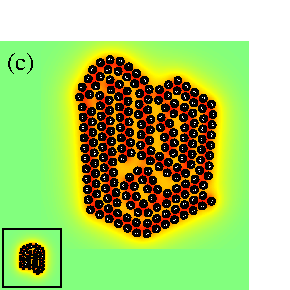
\includegraphics[height=0.3\textheight]{Nb198c_eta_inset.pdf}
%  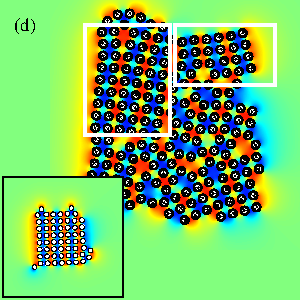
\includegraphics[height=0.3\textheight]{Nb198d_eta_inset.pdf}
\end{center}
\begin{caption}{\label{fig:relax}
  Panel (a) shows the $t = 0$, $N_b = 198$ particle configuration with
  random orientation and initially confined to a box. Panels (b), (d),
  (e) show bilayer, multilamellar, and striated phases composed of
  amphiphilic (Type I), asymmetric hydrophobe (Type II), and polar (Type
  III) JP, respectively. Panels (c) and (f) plot the free
  energies~\eqref{eq:free_energy} and alignment order
  parameter~\eqref{eq:S2} with respect to $t$. The open markers in panel
  (c) are for $N_b = 60$ and the solid markers are for $N_b = 198$ but
  normalized by $60/198$, showing that the energy approximately scales
  with the number of particles. Alignment in the striated phase is
  particle-number dependent; triangle markers, panel (f).}
\end{caption}
\end{figure}

For Type II, asymmetric hydrophobes, both sides of the JP are
hydrophobic but more so on the tail. Over short times, these particles
self-assemble into bilayers. But unlike for Type I JPs, the heads are
also hydrophobic and so over long times, the bilayers sort into a
``multilamellar'' phase. The number of layers depends on the number of
particles. Figure~\ref{fig:relax}(d), for example, shows a multilamellar
structure with four layers and one with two layers in the inset.
Onion-like dendrimersomes have previously been studied by molecular
dynamics simulations using an anisotropic pair
potential~\cite{C9NR05885K,HongCacciutoLuijtenGranick2008}.

Finally, Type III, bipolar JPs possess a head that repels the tail of
neighboring particles. These JP initially form chains with their
directors perpendicular to the length of the chain. The chains form
stria where the particles lie on a square grid and the orientations
alternate between layers (Figure~\ref{fig:relax}(e)). We refer to this
as the ``striated'' phase. 

See Section~\ref{sec:movie_description} in the [Supplementary Material]
for movies showing the transition of 60 JPs that are initialized
randomly (inset of Figure~\ref{fig:relax}(a)) to the steady state
configurations (inset of Figures~\ref{fig:relax}(b), (d), and (e)).


%\begin{figure}
%  \begin{center}
%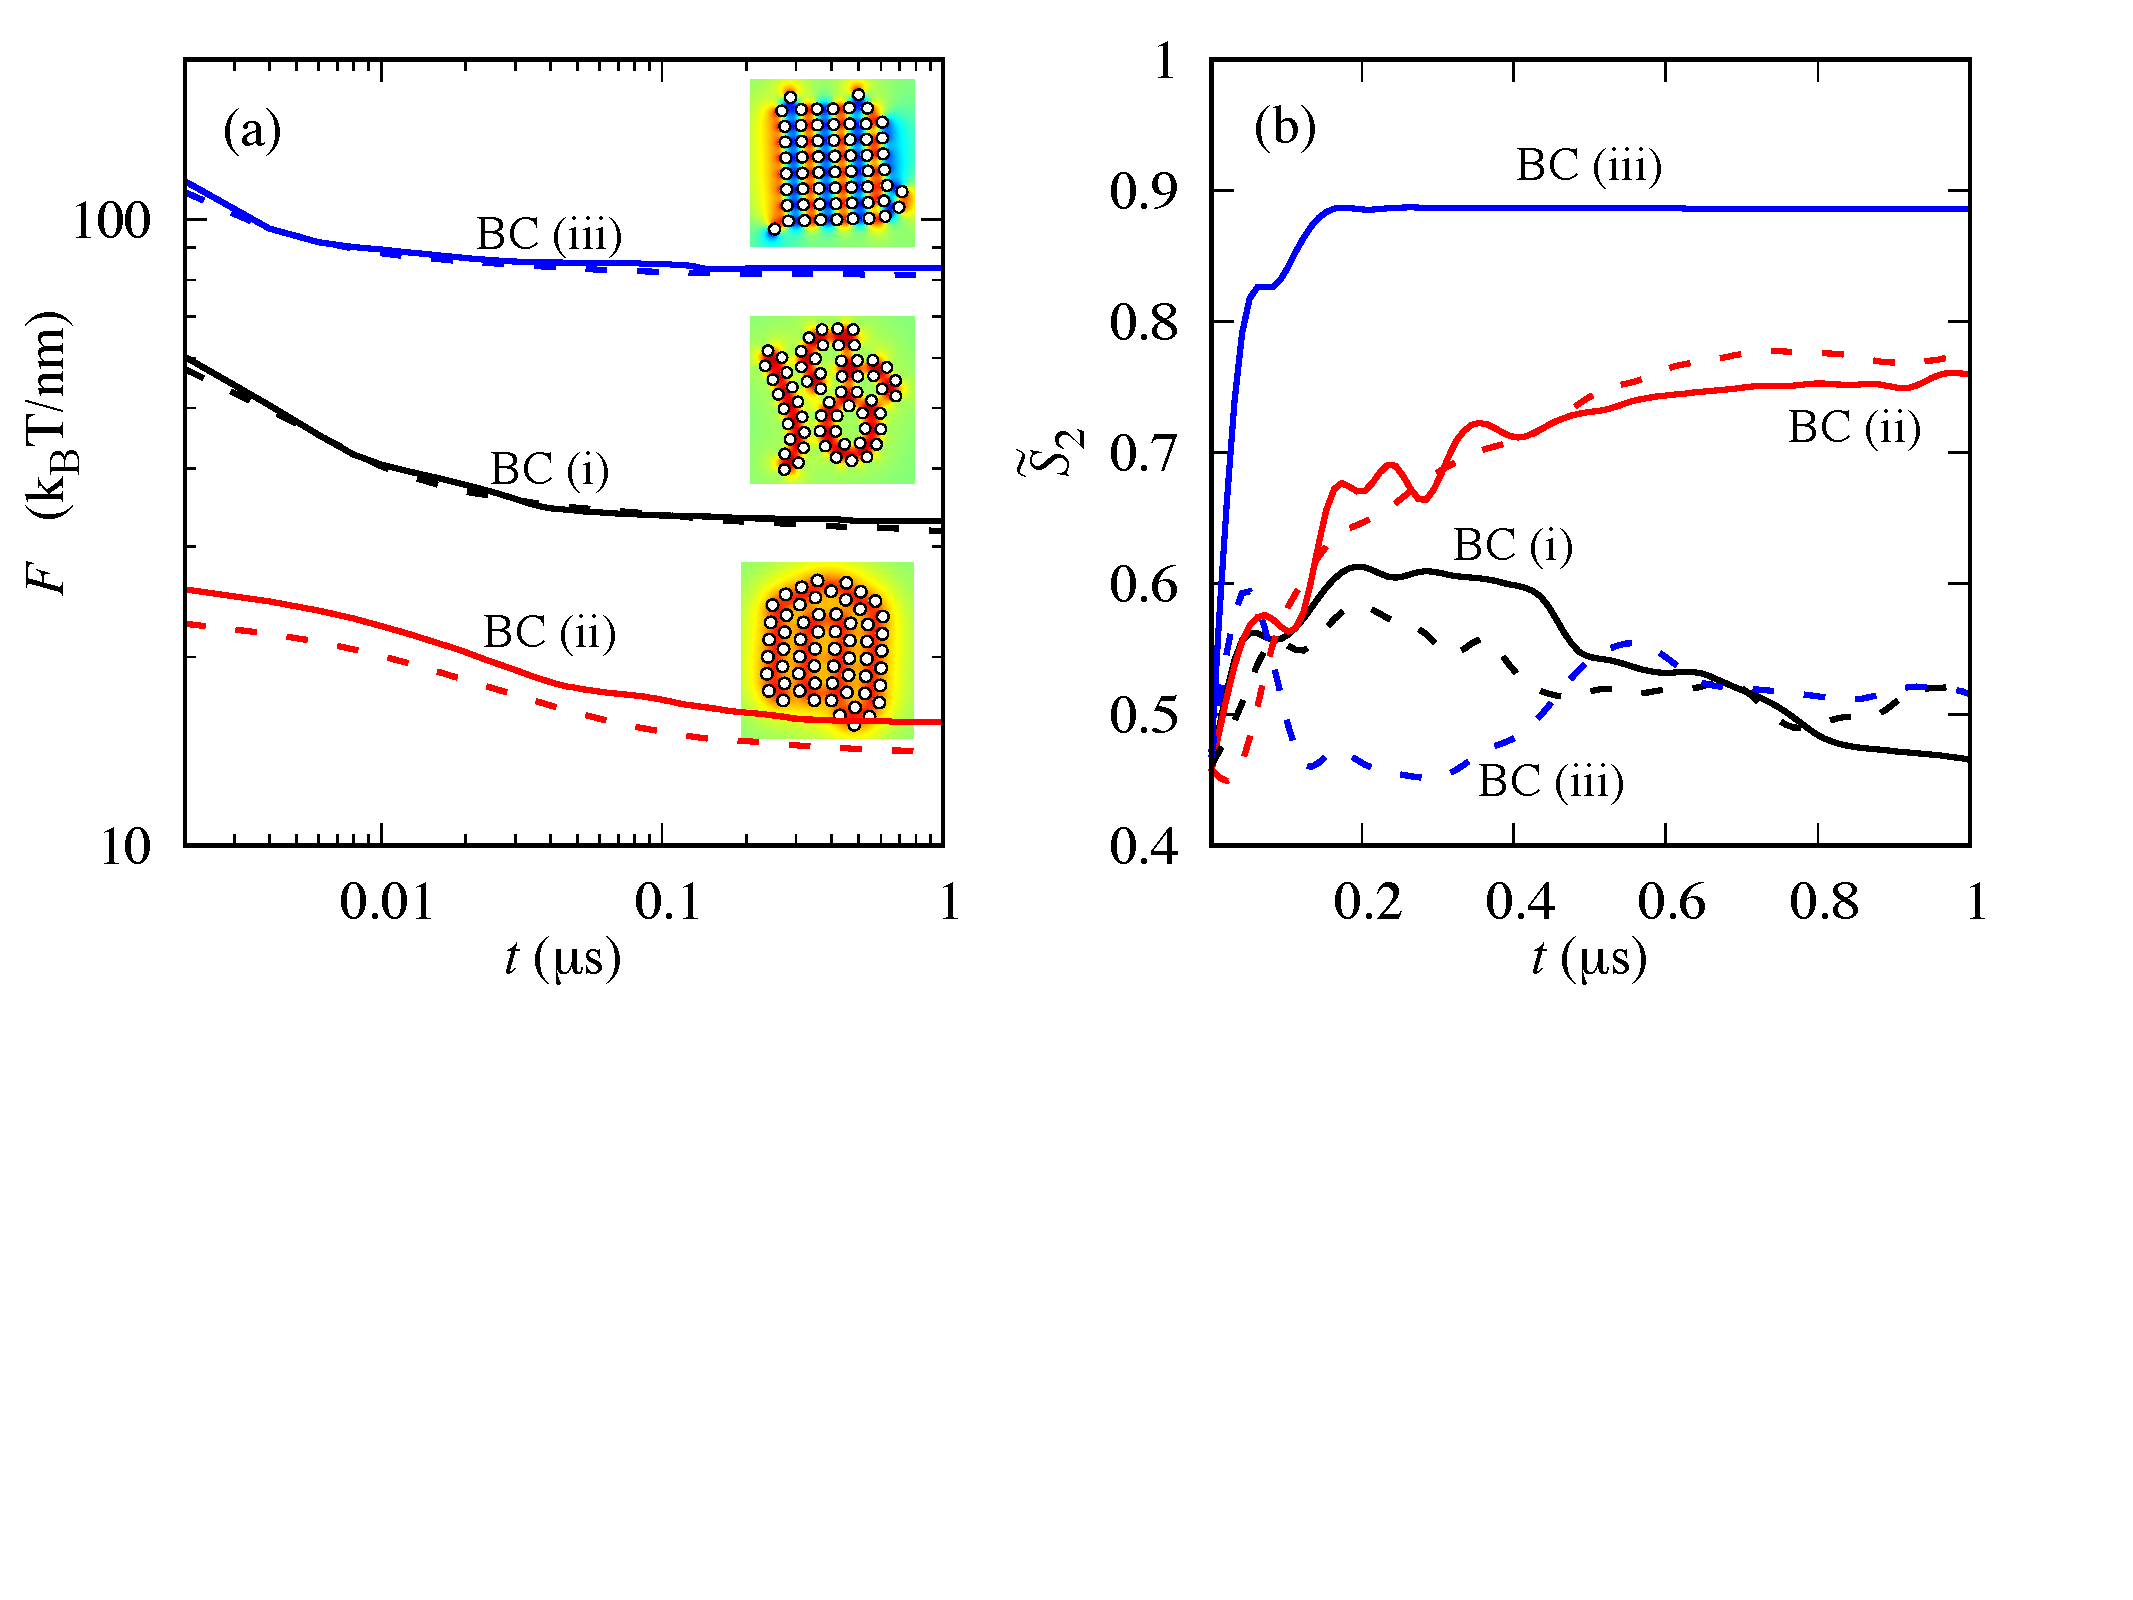
\includegraphics[width=1.0\textwidth]{Figures/Figure2.pdf}
%  \end{center}
%  \vspace{-20pt}
%  \caption{\label{fig:relax_energy}
%  Panel (a) shows that the free energy~\eqref{eq:free_energy} decreases
%  in the mobility problem formulation. The initial energies are for the
%  configuration in Figure~\ref{fig:relax}(a) and the final energies are
%  for the near-equilibrium configurations shown in
%  Figures~\ref{fig:relax}(b)--(d). The solid curves are the energies for
%  the $N_b=60$ cases and the dashed curves are the energies for the $N_b
%  = 198$ cases normalized by $60/198$, showing that the energy
%  approximately scales with the number of particles.  Panel (b) shows
%  the orientational parameters $\tilde{S}_2$ for all 6 relaxation runs.
%  The curve styles are identical those in panel (a). The
%  near-equilibrium configurations depend on the initial configurations
%  and the results show that for both $N_b=60$ and $N_b=198$ cases,
%  bilayer and multi-lamellar configurations have similar trends in
%  orientational parameters. The results of the striated configuration,
%  however, depend on the initial geometrical setup.}
%\end{figure}

\section{Measuring deformation}
\label{sec:measuring_deformation}
To quantify the hydrodynamics of JP phases, we use the free energy $F$,
a strain parameter $E$, and a scalar order parameters $S_{2}$ for
alignment. First we simplify the form of the free
energy~\eqref{eq:free_energy}. Using integration by parts
and~\eqref{eq:SL}, we obtain
\begin{equation}
\label{eq:free_energy2}
F = -\gamma
\int_{\partial \Omega} \rho g \nabla u \cdot \nnu \,\dif s
+ \frac{M}{2}
\sum_{j \neq i} 
P\left(\frac{|\aa_i - \aa_j|-2c}{\rho_0}\right).
\end{equation}
%
Here, we have substituted $g$ for $u$ since the boundary values are
given. However, evaluating $\nabla u \cdot \nnu$ on $\partial \Omega$
based on~\eqref{eq:SL_BIE} involves calculating a gradient of a
double-layer potential which has a well-known obstacle in numerical
implementation. Appendix~\ref{sec:appendix} describes how we overcome
this obstacle.

Figure~\ref{fig:relax}(c) tracks the free energy profiles for all
relaxation runs. In quiescent background flow, the energies are
decreasing with respect to $t$ showing time stepping correctly accounts
for viscous dissipation. Furthermore, the normalized energy plots
provide evidence that the free energy per particle with specified
boundary condition is independent of the total particle number $(N_b)$.

To measure positional order, we introduce the strain parameter, 
\begin{equation}
\label{eq:SP}
E = \frac{1}{N_b} \sum_{i=1}^{N_b}
\left\|\tfrac{1}{2}(\mathsf{F}_i^T \mathsf{F}_i - I)\right\|,
\end{equation}
where $\mathsf{F}_i$ is an approximate deformation gradient and $\|
\cdot \|$ is the Frobenius norm. The Green-Lagrange strain tensor
$\tfrac{1}{2}(\mathsf{F}_i^T \mathsf{F}_i - I)$ measures departure of
fluid deformations from a rigid body motion. To define $\mathsf{F}_i$,
we solve the overdetermined system 
\begin{align}
\aa_j(t) - \aa_i(t) = \mathsf{F}_i(\aa_j(0) - \aa_i(0)),\quad j =
  1,\ldots, N_b,
\end{align}
for $\mathsf{F}_i$ by weighted least squares. That way, if the particle
positions are given by a map $\ff(\aa_i(0),t) = \aa_i(t)$, then
$\mathsf{F}_i \approx \nabla \ff(\aa_i(0),t)$. The weights $w_i =
\exp(-\|\aa_j(0) - \aa_i(0)\|/4c)$ with particle radius $c$ ensure that
the linear approximation holds for particles near $\aa_i$.

Finally, we use the scalar order parameter $S_2$ to quantify the
orientational order~\cite{Selinger2016}:
\begin{equation}
  \label{eq:S2}
S_2 = \frac{1}{N_b} \sum_{i=1}^{N_b} \frac{1}{2}(3\cos^2(\theta_i - \bar \theta) - 1).
\end{equation}
Here $\bar \theta_i$ is a circular mean defined as the orientation of
the principal eigenvector of the matrix $\sum_{j} \dd_j\dd_j^\top$ where
$j$ runs over the particles whose centers lie with $4c$ of that of
particle $i$. Defined as such, $S_2$ lies in the range $-1/2 \le S_2 \le
1$ with a value $S_2 = 1$ indicating perfect alignment between particles
while $S_2=-1/2$ indicating isotropic alignment locally. The cutoff
distance $4c$ was chosen empirically so that the average includes
nearest neighbors but excludes next nearest neighbors.

In Figure~\ref{fig:relax}(f), the multilamellar phase is highly ordered
whereas the bilayer phase is somewhat disordered because it consists of
several components forming isolated bilayers, micelles, and vesicles
(Figure~\ref{fig:relax}(b)).

The striated phase order admits more than one pattern depending on the
number of particles (Figure~\ref{fig:relax}(f), triangles). When the
number of particles is fewer, there is only a single pattern where the
directors are more or less parallel and alternate directions
(Figure~\ref{fig:relax}(e), inset). Larger number of particles results
in multiple alignment patterns: the alternating sign pattern as in the
small particle number case (Figure~\ref{fig:relax}(e), top right
rectangle) and an `X'-shaped alignment (Figure~\ref{fig:relax}(e), top
left rectangle).

%%%%%%%

\section{Results and Discussion}
\label{sec:results}
\begin{figure}[t]
\begin{center}
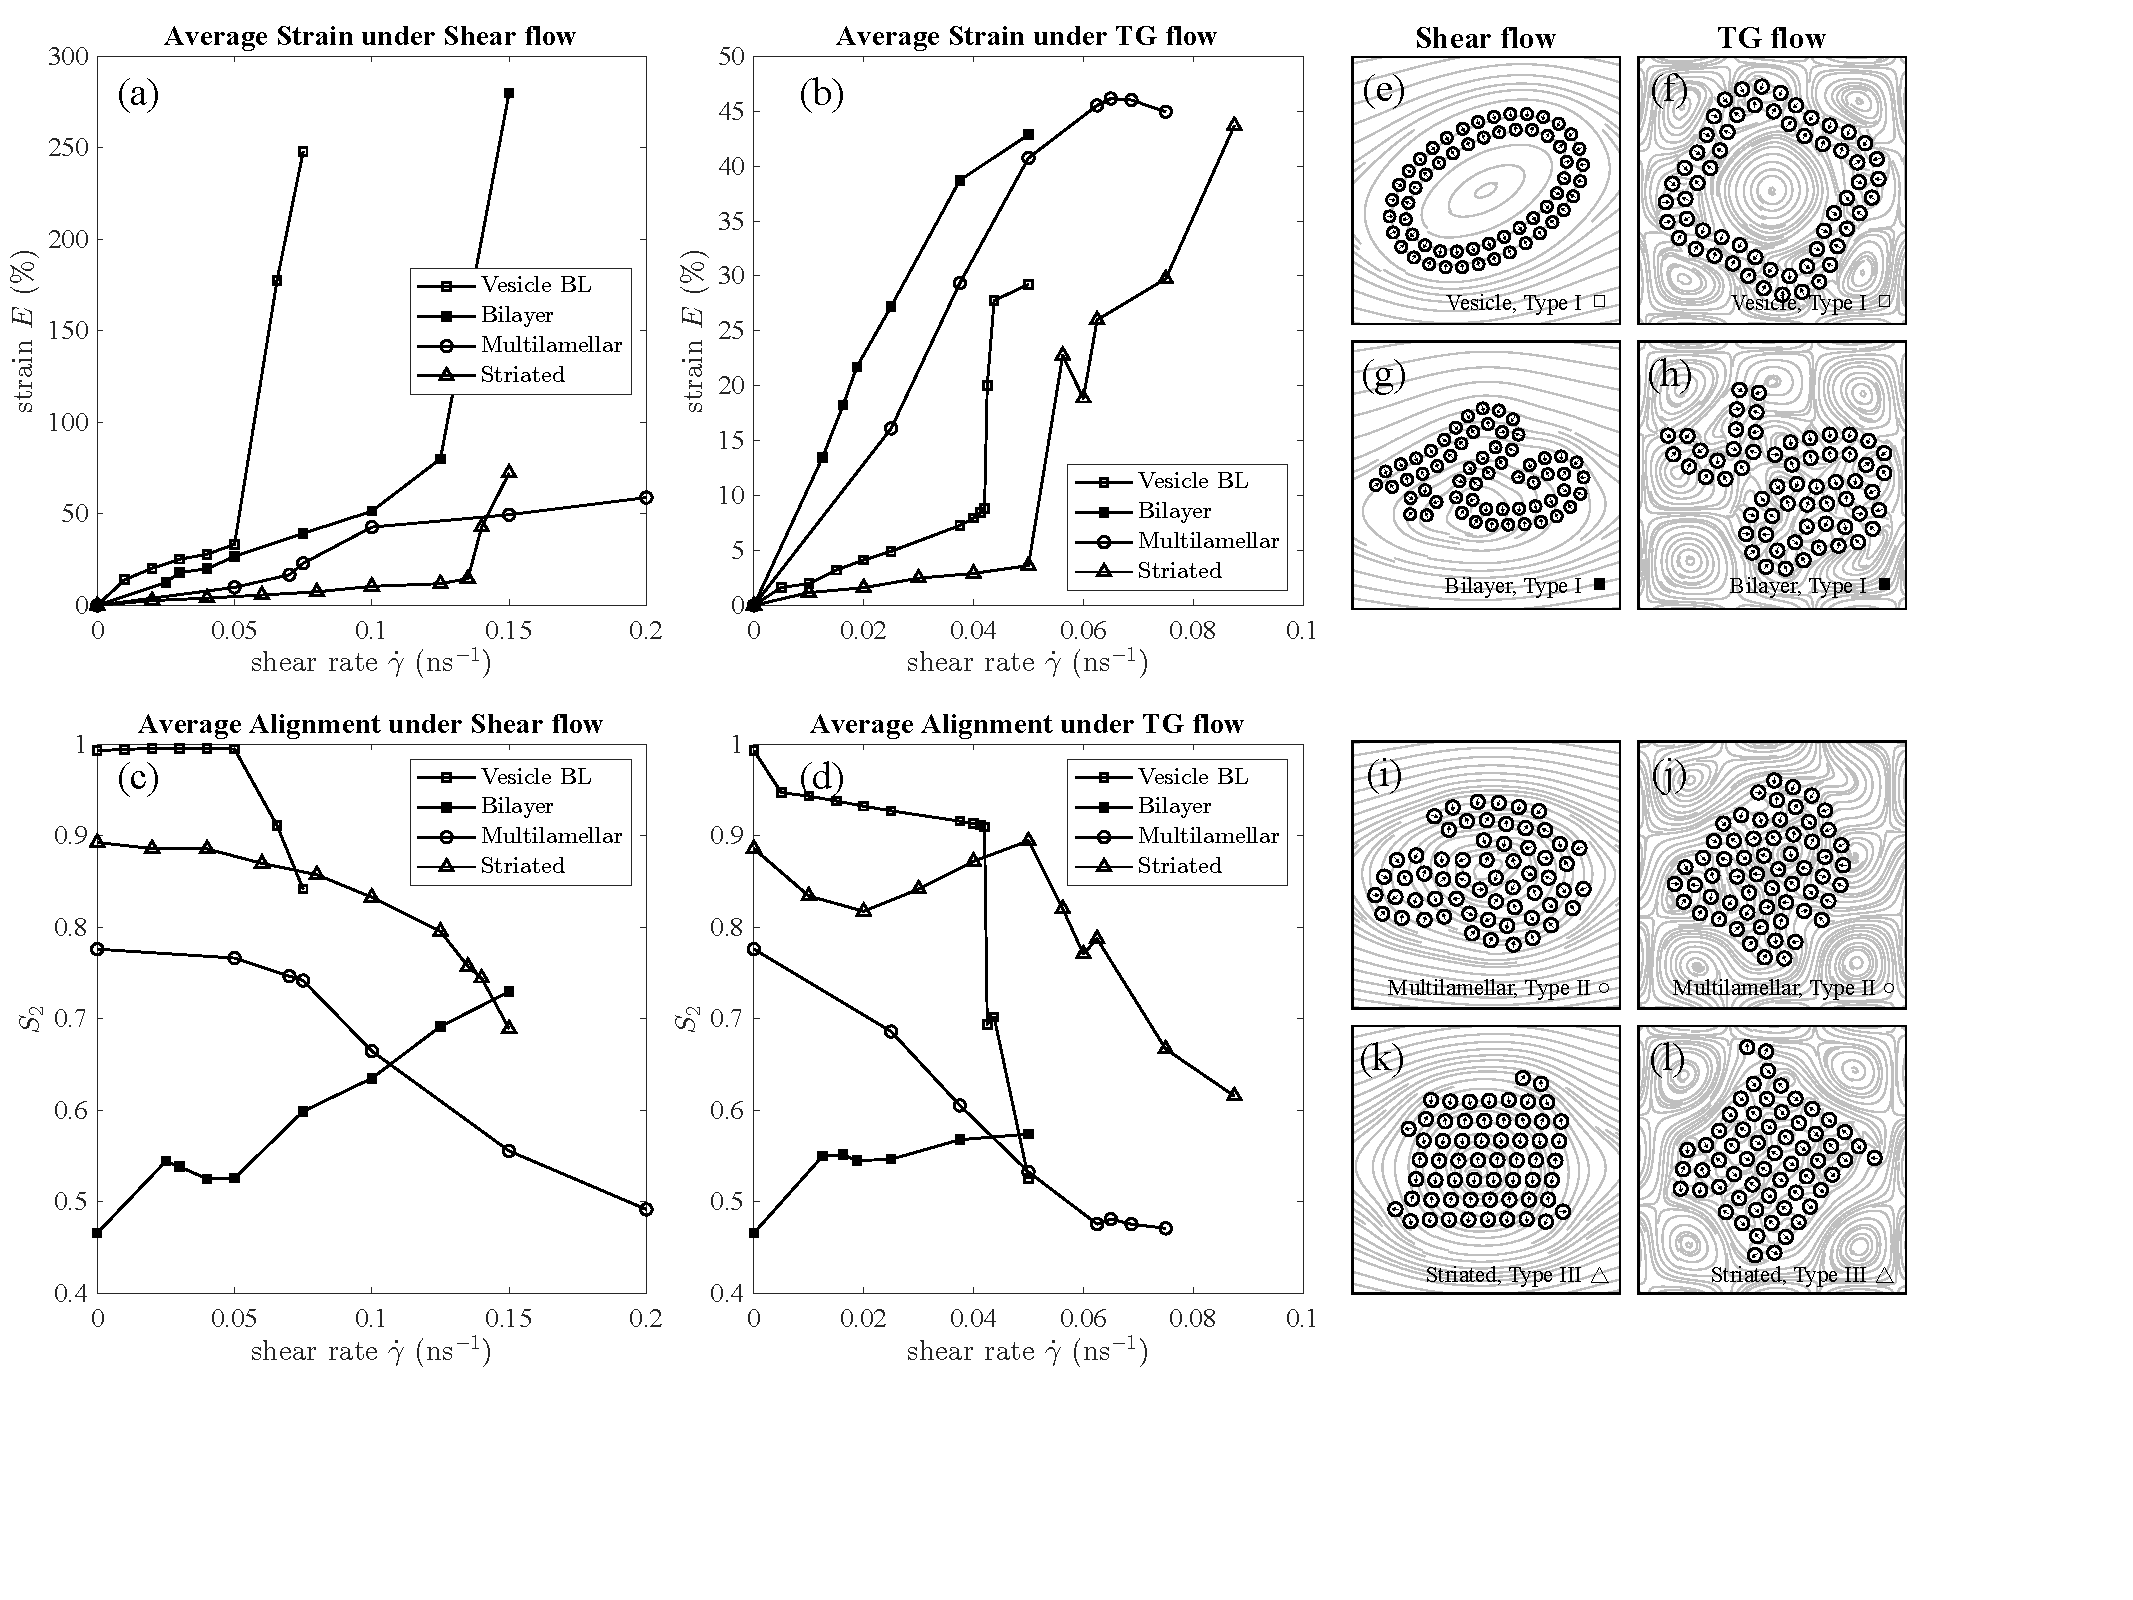
\includegraphics[width=\textwidth]{S2ESummary.pdf}
\end{center}
\caption{\label{fig:s2esummary}
  Panel (a)--(b) show the average strain increase for bilayer, vesicle
  BL, multilamellar, and striated JP structures under a shear flow and a
  TG flow, respectively. Panel (c)--(d) show the average alignment of
  four JP structures under a shear flow and a TG flow, respectively.
  Each snapshot of panels (e)--(l) contains the configurations of the JP
  structure without ruptures using a specific type of boundary condition
  and the background curves indicate the velocity streamlines.}
\end{figure}
%
We subject the Type I, II, and III JP phases to background flows and
measure their material response. The background flows are a shear flow
\begin{equation}
\label{eq:sh_flow}
\uu_\infty^{\text{sh}}(\xx) = 
\dot\gamma (\ee_y \cdot \mathbf{x})\ee_x,
\end{equation}
and a Taylor-Green (TG) flow
\begin{equation}
\label{eq:tg_flow}
\uu_\infty^{\text{TG}}(\xx) = 
\lambda \dot \gamma \left(
-\cos(\ee_x\cdot\xx/\lambda)\sin(\ee_y\cdot\xx/\lambda)\ee_x
+\sin(\ee_x\cdot\xx/\lambda)\cos(\ee_y\cdot\xx/\lambda)\ee_y\right),
\end{equation}
where the orthonormal vectors $\ee_x$ and $\ee_y$ are the horizontal and
vertical directions, respectively. The shear flow replicates the motion
of a fluid between two parallel, moving plates excluding wall effects.
In TG flow, $\lambda$ controls the size of the $2\pi \lambda \times 2\pi
\lambda$ TG cells. Throughout this section, we use $\lambda = 2$ nm so that the JP
phases occupy about nine cells.

In both cases, $\dot \gamma$ is the shear rate. The flow rate $\lambda
\dot \gamma$ is chosen so that~\eqref{eq:tg_flow} has the same rate of
viscous dissipation per area as for~\eqref{eq:sh_flow}. In other words,
$\int_{A} \frac{1}{2}\mu |\nabla \uu + \nabla \uu^T|^2 \,\dif A$ is the
same for $\uu = \uu_{\infty}^{\text{sh}}$ as for $\uu =
\uu_{\infty}^{\text{TG}}$ when integrated over a TG cell $A$. 

To obtain a range for $\dot \gamma$, consider the capillary number 
\begin{equation}
\label{eq:capillary}
C_a = \frac{\mu \dot \gamma R^3}{\kappa}
\end{equation}
where $R = 10$~nm and $\kappa = 20\;\kbt$ are the characteristic phase
sample radius and bending rigidity, respectively. That is, $\kappa$
gives the elastic stress for restoring the phase-sample shape. Shear
stress overcomes elastic stress when $C_a > 1$ and this yields $\dot
\gamma > 2 \cdot 10^{-2}$ ns$^{-1} = 2 \cdot 10^6$~s. Thus our values
for $\dot \gamma$ range between $0$ ns$^{-1}$ corresponding to quiescent
flow up to $0.2$~ns$^{-1}$ capable of rupturing the sample. Such shear
rates are compatible with molecular dynamics simulation
\cite{Brandner2019}, those for large unilamellar vesicles (LUV),
\cite{Bernard2005ShearinducedPA}, and shearing in blood capillary
vessels \cite{Cho2011} where shear rates range over 100--2000 s$^{-1}$.

For initial data, note that the steady-state Type I amphiphiles phase
consists of a number of disjoint bilayer components
(Figure~\ref{fig:relax}(b)). To also have a single-component Type I
phase, we reinitialize the data to have a ring-shaped vesicle bilayer.
This phase is distinguished from ``bilayer'' by ``vesicle BL'' in the
figures. For the same number of JP, the vesicle bilayer has lower free
steady-state energy ($F = 24.6 \;\kbt$ nm$^{-1}$) than the disordered
bilayer phase ($F = 27.2 \;\kbt$ nm$^{-1}$). Since the simulations are
for two dimensions, multiplying $F$ by a length gives the energy of a
transversely invariant, three-dimensional phase.

The simulation setup consists of placing each of the phases in either a
shear or TG background flow and then solving for the particle
trajectories in time. In each setup, we solved for $500$ time steps with
$\Delta t = 2$~ns, yielding time courses for $t \in [0, T]$, $T =
1$~$\upmu$s. We then post-process the trajectories.

Figure~\ref{fig:s2esummary}(e)--(l) show the typical streamlines for JP
phases in background flow. Although the plots only show the region near
the JPs, the fluid velocity $\uu$ and order parameter $u$ are accounted
for in all of $\mathbb{R}^2$. Moreover, $\uu$ satisfies the rigid
boundary condition at every JP-fluid interface i.e., the particles
interact with the local flow field and are not merely carried by
background flow. See Section~\ref{sec:movie_description} in the
[Supplementary Material] for movies showing the dynamics of the JP
suspensions in Figure~\ref{fig:s2esummary}.

Figures~\ref{fig:ulshraw}--\ref{fig:sttgraw} in the [Supplementary
Material] contain the fully-resolved time courses for the free energy
$F$, alignment order $S_2$, and strain $E$. The eight setups correspond
to the four JP phases---bilayer, vesicle BL, multilamellar, and
striated---and two background flows---shear and TG, and the data are
plotted with the same vertical and horizontal axes to facilitate
comparisons between simulation setups. Each setup considers a range of
shear rates $\dot \gamma$ in the interval $[0, 0.2]$ ns$^{-1}$.

The fully-resolved time courses in
Figures~\ref{fig:ulshraw}--\ref{fig:sttgraw} in the [Supplementary
Material] contain significant oscillations due to the particle-based
formulation and tumbling inherent to the background flows. To extract
meaningful data, we further post-process the $F$, $S_2$, $E$ curves by
taking their time average over the interval $t \in [0, T]$. 

\subsection{Strain and alignment}
\label{sec:strain-alignment}
The plots reveal highly distinct material responses from each phase.
Figures~\ref{fig:s2esummary}(a) and (b) show the time-averaged strain
$\frac{1}{T}\int_0^T E \,\dif t$ over a broad range of shear rates.
Strain $E$ measures the non-rigid-body deformation relative to the
initial state and expectedly increases with shear rate. The greatest
increase occurs with the Type I amphiphiles, suggesting that this phase
has the lowest elastic modulus (squares). In comparison, the striated
phase consisting of Type III polar JP is basically rigid (triangles).

Figures~\ref{fig:s2esummary}(c) and (d) plot the time-averaged alignment
order $S_2$. The vesicle and striated phases possess the greatest
alignment order and, for the most part, $S_2$ decreases with increases
in shear rate. But there is an exception. The Type I bilayer phase
alignment order actually increases under both shear and TG flows (solid
squares). This suggests that the mixing action of background flow has
the effect of moving the disordered bilayer phase out of a local
equilibrium and into a state with greater order. This surprising
increase, brought about by combining previously broken bilayer end caps,
is accompanied by a slight decrease in free energy
(Figure~\ref{fig:fsummary}(a), solid squares).

The sudden jumps in Figures~\ref{fig:s2esummary}(a) and (b) and
commensurate drops in panels (c) and (d) indicate the existence of a
critical shear rate $\dot\gamma_*$. This means that for $\dot\gamma < \dot\gamma_*$,
the JP phase remains intact while for $\dot\gamma > \dot\gamma_*$, the phase
ruptures. For example, the vesicle BL phase has $\dot\gamma_*$ approximately
$0.05$ ns$^{-1}$ under shear flow and TG flow. However, the critical
shear rate is flow-pattern dependent because the striated phase has
$\dot\gamma_* = 0.14$ ns$^{-1}$ under shear flow while $\dot\gamma_* = 0.05$
ns$^{-1}$ under TG flow. Due to variable stress distribution, the
critical shear rate in TG flow likely depends on the cell size parameter
$\lambda$. The disordered bilayer phase does not really possess a
critical shear rate because it already consists of several, disjoint
components. The jump in Figure~\ref{fig:s2esummary}(a) (solid squares)
simply corresponds to disjoint components drifting apart in the shear
flow. The Type II multilamellar phase did not rupture for any of the
shear rates considered.

\begin{figure}[t]
\begin{center}
\includegraphics[width=\textwidth]{FSummary.pdf}
\end{center}
\caption{\label{fig:fsummary}
  The change of average free energy versus shear rates for shear flow
  and TG flow simulation results are plotted in panels (a)-(b). Panel
  (c) contains quadratic fits to the change in free energy as a function
  of displacement in interparticle distance from equilibrium.}
\end{figure}

%%%%%%%%%%%%%%%%%%%%%%%%%%%%%%%%%%%%%%%%%%%%%%%%%%%%%%%%%%%%%%%%%%%%%%%
\subsection{Free energy}
\label{sec:free-energy}
Figure~\ref{fig:fsummary} plots the time-averaged relative free energy
$\frac{1}{T}\int_0^T (F - F_0) \,\dif t$ where $F_0$
is~\eqref{eq:free_energy2} at $t = 0$. The greatest increase occurs with
the Type II multilamellar phase, with the other phases showing a
moderate change in a few \KBT\,nm$^{-1}$.

Figure~\ref{fig:fsummary}(c) plots the free energy against the
displacement $x = c E$ representing the change in mean interparticle
displacement from equilibrium; $c = 1.25$~nm is the particle radius.
The energies in Figure~\ref{fig:fsummary}(c) are essentially quadratic
in $x$ suggesting that the interactions are harmonic locally around
equilibrium. The harmonic bond strength is strongest between polar JP,
and greater by a factor of two and five than that for asymmetric
hydrophobes and amphiphiles, respectively. This makes sense when
considering that the free energy of the steady-state striated phase is
also greatest (Figure~\ref{fig:relax}(c), around 85 \KBT\;nm$^{-1}$).
However, the bond strength in the multilamellar phase comes in second,
despite having least steady-state free energy (around
15~\KBT\;nm$^{-1}$). The data point to the fact that the binding
properties do not merely scale with free energy, but also involve the
details of the interface's hydrophobicity which are tuned
by~\eqref{eq:bc-type} in our model.

\begin{figure}[t]
\begin{center}
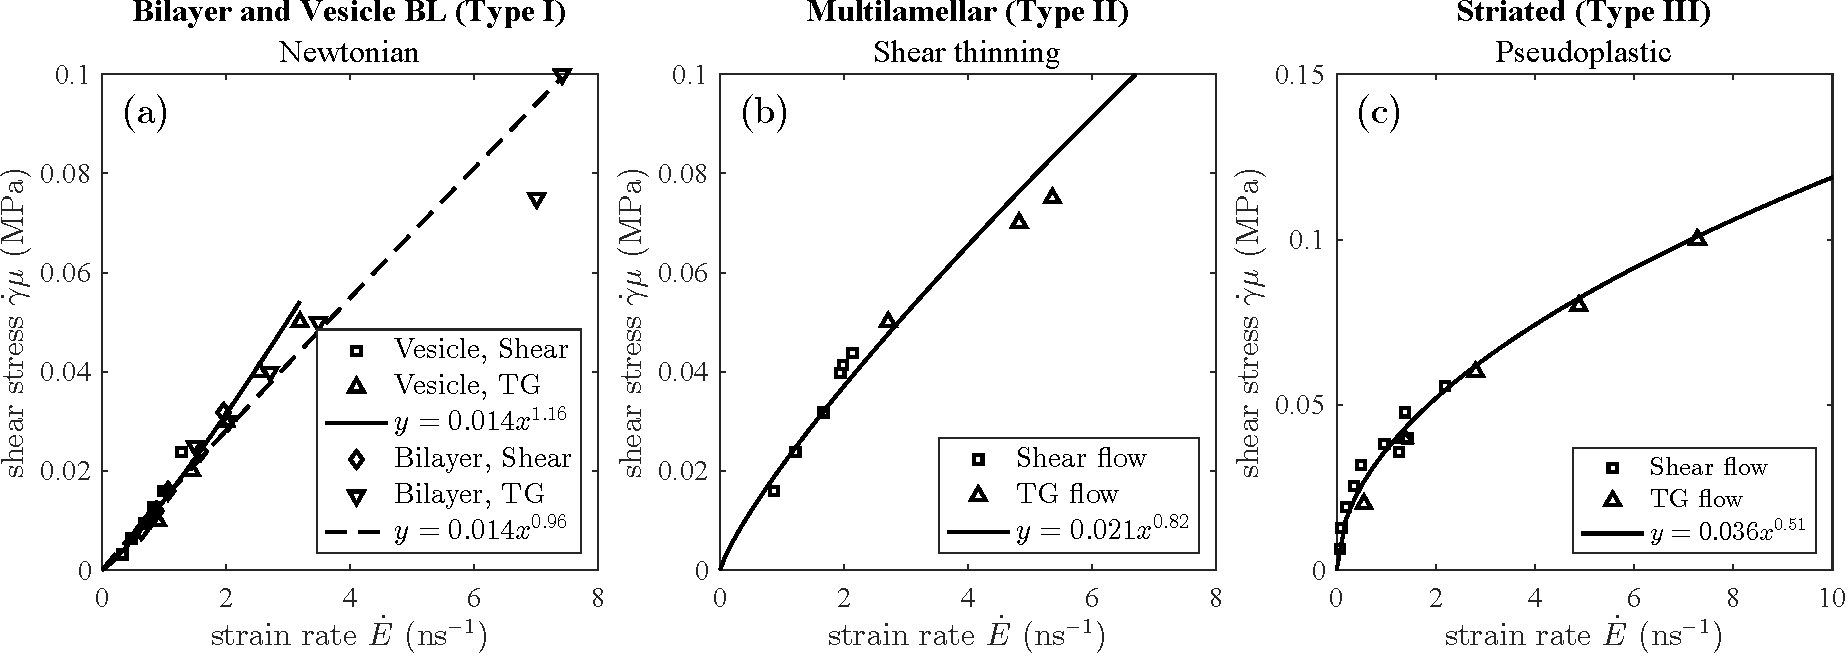
\includegraphics[width=\textwidth]{RheologySummary.pdf}
\end{center}
\caption{\label{fig:rheologysummary} Rheology of Type I, II, and III
  phases. Panel (a) shows that bilayer phases behave as a Newtonian
  fluid. Panel (b) provides that the multilamellar phase shows a near
  shear thinning behaviour. A pseudoplastic behaviour of deformation in
  striated phases is shown in panel (c).}
\end{figure}

%%%%%%%%%%%%%%%%%%%%%%%%%%%%%%%%%%%%%%%%%%%%%%%%%%%%%%%%%%%%%%%%%%%%%%%
\subsection{Rheology}
\label{sec:rheology}
So far, we have considered static material properties, namely constant
strains maintained by an external force provided by background flow.
Now we consider dynamic material properties. Specifically, we look at
the strain rate 
\begin{equation}
\label{eq:strainrate}
\dot E = \left(\frac{1}{T} \int_0^T \left|\frac{dE}{dt}\right|^2 \, \dif t \right)^{1/2}.
\end{equation}
The reason for defining $\dot E$ in this way is that the shear flow
$\uu_{\infty}^{\text{sh}}$ simulations correspond to a complex fluid
within a drag plate rheometer where the shear stress is set by $\mu
\dot\gamma$ and the observed, sample shear rate is $\dot E$. The
definitions carry over to the TG flow case directly. Also, as a
practical consideration, the rotation of non-isotropic JP phases in the
background flow leads to oscillation in the strain time courses making
systematic fitting challenging (see [Supplementary Material]
Figures~\ref{fig:ulshraw}--\ref{fig:sttgraw}). The integral
in~\eqref{eq:strainrate} averages out these oscillations and gives
physically meaningful values.

The shear stress-strain rate data are excellently fit by power laws.
Figures~\ref{fig:rheologysummary}(a)--(c) show the data for Type I, Type
II and Type III JPs, respectively, under both shear flow (squares) and
TG flow (triangles). The bilayer phases consisting of Type I JPs are
basically Newtonian with viscosity $0.014$ MPa\;$\upmu$s $= 14$ mPa\;s,
about 14 times the viscosity of water at room temperature
(Figures~\ref{fig:rheologysummary}(a), dashed curve). The vesicle
bilayer phase is slightly shear thickening
(Figure~\ref{fig:rheologysummary}(a), solid curve). Similar shear
thickening behaviors are found in continuum vesicle
models~\cite{rah-vee-bir2010,NaitOuhra2019RheologyOA}.
The multilamellar phase consisting of
Type II JPs is somewhat shear thinning, but its viscosity is larger than
for Type I. Finally, the striated phase is strongly shear-thinning. This
further explains the rigid-like behavior of the striated phase found in
the strain, shear-rate relationships from
Figures~\ref{fig:s2esummary}(a) and (b) (triangles).

\begin{figure}[t]
\begin{center}
  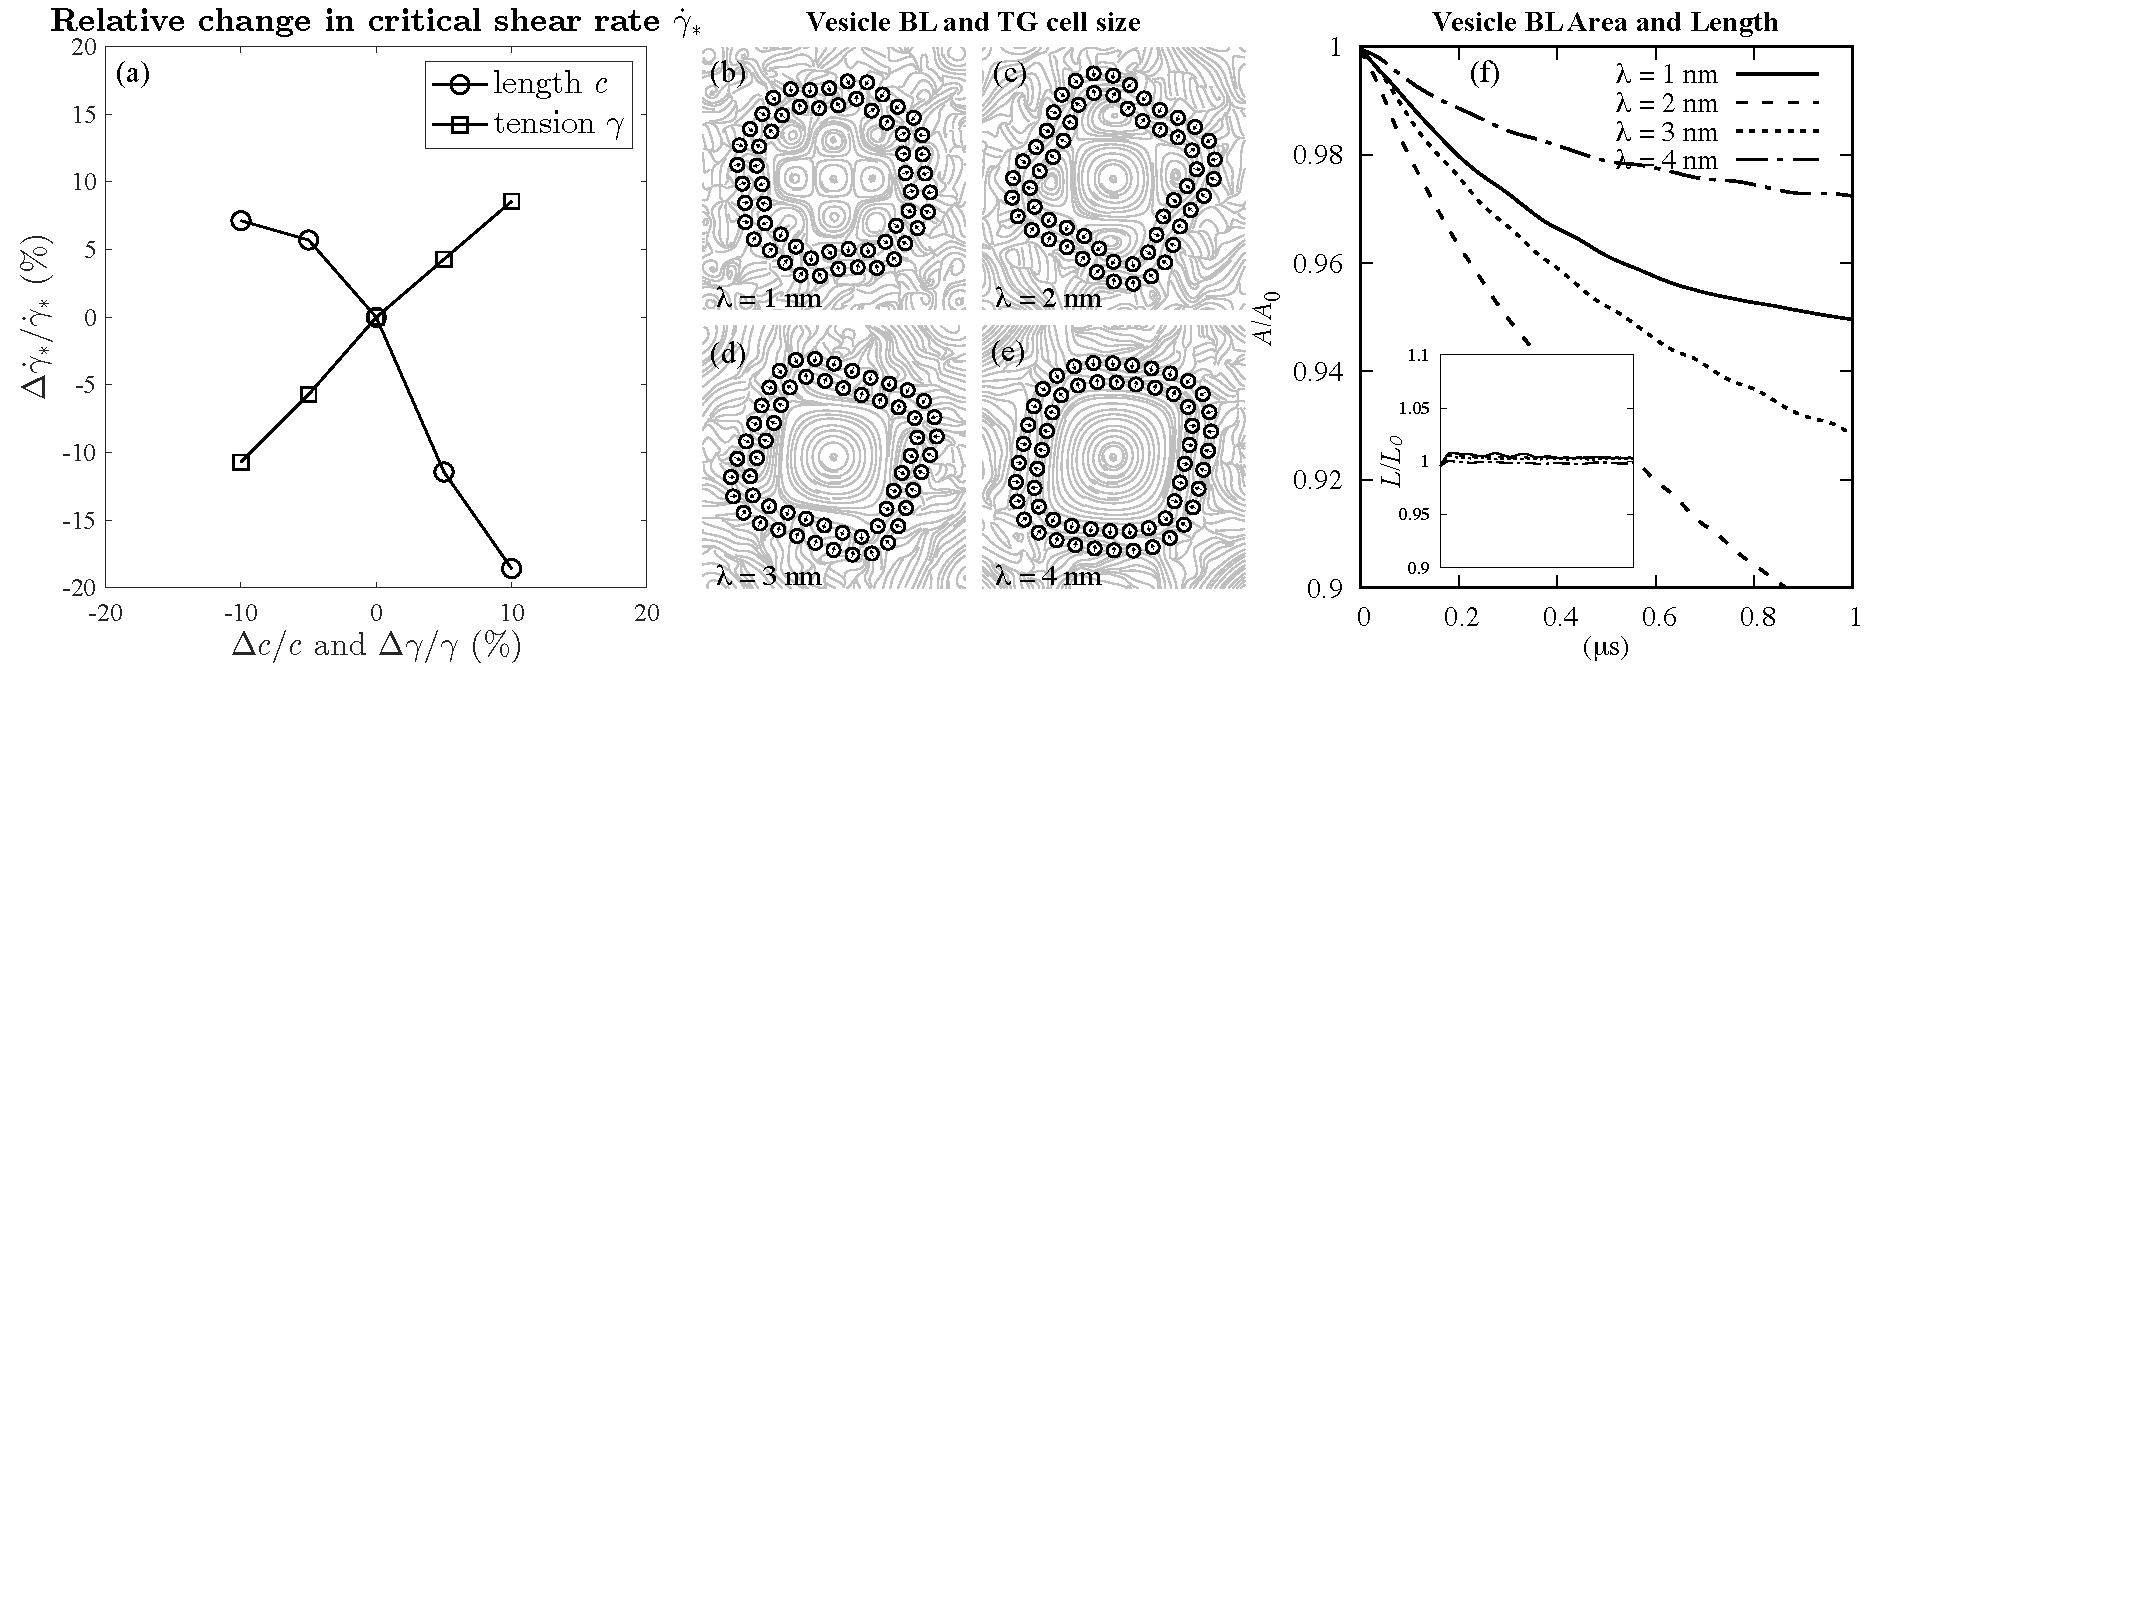
\includegraphics[width=\textwidth]{critical_shear_and_cell_size.pdf}
\end{center}
\caption{\label{fig:PramChange}
In panel (a), the relative change in $\dot \gamma_*$ is linear in the
  relative change of the tension parameters $\gamma$ and $M$ with slope
  $1$. Additionally, the relative change in $\dot \gamma_*$ has slope
  $-2$ with respect to the relative change in the length parameters $c$,
  $\rho$, and $\rho_0$. Panels (b)--(e) show the tank-treading
  configuration of a vesicle bilayer the configurations with streamlines
  of a vesicle is in a TG flow at $t=1$ $\upmu$s with $l= 1,2,3,4$,
  respectively. In panel (f),
  inset, the relative enclosed area $A/A_0$
  for the four cases in panels (b)--(e) decays to a steady state.
  The steady-state $A_{\infty}/A_0$ relative area is non-monotonic
  in $\lambda$.} 
%  \todo[inline]{We propose to relate panel (f) to the pressure drops
%  across the JP vesicles. Also, panel (a) should be its own figure, and
%  (b)--(e) can be their own figure, but with darker stream lines. Also,
%  should not be talking about tank treading, but rather about sliding
%  between layers, and how they are affected by the correlation between
%  the bilayer location and the TG cell boundary. This correlation also
%  somehow determines the shape. Can count the number of partial TG cells
%  inside each of the JP bilayer vesicles. (b) has 9 cells, (c) has 2 +
%  4*0.5 cells, (d) has 1 + 4$\epsilon$ cells where $\epsilon < 1/4$, and
%  (e) has 1 cell.}
\end{figure}

\subsection{Discussion}
We choose the range of shear rates $\dot \gamma \in [0, 0.02]$~ns$^{-1}$
by analyzing the capillary number of the JP phases. With this range,
there is a critical shear rate $\dot \gamma_*$ for the vesicle BL and
striated phases where shear stresses exceeded elastic stresses, leading
to rupture. The multilamellar phase did not rupture. By varying model
parameters, we perform a dimensional analysis on $\dot \gamma_*$.
Focusing on Type III JPs in shear flow, $\dot \gamma_* = 0.14$ ns$^{-1}$
for the basic model parameters (see
Section~\ref{sec:tunable_hydrophobicity}). Increasing and decreasing the
tension parameters $\gamma$ and $M$ by up to 10\% (collectively denoted
$\Delta \gamma/\gamma$) led to basically the same relative
increase/decrease in critical shear rate (denoted $\Delta \dot
\gamma_*/\dot \gamma_*$). This suggests that the critical shear rate
scales linearly with the tension parameters. Conversely, increasing
(resp.~decreasing) the length parameters $c$, $\rho$, and $\rho_0$ by up
to 10\% (collectively denoted $\Delta c/c$) leads to roughly twice the
relative decrease (resp.~increase) in the critical shear rate. This
points to an inverse-quadratic scaling in length.
Figure~\ref{fig:PramChange}(a) summarizes the findings and suggests the
scaling
\begin{equation}
\label{eq:CSR}
\mu \dot\gamma_* = K_{\text{III}} \frac{\gamma L}{c^2}.
\end{equation}
The scalar $K_{\text{III}}$ is specific to the striated phase under
shear flow. Here $L$ is the diameter of the phase sample, which is
proportional to $\gamma^*$ since the striated phase tends to cleave
during rupture (see Supplementary movie). Our previous
work~\cite{Fu2022_JFM} found the scaling $\mu \dot\gamma_* =
K_{\text{I}} \gamma c^2/(\rho L^2)$ for a vesicle BL in shear flow.

The Results section showed that variations in free energy and strain
generally depend on the distribution of fluid stresses i.e., shear
versus TG flow. To further illustrate how fluid stresses interact with
the geometry of the JP phases, we initialize a circular vesicle bilayer
in various TG-flow cell sizes $\lambda$ ranging from $\lambda=1$ nm in
Figure~\ref{fig:PramChange}(b) to $\lambda=4$ nm in
Figure~\ref{fig:PramChange}(e).
%As shown in the Supplementary Material Movie S6,
These JP vesicles fluctuate and deform around a steady shape of an
octagon ($\lambda=1$~nm), a dimpled square ($\lambda=2$~nm), a rounded
diamond ($\lambda=3$~nm), and a rounded rectangle ($\lambda=4$~nm). See
Section~\ref{sec:movie_description} in the [Supplementary Material] for
a movie showing the dynamics of the JP vesicle for the four different
values of $\lambda$ in Figure~\ref{fig:PramChange}(b)--(e).

For $\lambda=1$~nm and $\lambda=2$~nm, multiple TG cells are inside the
JP vesicle as the inner leaflet of JPs move clockwise along the boundary
faster than the outer leaflet. For $\lambda=3$~nm and $\lambda=4$~nm,
there is only one TG cell inside the JP vesicle and the JPs in the
bilayer tank-tread in the counter-clockwise direction (Figure
\ref{fig:PramChange}(b)--(e)). 
%
Finally, we calculated the vesicle area $A$ and length $L$. As shown in
Figure~\ref{fig:PramChange}(f), the relative area achieves a
steady state $A_{\infty}/A_0$ that is greatest for $\lambda = 4$~nm yet least for
$\lambda = 2$~nm. The relative length $L/L_0$, however, is constant in
$t$ for all cell sizes (data not shown). 
In other words, the fluid-structure interactions of JPs give rise to 
non-monotonic dependence of membrane permeability on the TG cell size $\lambda$.
Such dynamic permeability due to fluid-structure interactions is also found in the clogging of
spherical particles in a rectangular microfluidic channel \cite{MooreEtAl2023_PRL}.

We have excluded thermal fluctuations because they are unresolved in the
JP phases we consider. For a tensionless, planar membrane, the Fourier
coefficients for the profile height $h(\xx) = \sum_{\kk} h(\kk)e^{i \kk
\cdot \xx}$ satisfy~\cite{Merath2006FluctuationSO}
\begin{equation}
\label{eq:fourier_spectrum}
\langle |h(\kk)|^2 \rangle = \frac{\kbt}{L_xL_y}\frac{1}{\kappa k^4},
\end{equation}
where $\xx$ is a point in an $L_x \times L_y$ rectangular membrane
patch, $\kk = \left(2\pi m/L_x, 2\pi n/L_y\right)$ with $m,n \in
\mathbb{Z}$, not both zero, and $\kappa$ is the membrane bending
modulus.

To estimate $h(\kk)$, the $N_b = 60$ JP vesicle in
Figure~\ref{fig:s2esummary}(e) has arclength $L_x \approx 50$~nm. Our
prior work~\cite{Fu20,Fu2022_JFM} gave $\kappa \approx 20$ $\kbt$. Since
our simulations are two-dimensional, we restrict our attention to
transversely invariant fluctuations where $n = 0$. Substituting these
values gives 
\begin{equation}
\label{eq:fourier_spectrum_upper}
\langle |h(\kk)|^2 \rangle \approx \frac{4 \text{ nm}^3}{L_y}\frac{1}{m^4}, \quad m = \pm 1, \pm 2, \dots
\end{equation}
For any moderate transverse depth, say $L_y > 4$~nm, the leading Fourier
coefficient has a magnitude less than $1$~nm with the remaining
coefficients dropping off to zero precipitously. The expected amplitudes
coming from thermal fluctuations are therefore negligible compared to
particle size. The elastic moduli for the Type II and Type III phases
are greater by a factor of two and five, respectively, than for Type I
(Figure~\ref{fig:fsummary}(c)), making thermal fluctuation even more
negligible in these cases.

The fact that the fluctuation amplitudes are small is not a consequence
of stiffness. Quite the opposite, the value $\kappa = 20$~$\kbt$ agrees
with the experimental literature where micron sized vesicles observably
fluctuate. Rather, larger energies are required to fluctuate membranes
over smaller wavelengths and these energies exceed available thermal
energy when the wavelengths approach tens of nanometers as demonstrated
above.

The calculated viscosities---14~mPa~s for Type I and 21~mPa~s for Type
II JP phases---are physically reasonable. In two-dimensional dilute
suspensions, the Einstein viscosity correction is $1 + 2 \phi + 4\phi^2
+ O(\phi^3)$, where $\phi \ll 1$ is the volume
fraction~\cite{PhysRevFluids.1.043301, Haines2011APO, Khair2006TheC,
Brady1983TheEV}. In Figures~\ref{fig:s2esummary}(e)--(h), the volume
fraction is $\phi \approx 0.5$, which would correspond to a effective
shear viscosity of $4$~mPa~s according to Einstein's viscosity
correction. Note, however, that since $\phi = 0.5$ is outside of the
dilute limit, one expects viscosities ten or more times greater than the
viscosity of water~\cite{Konijn2014ExperimentalSO}
and number of analytical and numerical
approaches have been successfully applied to these dense suspensions
\citep{Guazzelli2018RheologyOD}.

Further parametric studies are required to differentiate
between passive effects and JPs' preferred alignments. 
For example, the difference between the values 14~mPa~s for Type I and
21~mPa~s for Type II JPs can be explained by the fact that the
multilamellar phase is more tightly packed than the bilayer phase
(Figures \ref{fig:s2esummary}(e)--(h)). Furthermore, it seems that the
viscosity, and the tendency toward shear thinning in the case of Type
III JPs where viscosity is effectively infinite for low strain rates
(Figure~\ref{fig:rheologysummary}(c)), is related to particle
coordination. That is, a single JP coordinates with: one
neighbor in the apposing bilayer for Type I, two neighbors at the tail
and head interfaces for Type II, and four neighbors (front, back, left,
and right) for Type III.

Scaling laws for the ``virial viscosity'', the nonhydrodynamic part of the
relative viscosity in steady shear, have 
been determined experimentally~\citep{PhysRevFluids.5.053302}. 
Other simulation studies have investigated the rheology of strain-hardening
capsules as a function of membrane inexstensibility
using the three-dimensional immersed boundary method~\cite{aouane_scagliarini_harting_2021},
studied dilute suspensions of compound particles~\cite{singeetham_chaithanya_thampi_2021},
and shown how shear
thickening in systems with widely different particle properties stems 
arise when adhesion forces bring particles into frictional contact
~\cite{PhysRevFluids.7.054302}. Within this context, membrane inexinsibility
in the case of Type I amphiphiles and adhesion in general 
can be inferred from the functional relationships between free energy
and displacement in Figure~\ref{fig:fsummary}(c), for example.

For active particles, researchers have 
obtained analytical expressions for the effective viscosity
resulting from the activity of dilute swimmers
in extensional flows
~\cite{Saintillan2010ExtensionalRO} and compared
numerical predictions under shear flow derived from
Stokesian dynamics and lubrication theory~\cite{ishikawa_brumley_pedley_2021}.
Suspensions of pushers can yield an apparent reduction
in viscous dissipation arising from particle activity
In contrast, the JP suspensions of the present study
do not inject, but rather store energy coming from the
background flow.



%%%%%%%%%%%%%%%%%%%%%%%%%%%%%%%%%%%%%%%%%%%%%%%%%%%%%%%%%%%%%%%%%%%%%%%
\section{Conclusion}
\label{sec:conclusion}

In this work, we employ the newly developed JP model using
BIEs~\cite{Fu20, Fu2022_JFM} and tune the boundary conditions with
energy normalization to study the collective dynamics of amphiphilic
(Type I), biased hydrophobic (Type II), and bipolar (Type III) JPs under
various flowing conditions (quiescent flow, linear shear flow, and
Taylor-Green flow). Three quantities are computed to characterize the
dynamics of the collective configurations of JPs: free energy $F$,
strain parameter $E$, and scalar order parameter $S_2$. 
%We quantify how
%the collective hydrodynamics of JPs is affected by an external flow.
Under a given flow, we use these three measures of deformations to
quantify the differences in the collective dynamics between the three
types of JPs. These results, summarized below, provide general insight
into the dynamic control of active particles in a viscous suspension.

%Within the framework of boundary integral equations, we derive a
%convenient expression for computing the free energy using the
%single-layer potential (see equation~\eqref{eq:normal_deriv}).
In a quiescent flow, the free energy profiles demonstrate that the
relaxation process for particles confined in a certain size of box is
independent of the number of particles. However, we find that the final
configurations does depend on the initial distribution of particle
directors $\dd_i$. Therefore, multiple patterns or local energy minimum
states may appear depending on the initial setup.

Under a relatively weak linear shear flow, the amphiphilic JPs behave as
a unilamellar vesicle that elongates and tank-treads, with the scalar
order parameter increasing over time. The assembly of multilamellar and
striated JP structures resemble a rigid body motion with minimal
deformation. The effective viscosity of the material quantitatively
validates this result. High shear-rate cases provide a range of critical
shear rates where the structures break apart and undergo topological
changes. We further show that free energy, scalar order parameter, and
strain are effective measures to quantitatively capture the collective
hydrodynamics of JPs under a linear shear flow.

Under a Taylor-Green flow, the amphiphilic JPs are the most interesting,
exhibiting different vesicle shapes depending on the ratio of the size
of the TG flow to the vesicle size. These results show that the shape of
the vesicle, whether square or polygonal, can be controlled by adjusting
the size of the cell in the TG flow. In addition the permeability of the JP bilayer
varies non-monotonically with the TG cell size.
%
On the other hand, the assembly of
multilamellar JPs and the striated JPs behave more like a rigid body
with connected subdomains, and the number of subdomains increases with
increasing strength of the TG flow. Overall, the multilamellar (Type II)
JP assembly behaves as a shear-thinning fluid, while the striated (Type
III) JP assembly possesses a yield stress.

The results reported here provide an inroad modeling framework for
hydrodynamics of active colloids~\cite{Meredithetal2022,
McGlassonBradley2021, Vutukuri2020, Mallory2017}. The present study also
helps to understand the rheology of JP oligomers that may be realized in
experiments. We are extending this study to three dimensional systems
with more realistic features such as size distributions of JPs and
thermal fluctuations~\cite{kohl-cor-che-vee22}. From a numerical
perspective, it is straightforward to include random perturbations in
the particle shape and boundary condition that mimic interfacial
properties found in lab conditions~\cite{Bradley2016, Bradley2017,
Zarzaretal2015, doi:10.1021/la503455h}.

\section{Appendix}
\label{sec:appendix}
The boundary integral calculation of~\eqref{eq:free_energy2} relies on
the following identity 
%
\begin{equation}
\label{eq:normal_deriv}
\nabla u(\xx) \cdot \nnu_\xx=
%\frac{\partial}{\partial \nnu_\xx} \DD[\sigma](\xx) =
-\frac{1}{\rho^2} {\bf t}_\xx\cdot \SSS[\sigma{\bf t}](\xx)
+ \frac{\dif}{\dif s}\SSS\left[\frac{\dif \sigma}{\dif s}\right](\xx), \quad \xx \in \partial \Omega.
\end{equation}
%
Here, $\tt_\xx$ is the tangent vector and $\dif/\dif s$ is the arclength
derivative. Substituting~\eqref{eq:normal_deriv}
into~\eqref{eq:free_energy2} for the normal derivative leads to the
single layer, $\SSS$, which is more straightforward to evaluate. The
arclength derivative is computed using the spectrally accurate Fourier
differentiation.

To prove ~\eqref{eq:normal_deriv}, let
\begin{equation}
  \label{eq:SLP}
  \mathcal{S}[\sigma](\xx) = \int_{\partial \Omega} G(\xx-\yy) \sigma(\yy)\, \dif s_\yy
\end{equation}
be the single layer potential for a density function $\sigma.$ Fix $\xx
\in {\partial \Omega}$, let $\nnu_{\xx}$ and $\nnu_{\yy}$ be the unit
normal at $\xx$, respectively $\yy$, in ${\partial \Omega}$, and let
$\zz \in \Omega$. The subscripts in $\nabla_{\zz}$ and $\nabla_{\yy}$
denote differentiation with respect to $\zz$, respectively $\yy$.

Recall from~\eqref{eq:SL_BIE} that $u = \mathcal{D}[\sigma]$. Then
\begin{align*}
\nabla_{\zz} u(\zz) \cdot \nnu_{\xx}
&=\nnu_\xx \cdot \nabla_\zz \int_{\partial \Omega} \frac{\partial G(\zz-\yy)}{\partial \nnu_\yy}\sigma(\yy) \,\dif s_\yy\\
&=\int_{\partial \Omega} \nnu_\xx^\top \left(\nabla_\zz\nabla_\yy^\top  G(\zz-\yy)\right) \nnu_\yy\sigma(\yy)  \,\dif s_\yy\\
  &=-\int_{\partial \Omega} \nnu_\xx^\top \left(\nabla_\yy\nabla_\yy^\top G(\zz-\yy)\right)\nnu_\yy\sigma(\yy)\ \dif s_\yy,
\end{align*}
since we can interchange $\nabla_\zz$ with $-\nabla_\yy$.
Following~\citet{Hsiao2008} (see \S 1.2),
\begin{align}
\nnu_\xx^\top \left(\nabla_\yy\nabla_\yy^\top G(\zz-\yy)\right)\nnu_\yy
=
-\tt_{\xx}^\top \left(\nabla_\yy\nabla_\yy^\top G(\zz-\yy)\right)\tt_{\yy}
+ \Delta_{\yy}G(\zz-\yy) \tt_{\xx}\cdot \tt_{\yy}.
\end{align}
Then, using that $\Delta_{\yy} G(\zz-\yy) = \rho^{-2} G(\zz-\yy)$,
interchanging $\nabla_\yy$ with $-\nabla_\zz$ once more, and integrating
by parts in arclength $s$, we obtain 
\begin{align*}
\nabla_{\zz} u(\zz) \cdot \nnu_{\xx}
&=-\int_{\partial \Omega}  \Delta_\yy G(\zz-\yy) {\bf t}_\xx \cdot   {\bf t}_\yy \sigma(\yy)\ \dif s_\yy
+\int_{\partial \Omega}({\bf t}_\xx\cdot\nabla_\yy)({\bf t}_\yy\cdot\nabla_\yy G(\zz-\yy))\sigma(\yy)\ \dif s_\yy\\
&= -\int_{\partial \Omega} \frac{1}{\rho^{2}} G(\zz-\yy) {\bf t}_\xx \cdot {\bf t}_\yy \sigma(\yy)\ \dif s_\yy  
-({\bf t}_\xx\cdot\nabla_\zz)\int_{\partial \Omega} \frac{\dif}{\dif s_\yy}G(\zz-\yy) \sigma(\yy)\ \dif s_\yy\\
&= -\frac{1}{\rho^2} {\bf t}_\xx\cdot \int_{\partial \Omega} G(\zz-\yy){\bf t}_\yy \sigma(\yy)\ \dif s_\yy + 
({\bf t}_\xx \cdot \nabla_\zz)\int_{\partial \Omega} G(\zz-\yy)\frac{\dif }{\dif s} \sigma(\yy)  \dif s_\yy.
\end{align*}
%
Letting $\zz\to\xx\in{\partial \Omega}$, and noting that both sides of
the equation are continuous, we obtain~\eqref{eq:normal_deriv}.


% If you have acknowledgments, this puts in the proper section head.
\begin{acknowledgments}
We thank useful conversations with E.~Corona, M.~Rachh, S.~Jiang, and
  T.~Beck. B.Q.~acknowledges support from the Simons Foundation,
  Mathematics and Physical Sciences-Collaboration Grants for
  Mathematicians, Award No.~527139. Y.-N.Y.~acknowledges support from
  NSF (Grants No.~DMS 1614863 and No.~DMS 195160) and Flatiron
  Institute, part of Simons Foundation.

% put your acknowledgments here.
\end{acknowledgments}

% Create the reference section using BibTeX:
\bibliography{reference}


\thispagestyle{empty}

\newpage
{\Large \bf

  \noindent Supplementary Material\\

  \noindent 
 Effects of Tunable Hydrophobicity on the Collective Hydrodynamics of Janus Particles under Flows}\\

\noindent 
Szu-Pei Fu$^{1,*},$ 
Rolf Ryham$^{2},$ 
Bryan Quaife$^{3}$ and Y.-N. Young$^{4},$
\\

\noindent
$^{1}$Department of Mathematics, Trinity College, Hartford, Connecticut 06106, USA

\noindent
$^{2}$Department of Mathematics, Fordham University, Bronx, NY, USA

\noindent
$^{3}$Department of Scientific Computing, Florida State University, Tallahassee, Florida 32306, USA

\noindent
$^{4}$Department of Mathematical Sciences, New Jersey Institute of Technology, Newark, NJ 07102 USA
\\

\noindent $^*$Corresponding author. Address: Department of Mathematics, Trinity College, 
300 Summit Street, Hartford, CT 06106. email: \text{peter.fu@trincoll.edu}



\setcounter{page}{1}

\setcounter{figure}{0}
\renewcommand{\thefigure}{S\arabic{figure}}

\setcounter{equation}{0}
\renewcommand{\theequation}{S\arabic{equation}}

\setcounter{section}{0}
\renewcommand{\thesection}{S\arabic{section}} 


%-----ellipse repulsion--------------------

%\Phi_{\mathrm{rep}}

\section{Movie Captions}\mbox{} \\

\noindent
{\bf Movie S1. Relaxation} 
There are 60 circular particles with radius 1.25~nm that are initially
confined in a square box. The simulation results show the relaxation
with each of the three boundary conditions. The time step of all
simulations is $\Delta t=0.2$. The color on the boundary from blue to
red is for $\min g(\xx)$ to $\max g(\xx)$. All final configurations are
adopted in simulations with hydrodynamic flows. \\


\noindent
{\bf Movie S2. Structures in a Shear Flow without Ruptures} 
We adopt the relaxed configurations and place the JP structures in the
shear flow. For the choices of the shear rate, we pick: $\dot\gamma =
0.05$ ns$^{-1}$ for the vesicle, $\dot\gamma = 0.05$ ns$^{-1}$ for the bilayer, $\dot\gamma
= 0.05$ ns$^{-1}$ for the multi-lamellar, and $\dot\gamma = 0.1$ ns$^{-1}$ for the striated
configurations. The vesicle case undergoes tank-treading whereas the
initially disordered BC (i) case increases orientational order. The
multilamellar assemply behaves as a rigid body, and the striated
configuration moreso. No ruptures occur. \\



\noindent
{\bf Movie S3. Structures in a Taylor-Green Flow without Ruptures} 
We adopt the relaxed configurations and place the JP structures in the
Taylor-Green flow at low flow rates. For the choices of the flow
strength, we pick: $\dot\gamma = 0.05$ ns$^{-1}$ for the vesicle, $\dot\gamma = 0.05$ ns$^{-1}$ for the
disordered bilayer, $\dot\gamma = 0.05$ ns$^{-1}$ for the multi-lamellar, and $\dot\gamma = 0.1$ ns$^{-1}$
for the striated configurations. The vesicle stays inact, whereas the
dissordered bilayer is pulled apart. Like in Supplementary Movie S2, the
striated assembly is basically rigid. \\


\noindent
{\bf Movie S4. Structures in a Shear Flow with Ruptures} 
We adopt the relaxed configurations and place the JP structures in the
shear flow at a higher shear rate. For the choices of the shear rate, we
pick: $\dot\gamma = 0.075$ for the vesicle, $\dot\gamma = 0.1$ ns$^{-1}$ for the
bilayer, $\dot\gamma = 0.15$ ns$^{-1}$ for the multi-lamellar, and $\dot\gamma =
0.15$ ns$^{-1}$ for the striated configurations. The time step of all simulations
is $\Delta t=0.2$ ns$^{-1}$. In this movie, some clear structural ruptures occur
in each case. In order to observe the structure behaviors at later time,
we stabilize the frame by tracking the center of mass position of all
JP. \\


\noindent
{\bf Movie S5. Structures in a Taylor-Green Flow with Ruptures} 
We adopt the relaxed configurations and place the JP structures in the
Taylor-Green flow at higher flow rates. For the choices of the flow
strength, we pick: $\dot\gamma = 0.1$ ns$^{-1}$ for the vesicle, $\dot\gamma = 0.1$ ns$^{-1}$ for the
bilayer, $\dot\gamma = 0.1$ ns$^{-1}$ for the multi-lamellar, and $\dot\gamma = 0.15$ ns$^{-1}$ for the
striated configurations. Clear structural ruptures occur in each case.
In all cases, there is significant reduction in the orientational order
of the assemblies. While the BC (i) cases are broken into several
pieces, the main body of the BC (ii) and BC (iii) assemblies are not
pulled apart by the background flow.\\

\noindent
{\label{MovieS6}\bf Movie S6. Single Vesicle in a Taylor-Green Flow with Various $\lambda$ Values} 
A circular vesicle bilayer is placed in the Taylor-Green flow. 
The parameter $\lambda$ controls the cell size and the values are varied from 1.0 nm to 4.0 nm while the flow rate $\lambda\dot\gamma=0.1$ is fixed. There is a rotation transition from clockwise ($\lambda=1$ nm and  2 nm) to counterclockwise ($\lambda=3$ nm and 4 nm). Moreover, the resulting steady shapes of all cases are different polygons. We plot the streamlines in the background.\\





\section{Raw Data}
The following figures plot the fully resolved simulation time-courses
organized in terms of the bilayer, vesicle BL, multilamellar, and striated JP phases
under shear flow (Supplementary Figures~\ref{fig:ulshraw}--\ref{fig:stshraw})
and under TG flow (Supplementary Figures~\ref{fig:ultgraw}--\ref{fig:sttgraw}).
Throughout, panels (a) are for relative free energy $F - F_0$,
panels (b) for alignment $S_2$, and panels (c) for strain $E$ (as a percentage). 
A common ordinate is used for each of the respective panels to facilitate
comparison between data sets. 
%\newpage

\begin{figure}[h!]
\begin{center}
\textbf{\textsc{Shear Flow cases}}\par\medskip
\textbf{Type I, bilayer phase under shear flow}\par\medskip
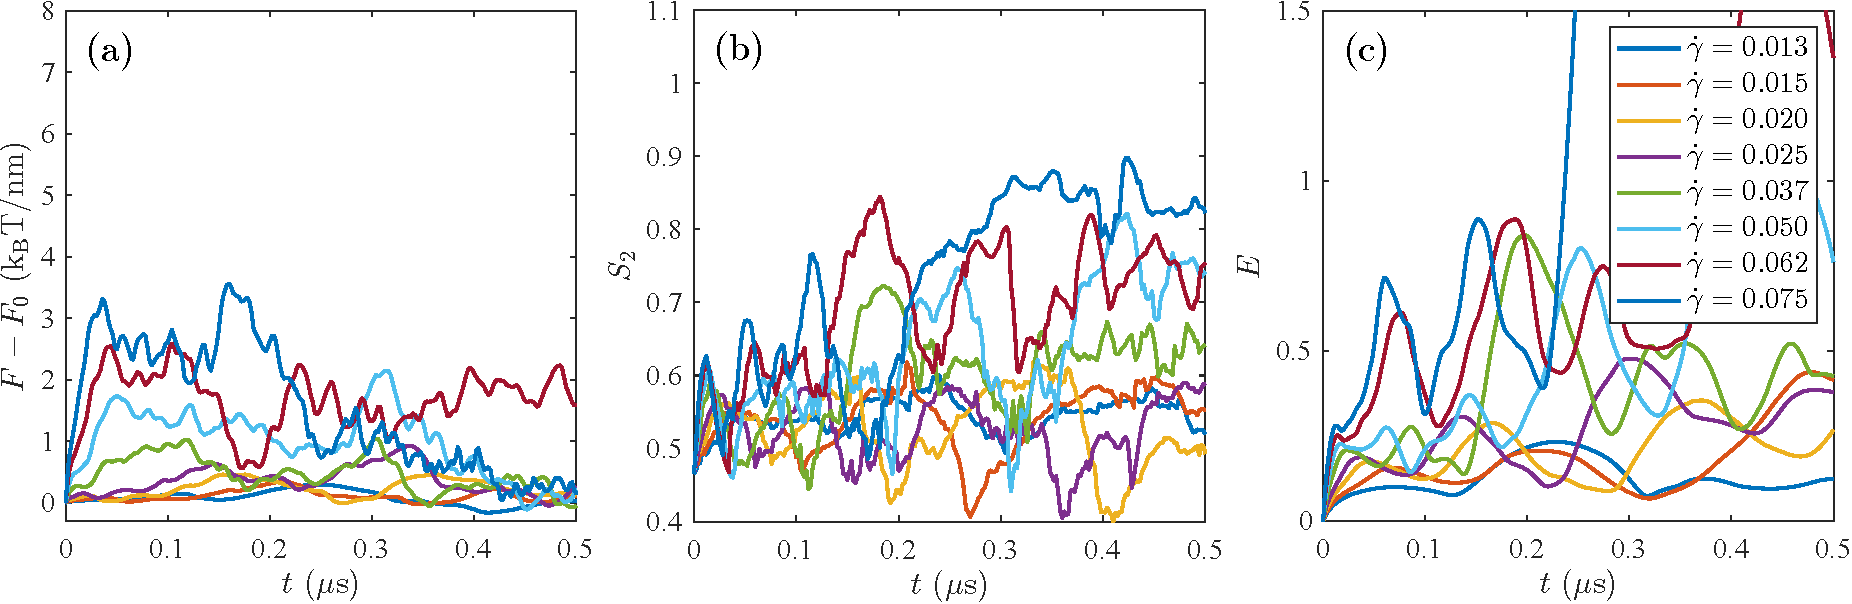
\includegraphics[width=\textwidth]{SMFigures/ULShRaw.pdf}
\end{center}
\caption{
Relative free energy $F - F_0$,
alignment $S_2$, and strain $E$ for
Type I, bilayer phase under shear flow with choices of shear rates $\dot\gamma=0.013$ -- $0.075$ ns$^{-1}$.
%The change in free energy $F$ is plotted in panel (a). Panel (b) shows the scalar order parameter $S_2$ over time $t$. Panel (c) plots the change of strain parameter $E$ in percentage over time $t$.
}
\label{fig:ulshraw}
\end{figure}


\begin{figure}[h!]
\begin{center}
\textbf{Type I, vesicle BL phase under shear flow}\par\medskip
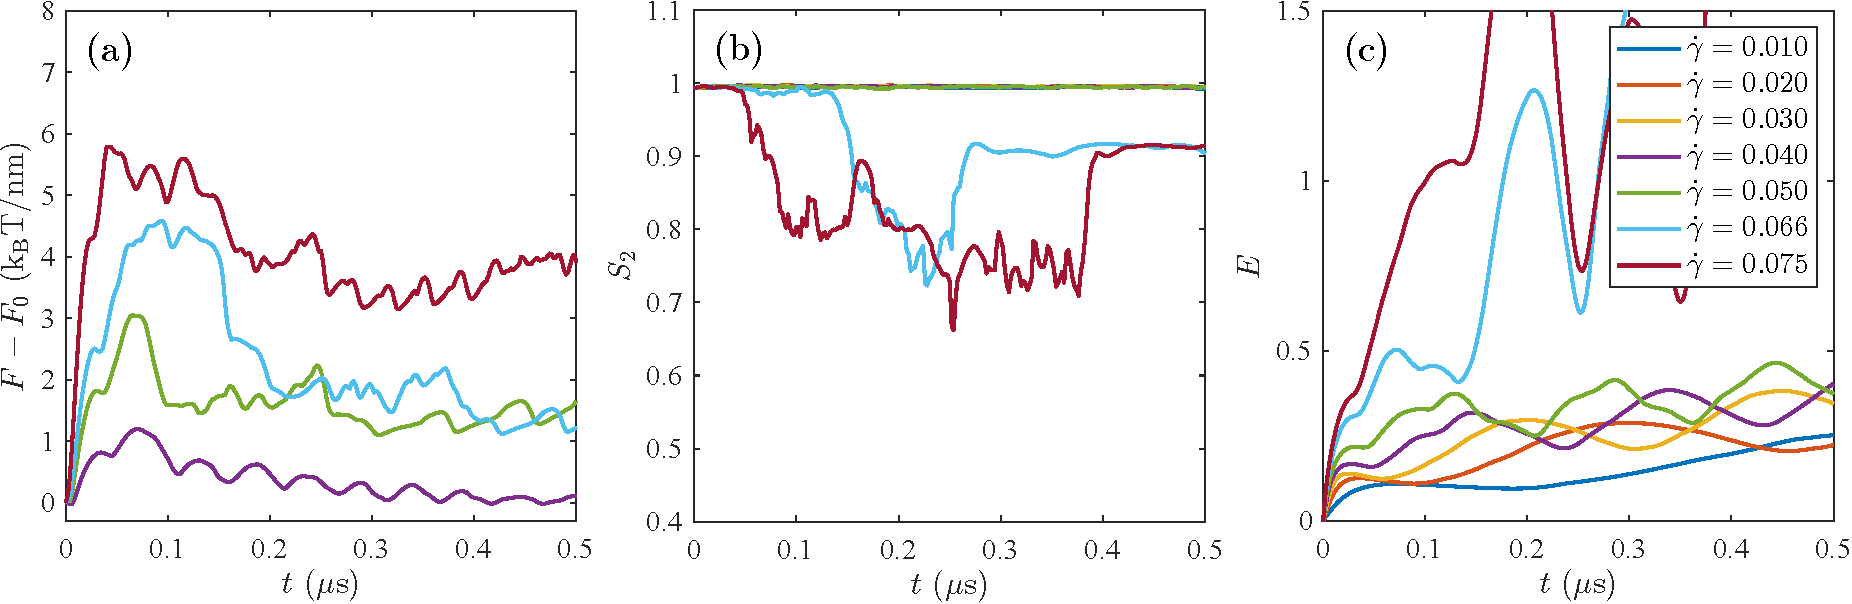
\includegraphics[width=\textwidth]{SMFigures/VeShRaw.pdf}
\end{center}
\caption{
Relative free energy $F - F_0$,
alignment $S_2$, and strain $E$ for
Type I, bilayer phase under shear flow with choices of shear rates $\dot\gamma=0.01$ -- $0.075$ ns$^{-1}$.
The JP type is the same as for Supplementary Figure \ref{fig:ulshraw} but with a
ring-shaped, rather than disordered, bilayer for initial configuration.  
%A Vesicle under a shear flow with choices of shear rates $\dot\gamma=0.01\sim0.075$. The change in free energy $F$ is plotted in panel (a). Panel (b) shows the scalar order parameter $S_2$ over time $t$. Panel (c) plots the change of strain parameter $E$ in percentage over time $t$.
}
\label{fig:veshraw}
\end{figure}


\begin{figure}[h!]
\textbf{Type II, multilamellar phase under shear flow}\par\medskip
\begin{center}
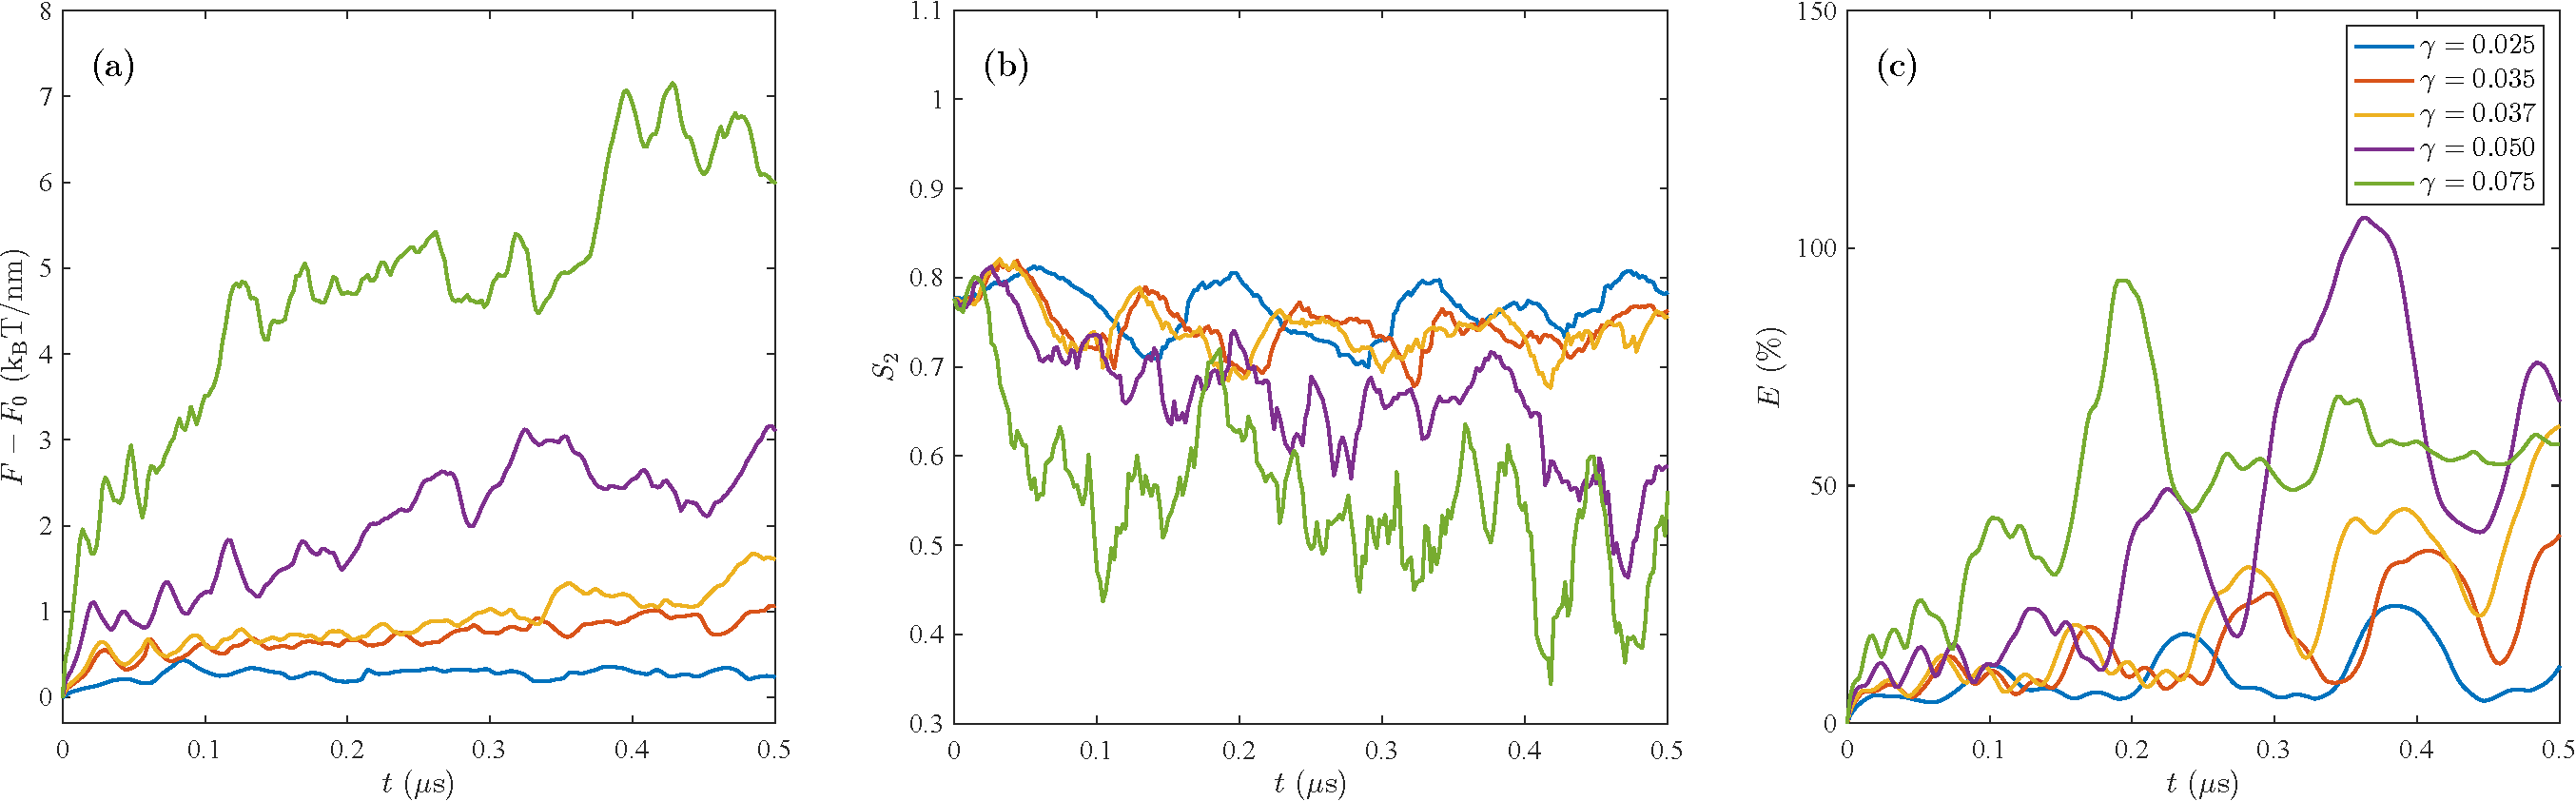
\includegraphics[width=\textwidth]{SMFigures/MLShRaw.pdf}
\end{center}
\caption{
Relative free energy $F - F_0$,
alignment $S_2$, and strain $E$ for
Type II, multilamellar phase under shear flow with choices of shear rates $\dot\gamma=0.025$ -- $0.075$ ns$^{-1}$.
%A multilamellar JP structure under a shear flow with choices of shear rates $\dot\gamma=0.025\sim0.075$. The change in free energy $F$ is plotted in panel (a). Panel (b) shows the scalar order parameter $S_2$ over time $t$. Panel (c) plots the change of strain parameter $E$ in percentage over time $t$.
}
\label{fig:mlshraw}
\end{figure}


\begin{figure}[h!]
\textbf{Type III, striated phase under shear flow}\par\medskip
\begin{center}
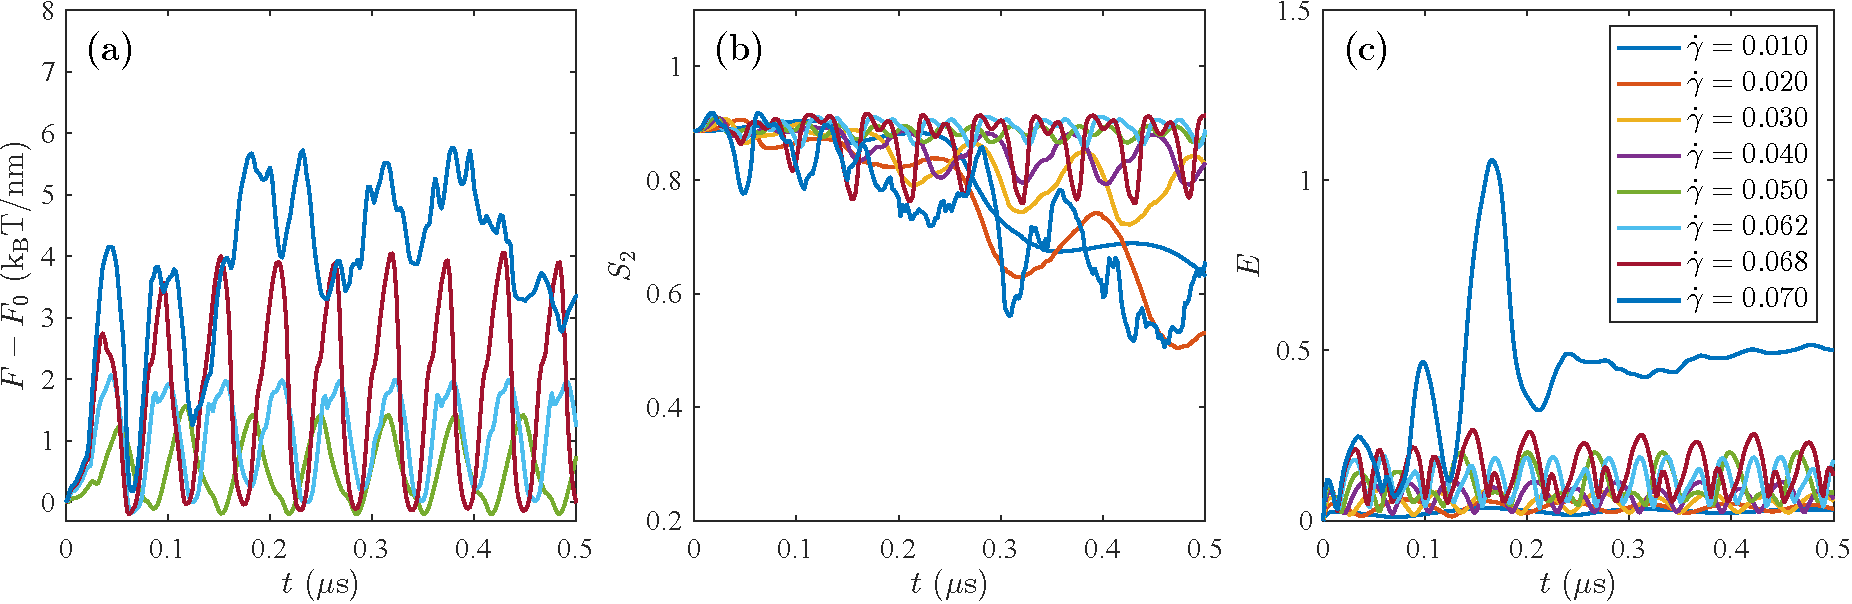
\includegraphics[width=\textwidth]{SMFigures/StShRaw.pdf}
\end{center}
\caption{
Relative free energy $F - F_0$,
alignment $S_2$, and strain $E$ for
Type III, striated phase under shear flow with choices of shear rates $\dot\gamma=0.01$ -- $0.07$ ns$^{-1}$.
%A striated JP structure under a shear flow with choices of shear rates $\dot\gamma=0.01\sim0.07$. The change in free energy $F$ is plotted in panel (a). Panel (b) shows the scalar order parameter $S_2$ over time $t$. Panel (c) plots the change of strain parameter $E$ in percentage over time $t$.
}
\label{fig:stshraw}
\end{figure}

\begin{figure}[h!]
\begin{center}
\textbf{\textsc{TG Flow Cases}}\par\medskip
\textbf{Type I, bilayer  phase under TG flow}\par\medskip
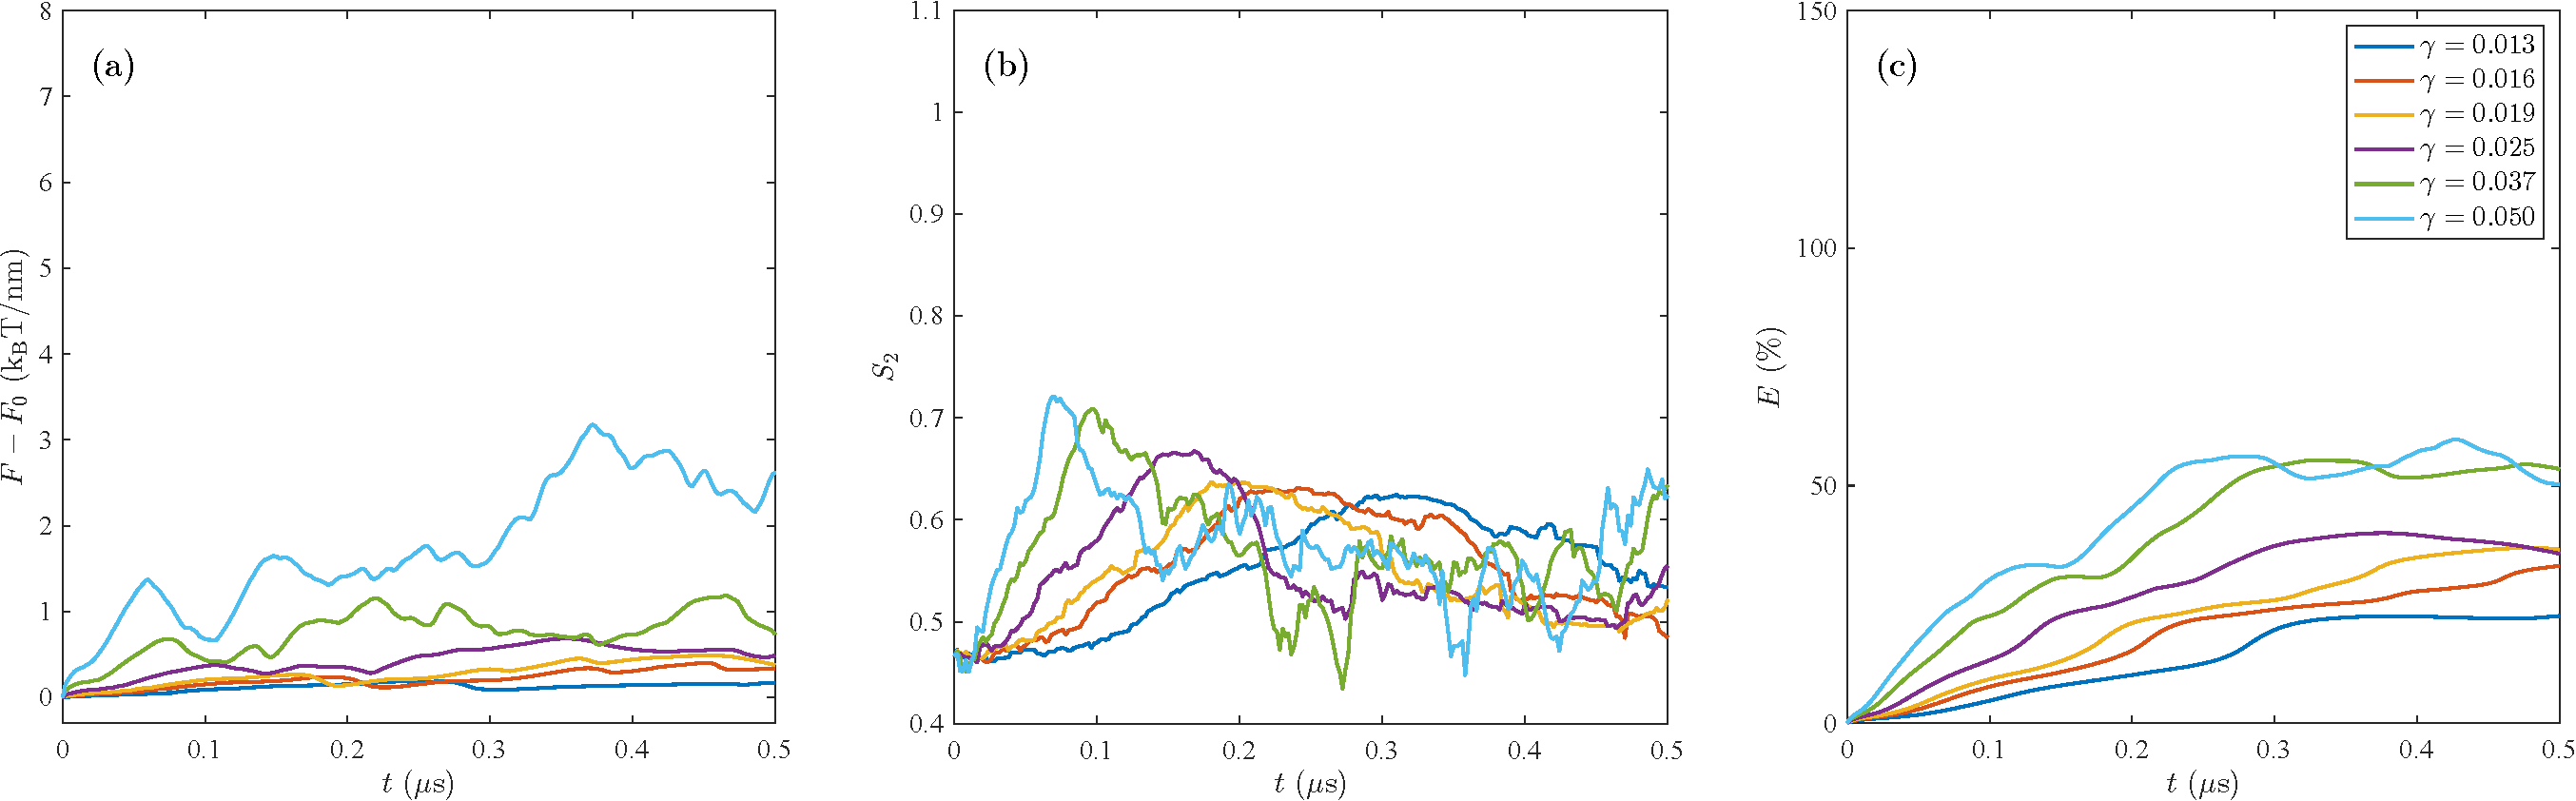
\includegraphics[width=\textwidth]{SMFigures/ULTGRaw.pdf}
\end{center}
\caption{
Relative free energy $F - F_0$,
alignment $S_2$, and strain $E$ for
Type I, bilayer phase under TG flow with choices of shear rates $\dot\gamma=0.013$ -- $0.05$ ns$^{-1}$.
%A unilamellar JP structure under a TG flow with choices of shear rates $\dot\gamma=0.013\sim0.05$. The change in free energy $F$ is plotted in panel (a). Panel (b) shows the scalar order parameter $S_2$ over time $t$. Panel (c) plots the change of strain parameter $E$ in percentage over time $t$.
}
\label{fig:ultgraw}
\end{figure}


\begin{figure}[h!]
\begin{center}
\textbf{Type I, vesicle BL phase under TG flow}\par\medskip
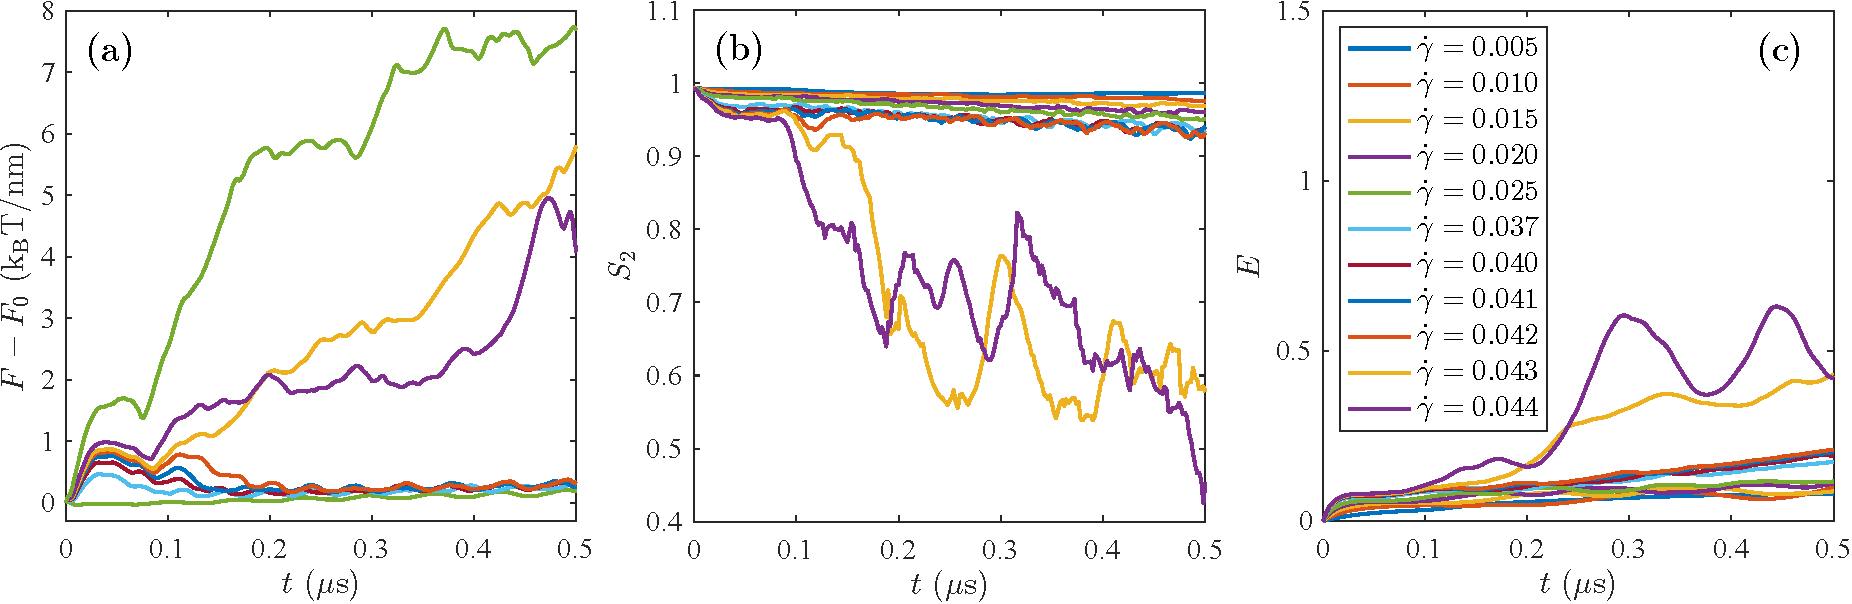
\includegraphics[width=\textwidth]{SMFigures/VeTGRaw.pdf}
\end{center}
\caption{
Relative free energy $F - F_0$,
alignment $S_2$, and strain $E$ for
Type I, vesicle bilayer phase under TG flow with choices of shear rates $\dot\gamma=0.005$ -- $0.044$ ns$^{-1}$.
The JP type is the same as for Supplementary Figure \ref{fig:ultgraw} but with a
ring-shaped, rather than disordered, bilayer for initial configuration.  
%A vesicle JP structure under a TG flow with choices of shear rates $\dot\gamma=0.005\sim0.044$. The change in free energy $F$ is plotted in panel (a). Panel (b) shows the scalar order parameter $S_2$ over time $t$. Panel (c) plots the change of strain parameter $E$ in percentage over time $t$.
}
\label{fig:vetgraw}
\end{figure}




\begin{figure}[h!]
\begin{center}
\textbf{Type II, multilamellar phase under TG flow}\par\medskip
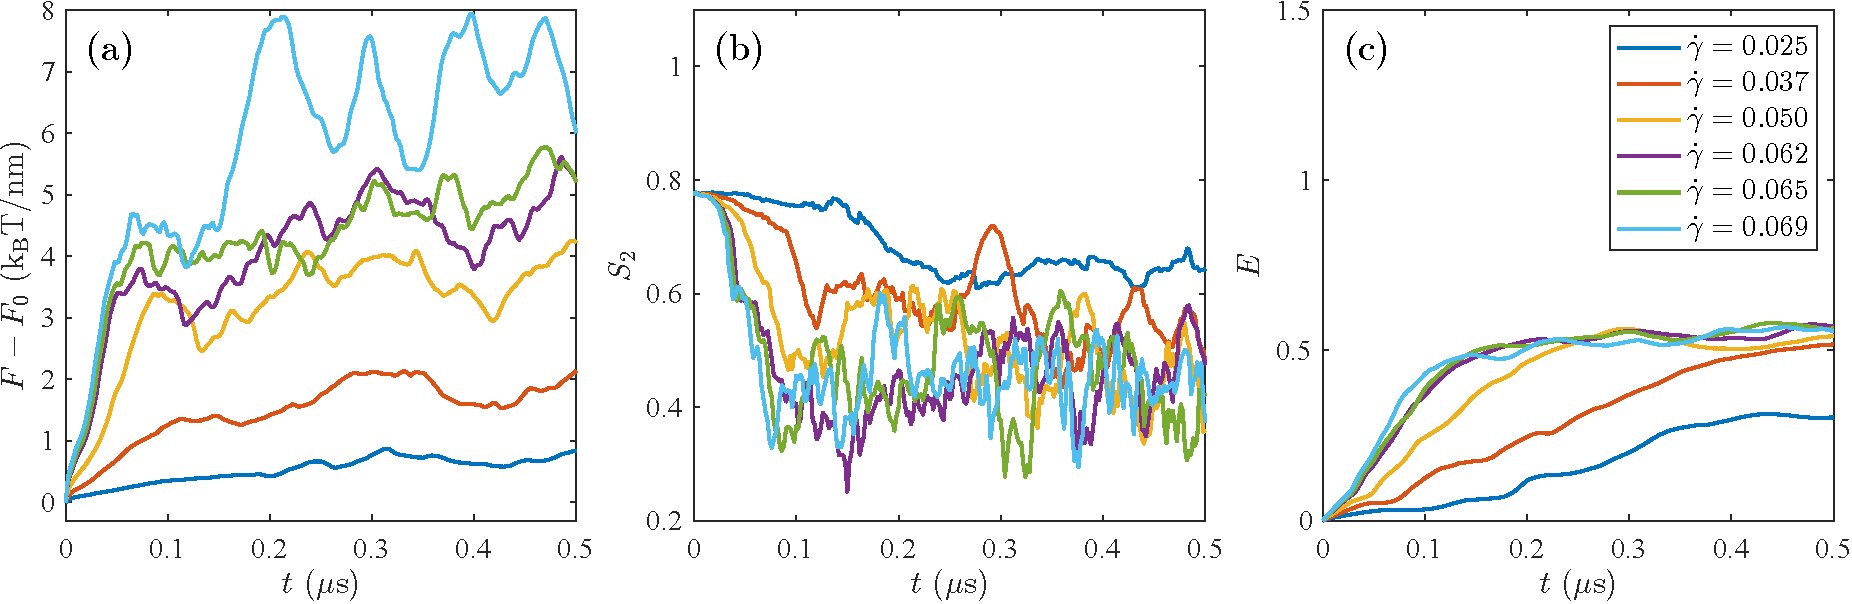
\includegraphics[width=\textwidth]{SMFigures/MLTGRaw.pdf}
\end{center}
\caption{
Relative free energy $F - F_0$,
alignment $S_2$, and strain $E$ for
Type II, multilamellar phase under TG flow with choices of shear rates $\dot\gamma=0.025$ -- $0.069$ ns$^{-1}$.
%A multilamellar JP structure under a TG flow with choices of shear rates $\dot\gamma=0.025\sim0.069$. The change in free energy $F$ is plotted in panel (a). Panel (b) shows the scalar order parameter $S_2$ over time $t$. Panel (c) plots the change of strain parameter $E$ in percentage over time $t$.
}
\label{fig:mltgraw}
\end{figure}


\begin{figure}[h!]
\begin{center}
\textbf{Type III, striated phase under TG flow}\par\medskip
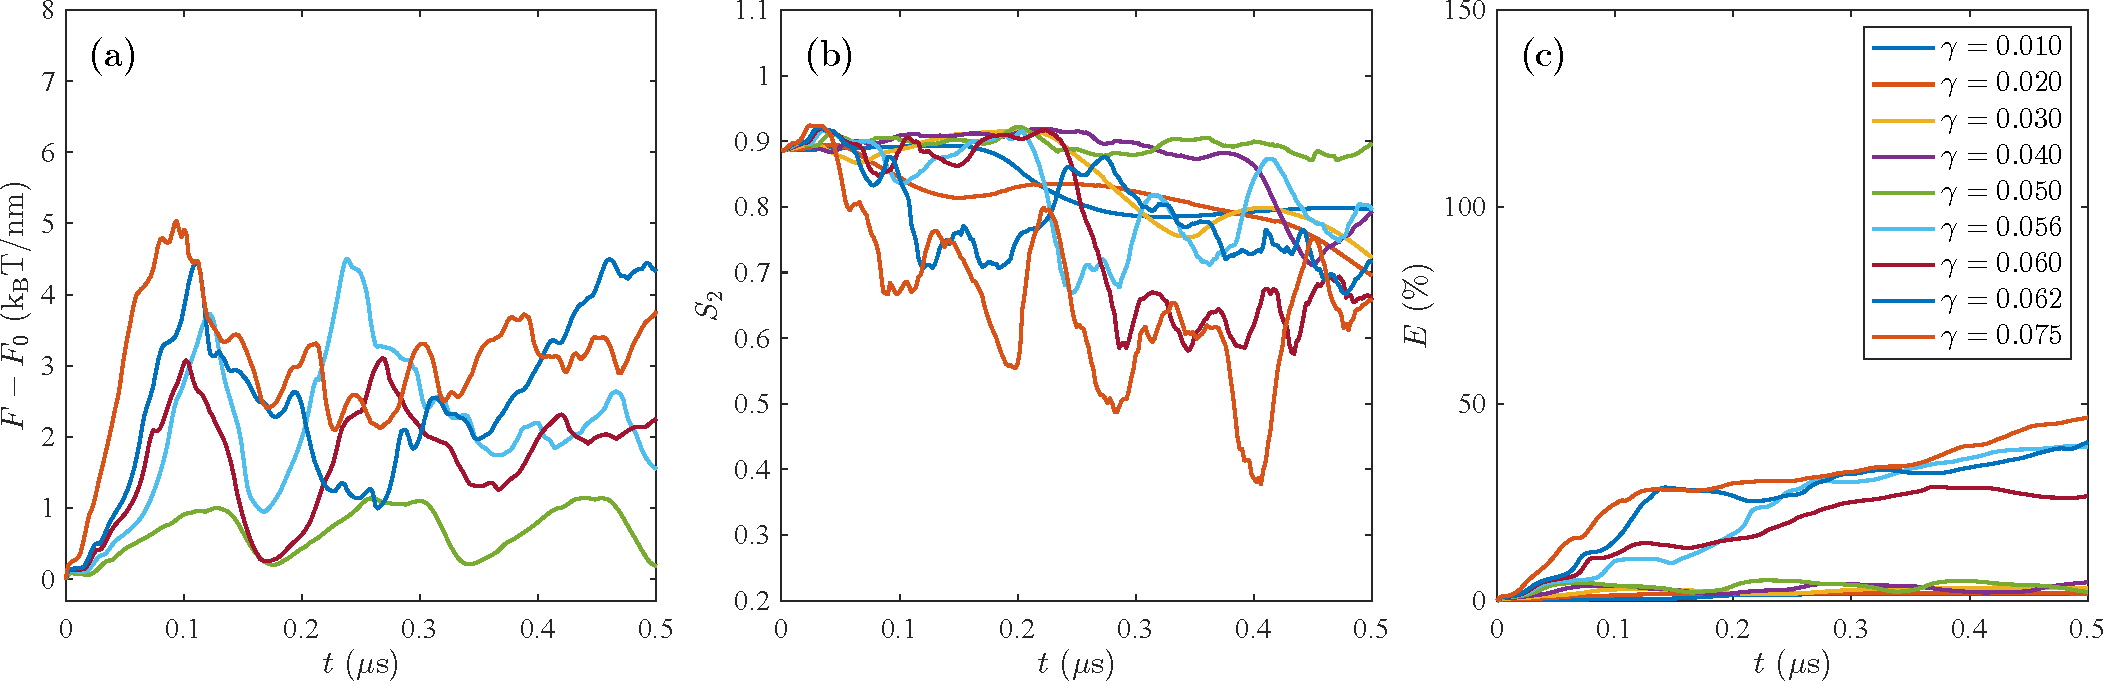
\includegraphics[width=\textwidth]{SMFigures/StTGRaw.pdf}
\end{center}
\caption{
Relative free energy $F - F_0$,
alignment $S_2$, and strain $E$ for
Type III, striated phase under TG flow with choices of shear rates $\dot\gamma=0.01$ -- $0.075$ ns$^{-1}$.
%A striated JP structure under a TG flow with choices of shear rates $\dot\gamma=0.01\sim0.069$. The change in free energy $F$ is plotted in panel (a). Panel (b) shows the scalar order parameter $S_2$ over time $t$. Panel (c) plots the change of strain parameter $E$ in percentage over time $t$.
}
\label{fig:sttgraw}
\end{figure}








\end{document}





%%%%%%%%%%%%%%%%%%%%%%%%%%%%%%%%%%%%%%%%%%%






\section{DRAFT RESULTS BELOW}
{\bf More results:}




\begin{figure}
  \begin{center}
  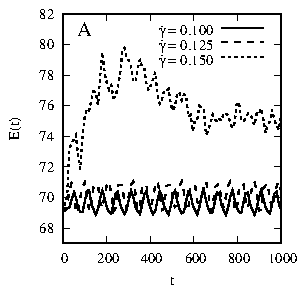
\includegraphics[width=0.3\textwidth]{CS_E.pdf}
   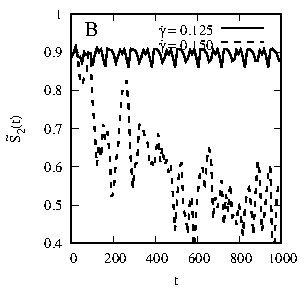
\includegraphics[width=0.3\textwidth]{CS_LOP.pdf}
    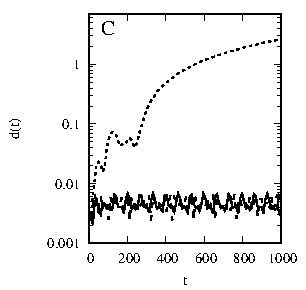
\includegraphics[width=0.3\textwidth]{CS_MSD.pdf}
  \end{center}
\caption{A checkerboard in shear flow with shear rates
  $\dot\gamma=\{0.125, 0.15\}$. We propose the order parameter defined
  by $S_{loc} = \frac12(3\cos(\theta-\bar\theta)^2-1)$}
\end{figure}


\begin{figure}
  \begin{center}
  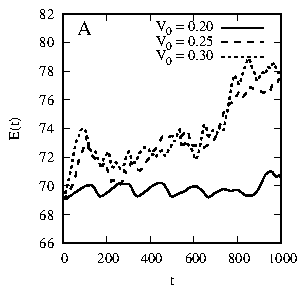
\includegraphics[width=0.3\textwidth]{CTG_E.pdf}
   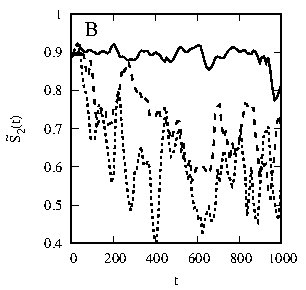
\includegraphics[width=0.3\textwidth]{CTG_LOP.pdf}
    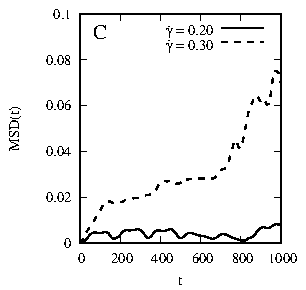
\includegraphics[width=0.3\textwidth]{CTG_MSD.pdf}
  \end{center}
\caption{A checkerboard in Taylor-Green flows when the flow strength $V_0=\{0.2,0.3\}$. }
\end{figure}






\subsubsection{}






%%%

\section{Governing Equations}
We consider a suspension of $N_b$ Janus particles in the fluid domain
$\Omega$.
The boundary of the $\Omega$ is $\bd\Omega = \Gamma_1 \cup
\cdots \cup \Gamma_{N_b}$, where $\Gamma_i$ is the boundary of Janus
particle $i$. We also consider a bounded fluid domain where $\Gamma_0$
is the fixed boundary of $\Omega$. In this case, $\bd\Omega = \Gamma_0
\cup \Gamma_1 \cup \cdots \cup \Gamma_{N_b}$.

%%%
\subsection{Hydrophobic Attraction Potential Mobility Problem} 
The mathematical formulation is a nonlinear system for the dynamics of a
collection of rigid Janus particles. For the sake of completeness, we
summarize the governing equations here, and a complete description is in
our previous work~\cite{Fu2022_JFM}. The interactions satisfy a
system of partial differential equations (PDEs) that describe the
hydrodynamic interactions and hydrophobic interactions. Assuming
inertial terms are negligible, the solvent is governed by the Stokes
equations
\begin{alignat}{3}
\label{eq:stokes}
  -\mu \Delta \uu + \nabla p &= \mathbf{0},     && \xx \in \Omega, \\
  \nabla\cdot \uu &= 0, \qquad && \xx \in \Omega, \\
  \uu - \uu_\infty &\to \mathbf{0}, && |\xx| \to \infty,
\end{alignat}
where $\uu$ is the velocity, $p$ is the pressure, $\uu_\infty$ is the
background flow, and $\mu$ is the (constant) solvent viscosity. The domain $\Omega
= \Omega(t)$ is the fluid region surrounding the particles and changes
shape as the particles move. Since the particles are rigid, the solvent
velocity satisfies the no-slip rigid body motion boundary condition
\begin{align}
  \vv_i + \omega_i (\xx - \aa_i)^\perp = \uu(\xx), 
    \quad \xx \in \Gamma_i,
\end{align}
where $\vv_i$ is the translational velocity and $\omega_i$ is the
angular velocity. Once these velocities are determined, we use
second-order Adams-Bashforth to update the particle configuration. 

The translational and angular velocities guarantee that the fluid forces
balance the imposed forces. The imposed forces include the hydrophobic
interactions that arise so that particles minimize the free energy of
the structure of the surrounding water molecules. The free energy
functional is
\begin{align}
\label{eq:free_energy}
  F[u] = C \int_{\Omega} \left(\rho |\nabla u|^2 + \rho^{-1} f(u)\right)
  \,d\xx,
\end{align}
where $u$ is an order parameter for the structure of water, $\rho$ is a
decay length, $C$ is a constant, and $f(u)$ is a potential.
%$c$ is ``effective" inter-particle distance below which the steric repulsion becomes important.
Hydrogen-bond persistence times are on the order of picoseconds which is
much smaller than characteristic time for particle motion.
%\cite{MaGa13}. 
Thus we assume $u$ minimizes $F[u]$ for all times. Assuming appropriate
conditions on $f(u)$,
% (\cite{evans10}, \S 8.2),
$u$ satisfies the Euler-Lagrange equation
\begin{alignat}{3}
  \label{eq:SL}
  -\rho^2 \Delta u + \tfrac{1}{2}f'(u) &= 0, && \xx \in \Omega, \\
  u &= g, && \xx \in \bd\Omega, \\
  u &\rightarrow 0, \qquad&& |\xx| \rightarrow \infty.
\end{alignat}
Equation~\eqref{eq:SL} is solved with a boundary integral equation
method. The boundary condition $g$ is a material label that is
transported with the particle.

The particles lower the free energy $F[u]$ of the surrounding water
by moving. We calculate the rate of change of $F[u]$ using
variation of the domain. % ~\cite{Fu2018_SIAM,Bandle2015, Schiffer1954, Grinfeld2010}.
Carrying out this variation yields the stress  
\begin{align}
  \label{eq:stress}
\mathbf{T}
= C \left[ \rho^{-1} f(u) \mathbf{I}
  + \rho \left(|\nabla u|^2 \mathbf{I} - 
  2\nabla u \nabla u^T\right)\right].
\end{align}
The imposed forces and torques come from the integration of $\mathbf{T}$
along the particle boundary. These forces and torques couple the Stokes
equations \eqref{eq:stokes}, to semilinear elliptic equation
\eqref{eq:SL}. Solving for the translational and rotational velocities
gives the particle evolution.

To solve the Stokes equation with the correct boundary conditions, we
represent the velocity as the of a layer potential with Stokeslets and
rotlets
\begin{align}
  \label{eq:velocity}
  \uu(\xx) = \uu_\infty(\xx) + \DD[\eeta](\xx) + 
    \sum_{i=1}^{N_b} \left(\SS(\xx,\aa_i) \cdot \FF_i + 
    \RR(\xx,\aa_i) T_i\right), \quad \xx \in \Omega.
\end{align}
%
Then, the density function $\eeta$, translation velocity $\vv_i$ and
angular velocity $\omega_i$ satisfy
\begin{alignat}{3}
  \nonumber
  \vv_i + \omega_i (\xx - \aa_i)^\perp &= \uu_\infty(\xx)
    -\frac{1}{2} \eeta(\xx) + \DD[\eeta](\xx) \\
  \label{eq:SKIE}
    + \sum_{j=1}^{N_b} &
    \left(\SS(\xx,\aa_j) \cdot \FF_j + \RR(\xx,\aa_j) T_j\right),
    \quad &&\xx \in \Gamma_i,\: i=1,\ldots,N_b, \\
  \label{eq:mobility1}
  \int_{\Gamma_i} \eeta \, \dif s &= \mathbf{F}_i, 
  &&i = 1,\ldots,N_b, \\
  \label{eq:mobility2}
  \int_{\Gamma_i} \eeta \cdot (\xx-\aa_i)^\perp \, \dif s &= T_i,
  &&i = 1,\ldots,N_b.
\end{alignat}

\subsection{Normal Derivative of Double Layer Potential and HAP Energy}

We adopt the double layer potential to express the solution of \eqref{eq:SL} where the
condition is $f(u)=u^2$. Then it is given by 
\begin{align}
\label{eq:energy_BIE}
u({\bf x}) = \DD[\sigma](\xx) = \int_\Gamma \frac{\partial G(\xx-\yy)}{\partial \nnu_\yy}\sigma(\yy)\, \dif s_\yy,
\end{align}
%
where $G(\xx)$ is the fundamental solution to the screened Laplace
equation \eqref{eq:SL} and $\nnu_\yy$ is the outward normal.
Since the free energy functional can be written as 
\begin{align}
\label{eq:free_energy2}
  E[u(\xx)] &= C\rho \int_\Gamma u \frac{\partial u}{\partial \nnu}  \,\dif s, \quad \xx\in\Gamma_i,
\end{align}
%
we can then refer to the identity (\cite{Hsiao2008}, \S 1.2) to calculate this boundary integral equation without evaluating the normal derivative of the double layer potential directly.

Consider
\begin{align}
\nnu_\xx \cdot \nabla_\zz u(\zz) &=\nnu_\xx \cdot \nabla_\zz \int_\Gamma \frac{\partial G(\zz-\yy)}{\partial \nnu_\yy}\sigma(\yy) \,\dif s_\yy\\
&=\int_\Gamma \nnu_\xx\cdot \left(\nabla_\zz\nabla_\yy^\top  G(\zz-\yy)\right)\cdot \nnu_\yy\sigma(\yy)  \,\dif s_\yy\\
&=-\int_\Gamma \nnu_\xx\cdot \left(\nabla_\yy\nabla_\yy^\top G(\zz-\yy)\right)\cdot\nnu_\yy\sigma(\yy)\ \dif s_\yy\\
&=-\int_\Gamma {\bf t}_\xx\cdot\Delta_\yy G(\zz-\yy) {\bf t}_\yy \sigma(\yy)\ \dif s_\yy+\int_\Gamma({\bf t}_\xx\cdot\nabla_\yy)({\bf t}_\yy\cdot\nabla_\yy G(\zz-\yy))\sigma(\yy)\ \dif s_\yy\\
&= -\int_\Gamma {\bf t}_\xx\cdot\frac1\rho^2 G(\zz-\yy) {\bf t}_\yy \sigma(\yy)\ \dif s_\yy - 
({\bf t}_\xx\cdot\nabla_\zz)\int_\Gamma \frac{\partial G(\zz-\yy)}{\partial s_\yy}\sigma(\yy)\ \dif s_\yy\\
&= -\frac1\rho^2 {\bf t}_\xx\cdot \int_\Gamma G(\zz-\yy){\bf t}_\yy \sigma(\yy)\ \dif s_\yy + 
({\bf t}_\xx \cdot \nabla_\zz)\int_\Gamma G(\zz-\yy)\frac{\partial \sigma(\yy)}{\partial s}\ \dif s_\yy.
\end{align}
%
Here ${\bf t}_\xx$ is the tangent vector at the point $\xx$ and $d/ds$ is the arclength derivative.
Letting $\zz\to\xx\in\Gamma$, we obtain
%
\begin{equation}
\label{eq:normal_deriv}
\frac{\partial}{\partial \nnu_\xx} \DD[\sigma](\xx) = -\frac1\rho^2 {\bf t}_\xx\cdot \SSS[\sigma{\bf t}](\xx) + \frac{\partial}{\partial s}\SSS\left[\frac{\partial \sigma}{\partial s}\right](\xx).
\end{equation}
%

Substituting \eqref{eq:normal_deriv} to \eqref{eq:free_energy2} provides the total energy calculation
throughout this paper and this expression takes the advantage of not calculating the quadruple layer potential which has well-known obstacle in numerical implementation.

%Suppose we split the solution to the screened Laplace boundary value problem~\eqref{eq:SL}
%into smooth portion $w_i$ and singular portion $u_i$. That is, 
%\begin{equation}
%w_i({\bf x}) = u({\bf x}) - u_i = u({\bf x}) - \int_{\Gamma_i }\left(\pderiv{}{\nnu_\yy}
%    K_0 \left(\frac{|\xx - \yy|}{\rho}\right)\right) \sigma_i(\yy) \,
%    \dif s_\yy, \quad \xx \in \Gamma_i.
%\end{equation}
%Consider the case when $f(u)=u^2$ in~\eqref{eq:free_energy}, we can rewrite the free energy functional as 
%
%\begin{align}
%\label{eq:free_energy2}
%  E[u(\xx)] &= C\rho \sum_{i=1}^{N_b}\int_{\Gamma_i} u \frac{\partial u}{\partial \nnu}  \,\dif s
%= C\rho\sum_{i=1}^{N_b}\int_{\Gamma_i} u \left(\frac{\partial w_i}{\partial \nnu}+\frac{\partial u_i}{\partial \nnu} \right) \, \dif s, \quad \xx\in\Gamma_i.
%\end{align}
%%%%
%Follow the divergence theorem on the last term in the equation above and denote $g_i(x)$ as the boundary data on $\Gamma_i$, we obtain
%\begin{align}
%\label{eq:free_energy3}
%  E[u(\xx)] &= C\rho\sum_{i=1}^{N_b}\left(\int_{\Gamma_i} u \frac{\partial w_i}{\partial \nnu} \,\dif s  + \int_{\mathbb{R}^n\setminus \overline{U}_i} \left( \nabla u \cdot\nabla u_i + u\Delta u_i\right) \,\dif \xx\right)\\
%%
%&= C\rho\sum_{i=1}^{N_b}\left(\int_{\Gamma_i} u \frac{\partial w_i}{\partial \nnu} \,\dif s  + \int_{\mathbb{R}^n\setminus \overline{U}_i} u\Delta u_i\,\dif \xx
%+\int_{\Gamma_i}\left(u+\frac12\sigma\right)\frac{\partial u_i}{\partial \nnu} \,\dif s     
%- \int_{\mathbb{R}^n\setminus \overline{U}_i} u\Delta u_i\,\dif \xx \right)\\
%&= C\rho\sum_{i=1}^{N_b}\left(\int_{\Gamma_i} u \frac{\partial w_i}{\partial \nnu} + 
%\left(g_i+\frac12\sigma_i\right)\frac{\partial u_i}{\partial \nnu}   \,\dif s \right), \quad \xx \in \Gamma_i.
%\end{align}
%
%
%

%  &= C\rho\sum_{i=1}^{N_b}\left(\int_{\Gamma_i} g_i \frac{\partial w_i}{\partial \nnu} 
% +  \left(u_i+\frac12\sigma\right)  \frac{\partial g_i}{\partial \nnu} \,\dif s - \int_{\mathbb{R}^n\setminus \overline{U}_i}\Delta g_i  \left(u_i+\frac12\sigma\right)  - g_i \left(u_i+\frac12\sigma\right) \,\dif \xx\right) \\
% &= C\rho\sum_{i=1}^{N_b}\int_{\Gamma_i} g_i \frac{\partial w_i}{\partial \nnu}+ \left(u_i+\frac12\sigma\right)  \frac{\partial g_i}{\partial \nnu}\,\dif s, \quad \xx\in\Gamma_i.



%%
%$\sigma$ satisfies the second-kind integral equation
%\begin{equation}
%\label{eq:screenedSKIE}
%  g(\xx) = \frac{1}{2}\sigma(\xx) + 
%    \frac{1}{2\pi}\int_{\bd\Omega} \left(\pderiv{}{\nnu_\yy}
%    K_0 \left(\frac{|\xx - \yy|}{\rho}\right)\right) \sigma(\yy) \, 
%    \dif s_\yy, \quad \xx \in \bd\Omega,
%\end{equation}

\section{Numerical Results}

\subsection{Self-Assembled Janus Particle with Specific Boundary Conditions}

Distinct morphologies can be obtained from 
the HAP model by shifting the boundary condition $g(\xx)$.
Consider the linear case where $f(u) = u^2$.
This choice makes \eqref{eq:SL} a boundary value
problem for the screened-Laplace equation
and the solutions have a boundary layer structure that decays to $0$ in the
bulk with the decay length $\rho$.
We consider three kinds of boundary conditions
on particle $\Gamma_i$:
\begin{equation}
  \label{eq:bcs}
  \begin{tabular}{c|c|c}
     \text{(i)} & \text{(ii)} & \text{(iii)} \\
    \hline
    \rule{0pt}{4ex} 
      $g(\mathbf{x}) = \displaystyle \frac{1+\cos (\theta_i(\xx))}{\sqrt{3\pi r}}$
    & $g(\mathbf{x}) = \displaystyle \frac{2+\cos (\theta_i(\xx))}{\sqrt{9\pi r}}$
    & $g(\mathbf{x}) = \displaystyle \frac{\cos (\theta_i(\xx))}{\sqrt{\pi r}}$
\end{tabular}
\end{equation}
The number $\theta_i(\xx)$ is the angle formed by the position $\xx$,
the particle center $\aa_i$, and the particle director $\dd_i$.
(Figure~\ref{fig:flow_map}). The normalizations e.g., $(\pi r)^{-1/2}$,
provide a uniform surface energy $\int_{\Gamma_i} g^2 \,ds = 1$ for
circular particles of radius $r$. The cases (ii) and (iii) are obtained
by applying a vertical shift and scaling to case (i). Using this setup,
we simulate the dynamics of 60 particles with one set of random initial
positions and orientations as shown in Figure~\ref{fig:relax}(a)

\begin{figure}
  \begin{center}
  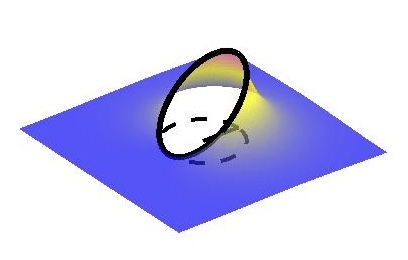
\includegraphics[width=0.2\textwidth]{LPA.jpg}
  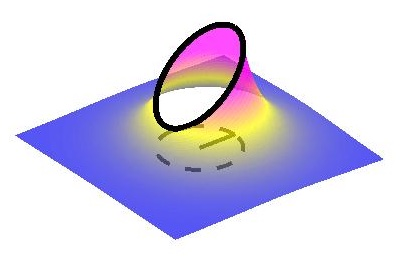
\includegraphics[width=0.2\textwidth]{LPB.jpg}
  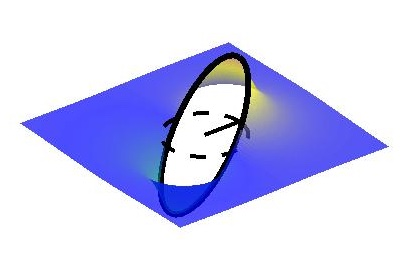
\includegraphics[width=0.2\textwidth]{LPC.jpg}
  \end{center}
  \vspace{-20pt}  
  \caption{\label{fig:bcs} Boundary conditions characterize the water
  structure at the particle interface: an amphiphilic particle (left), a
  hydrophobic particle with anisotropic intensity (middle), a water
  structure with positive/negative charge (right). The dashed curve is
  the boundary of the disk and the arrow is its director for each
  particle.}
\end{figure}


\begin{figure}
  \begin{center}
  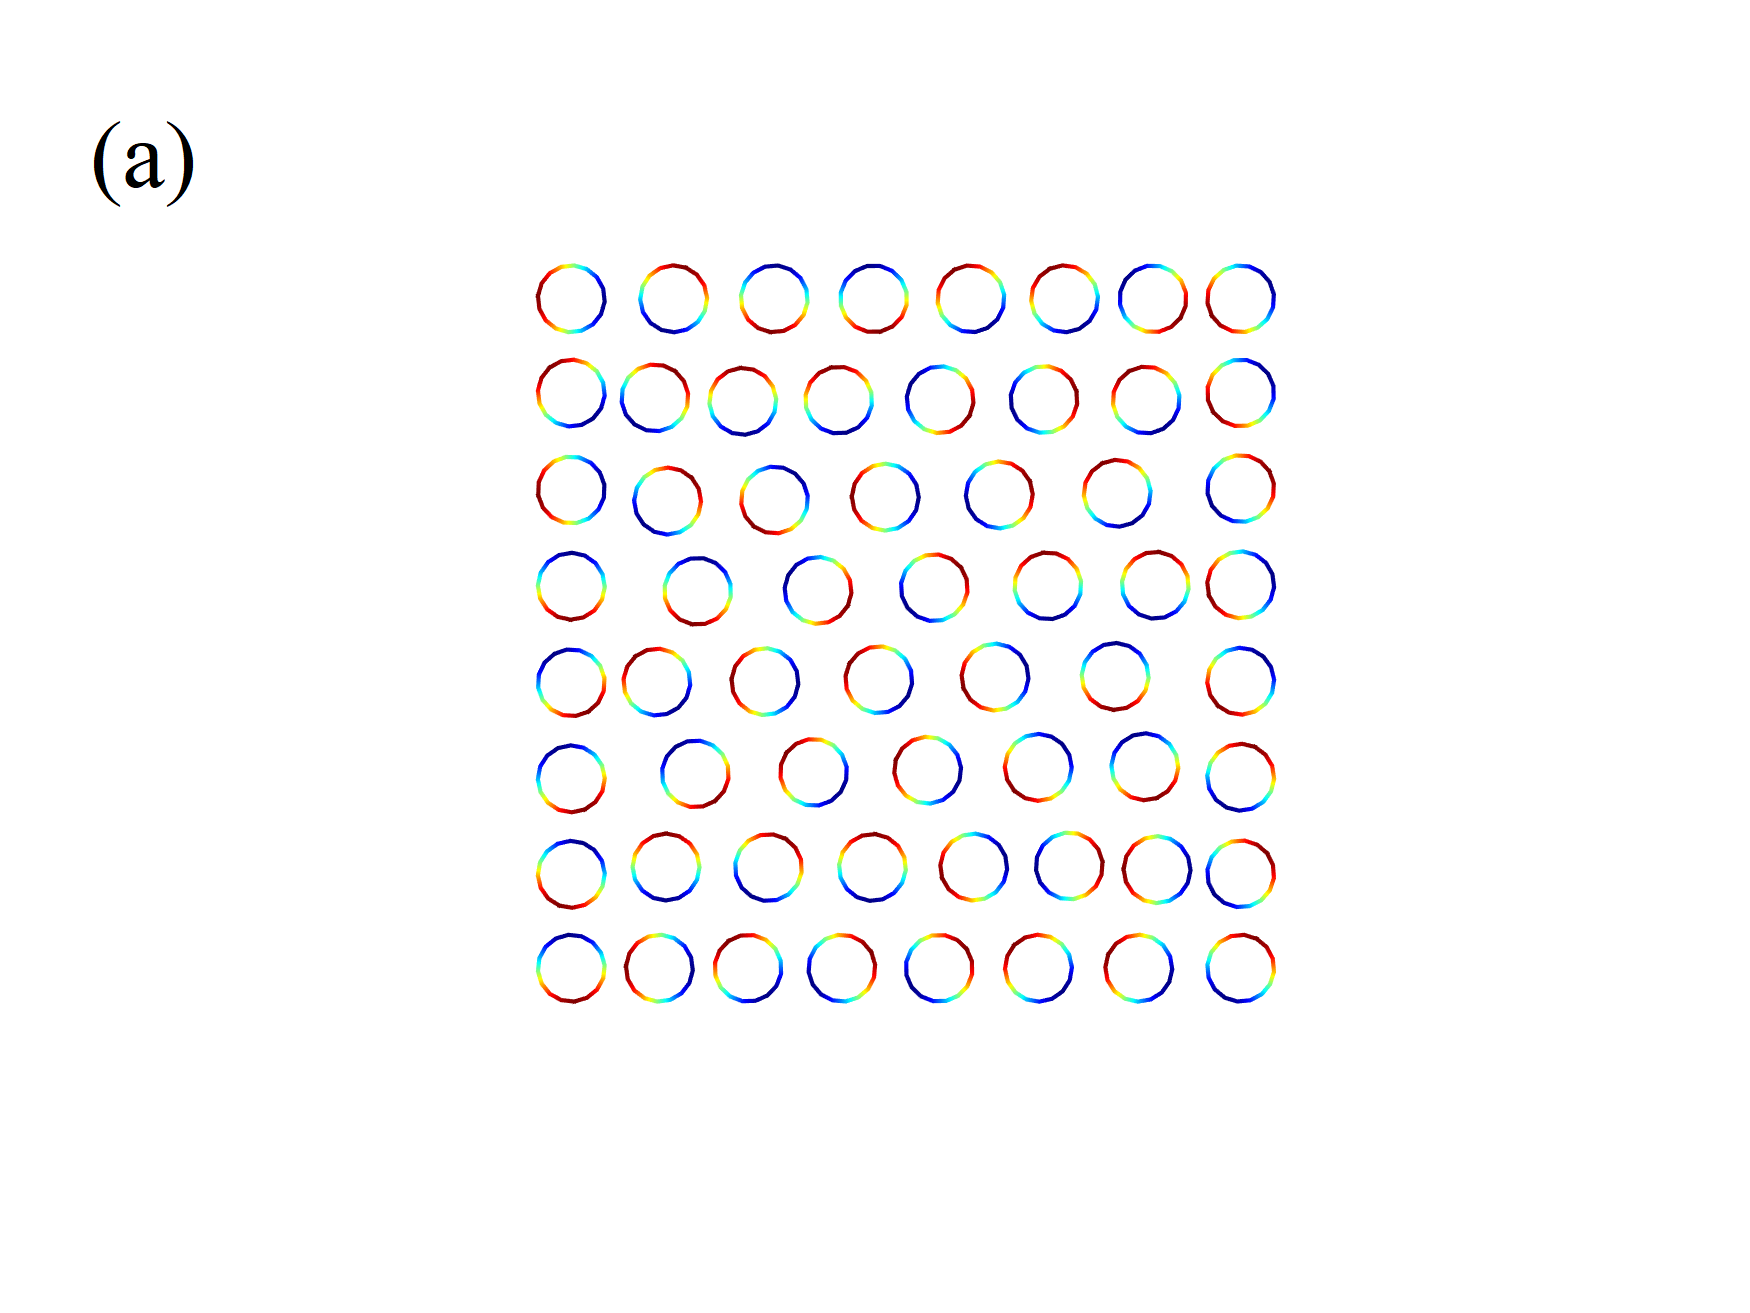
\includegraphics[width=0.4\textwidth]{Fig2a.png}
  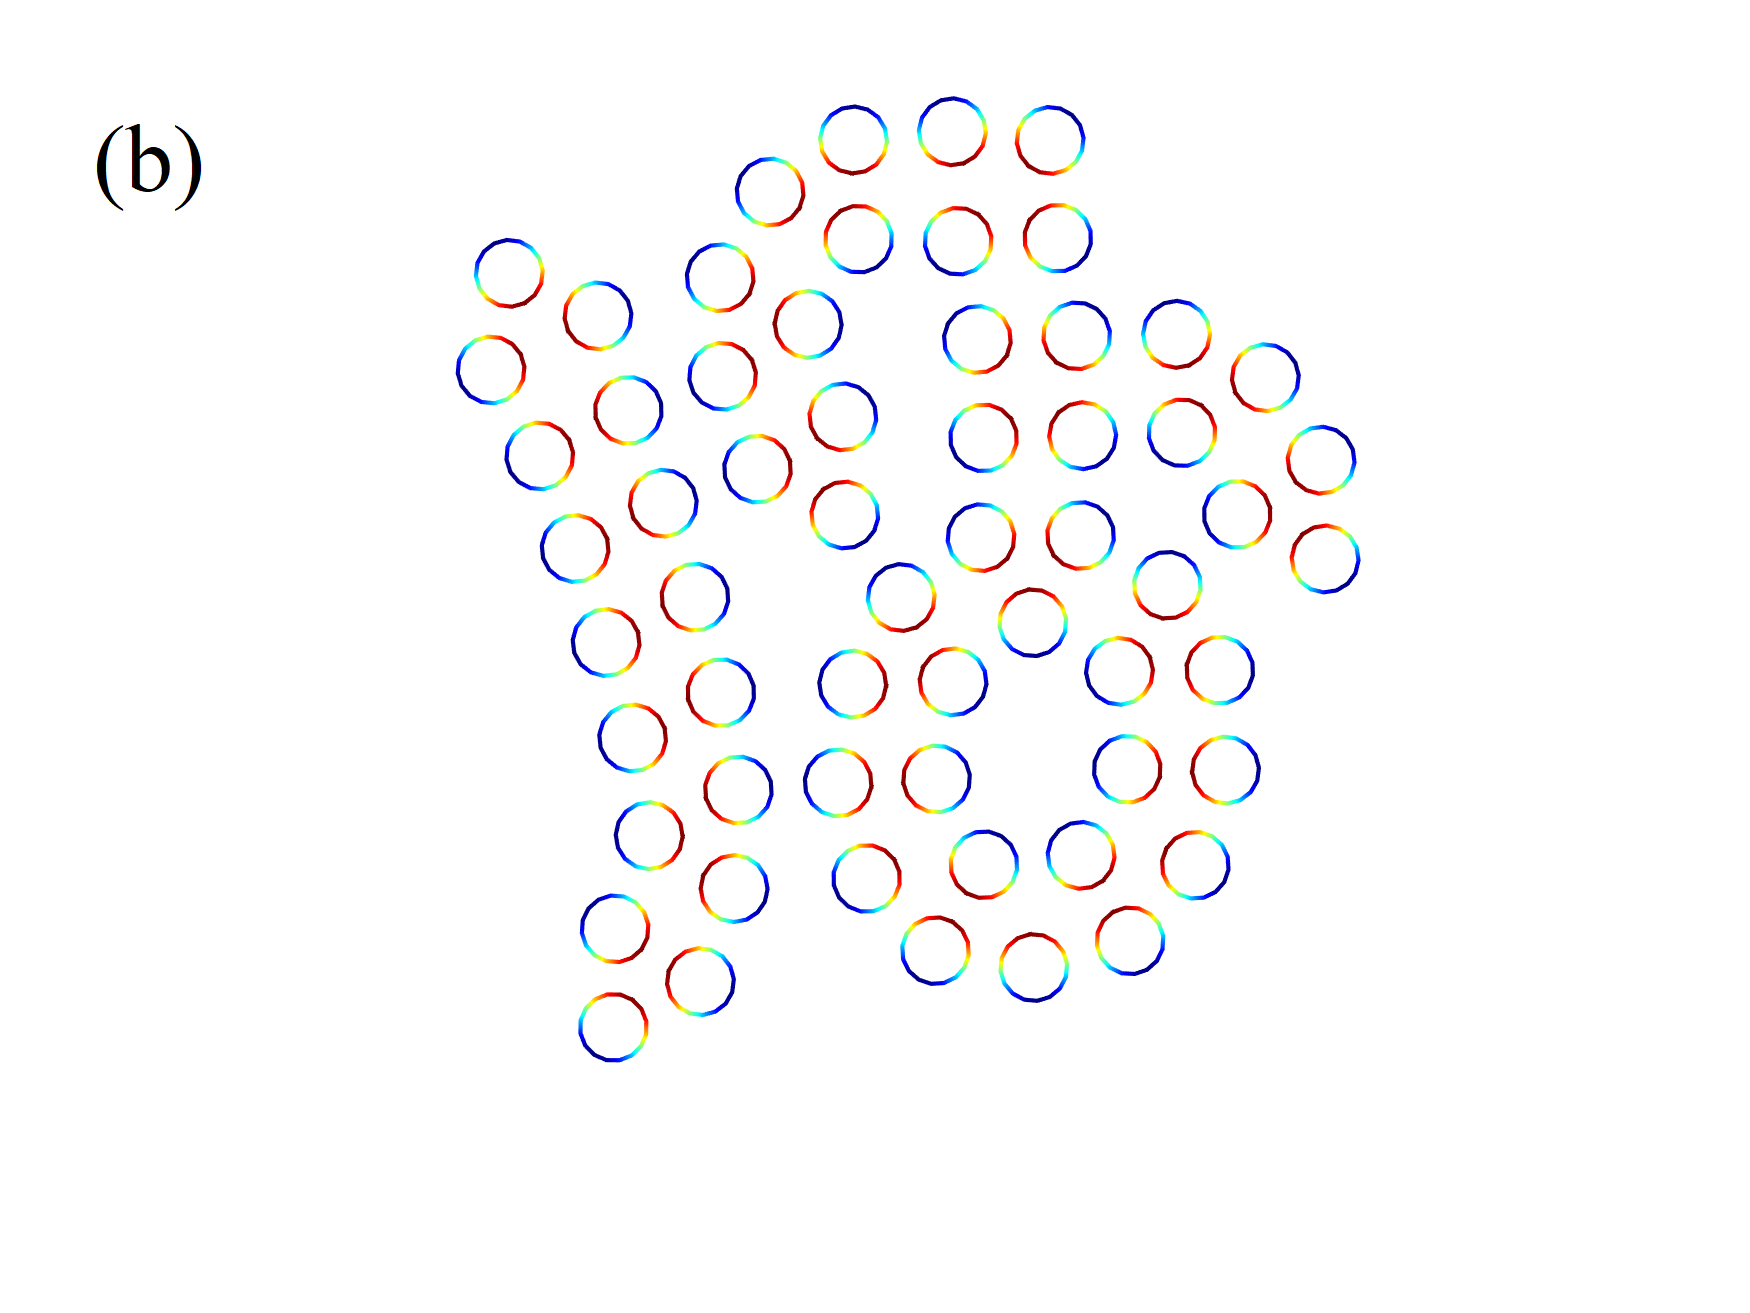
\includegraphics[width=0.4\textwidth]{Fig2b.png}\\
  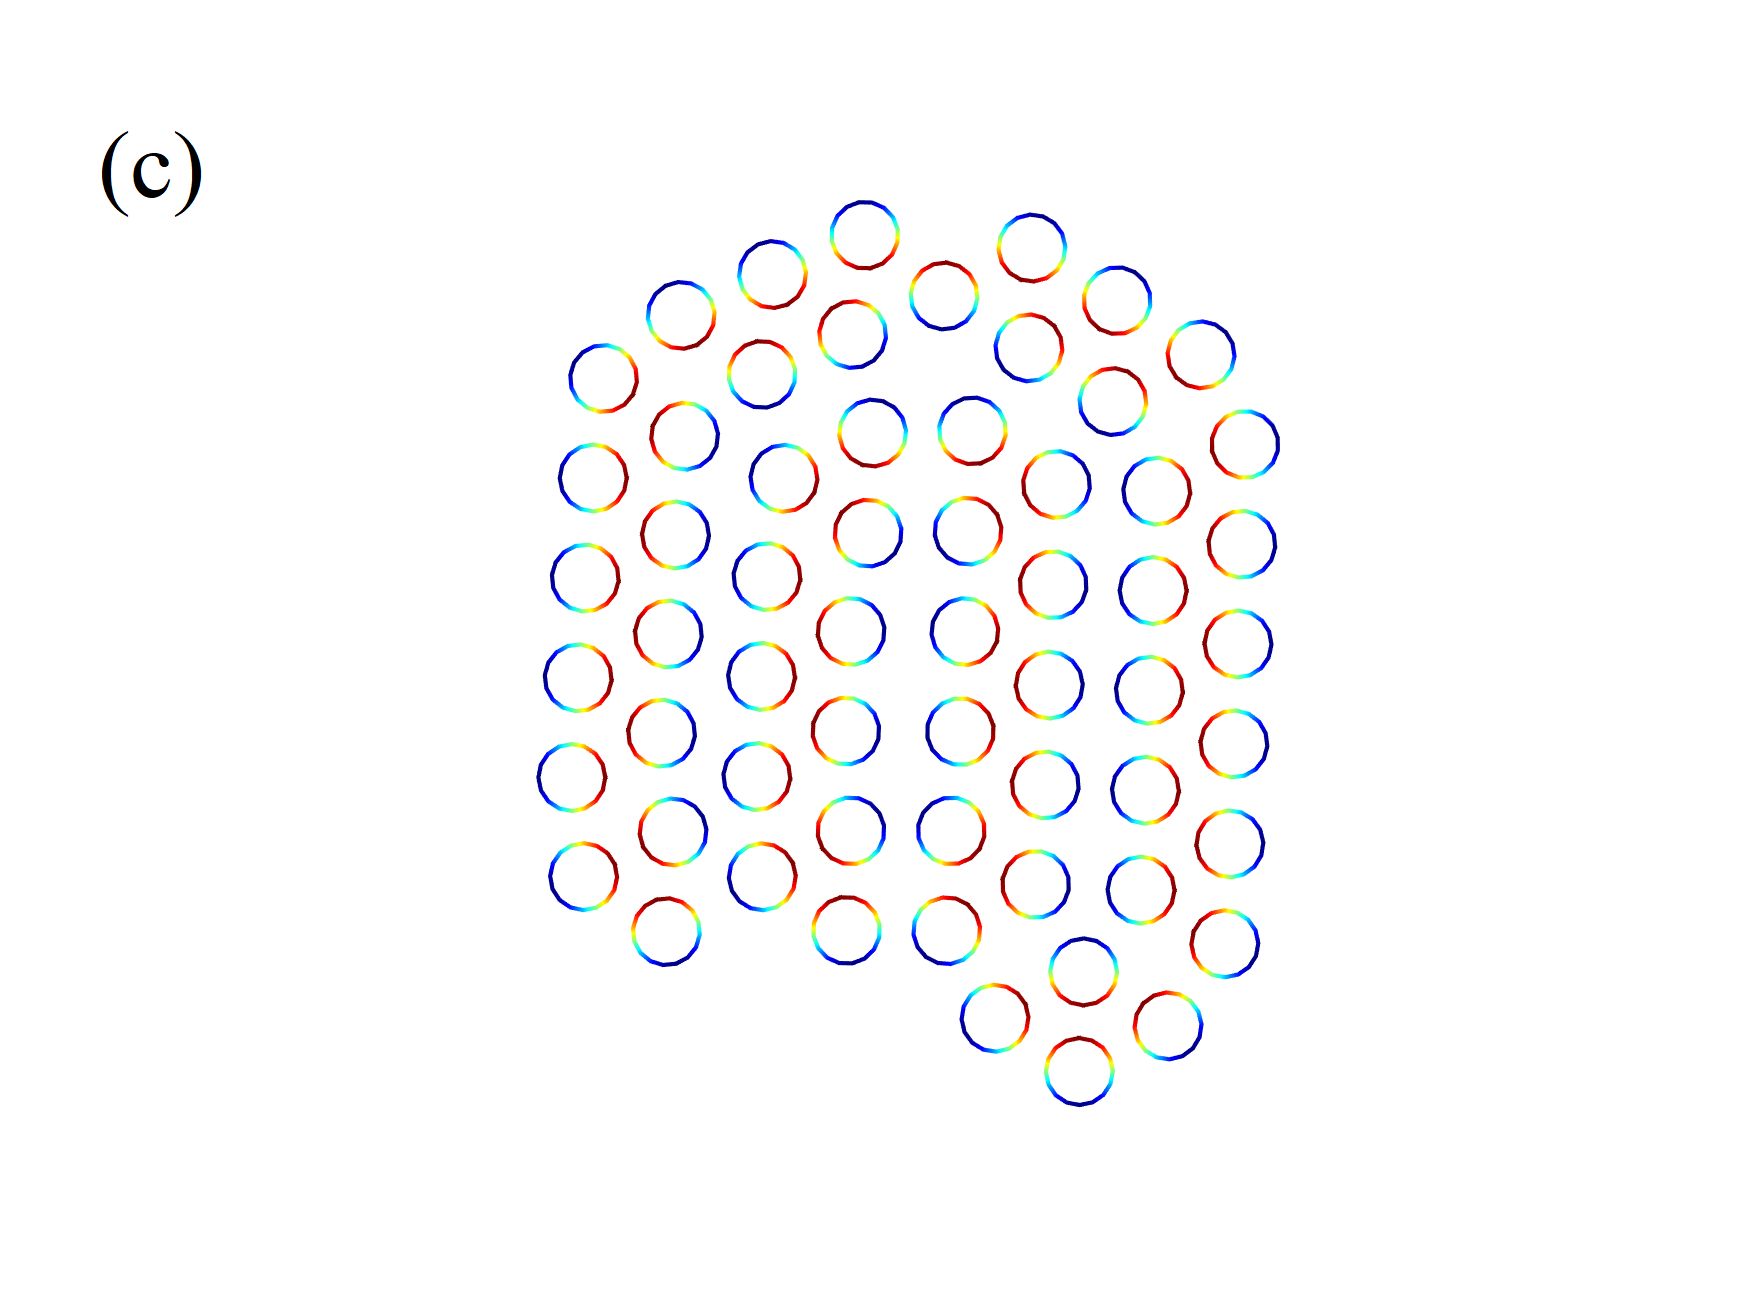
\includegraphics[width=0.4\textwidth]{Fig2c.png}
  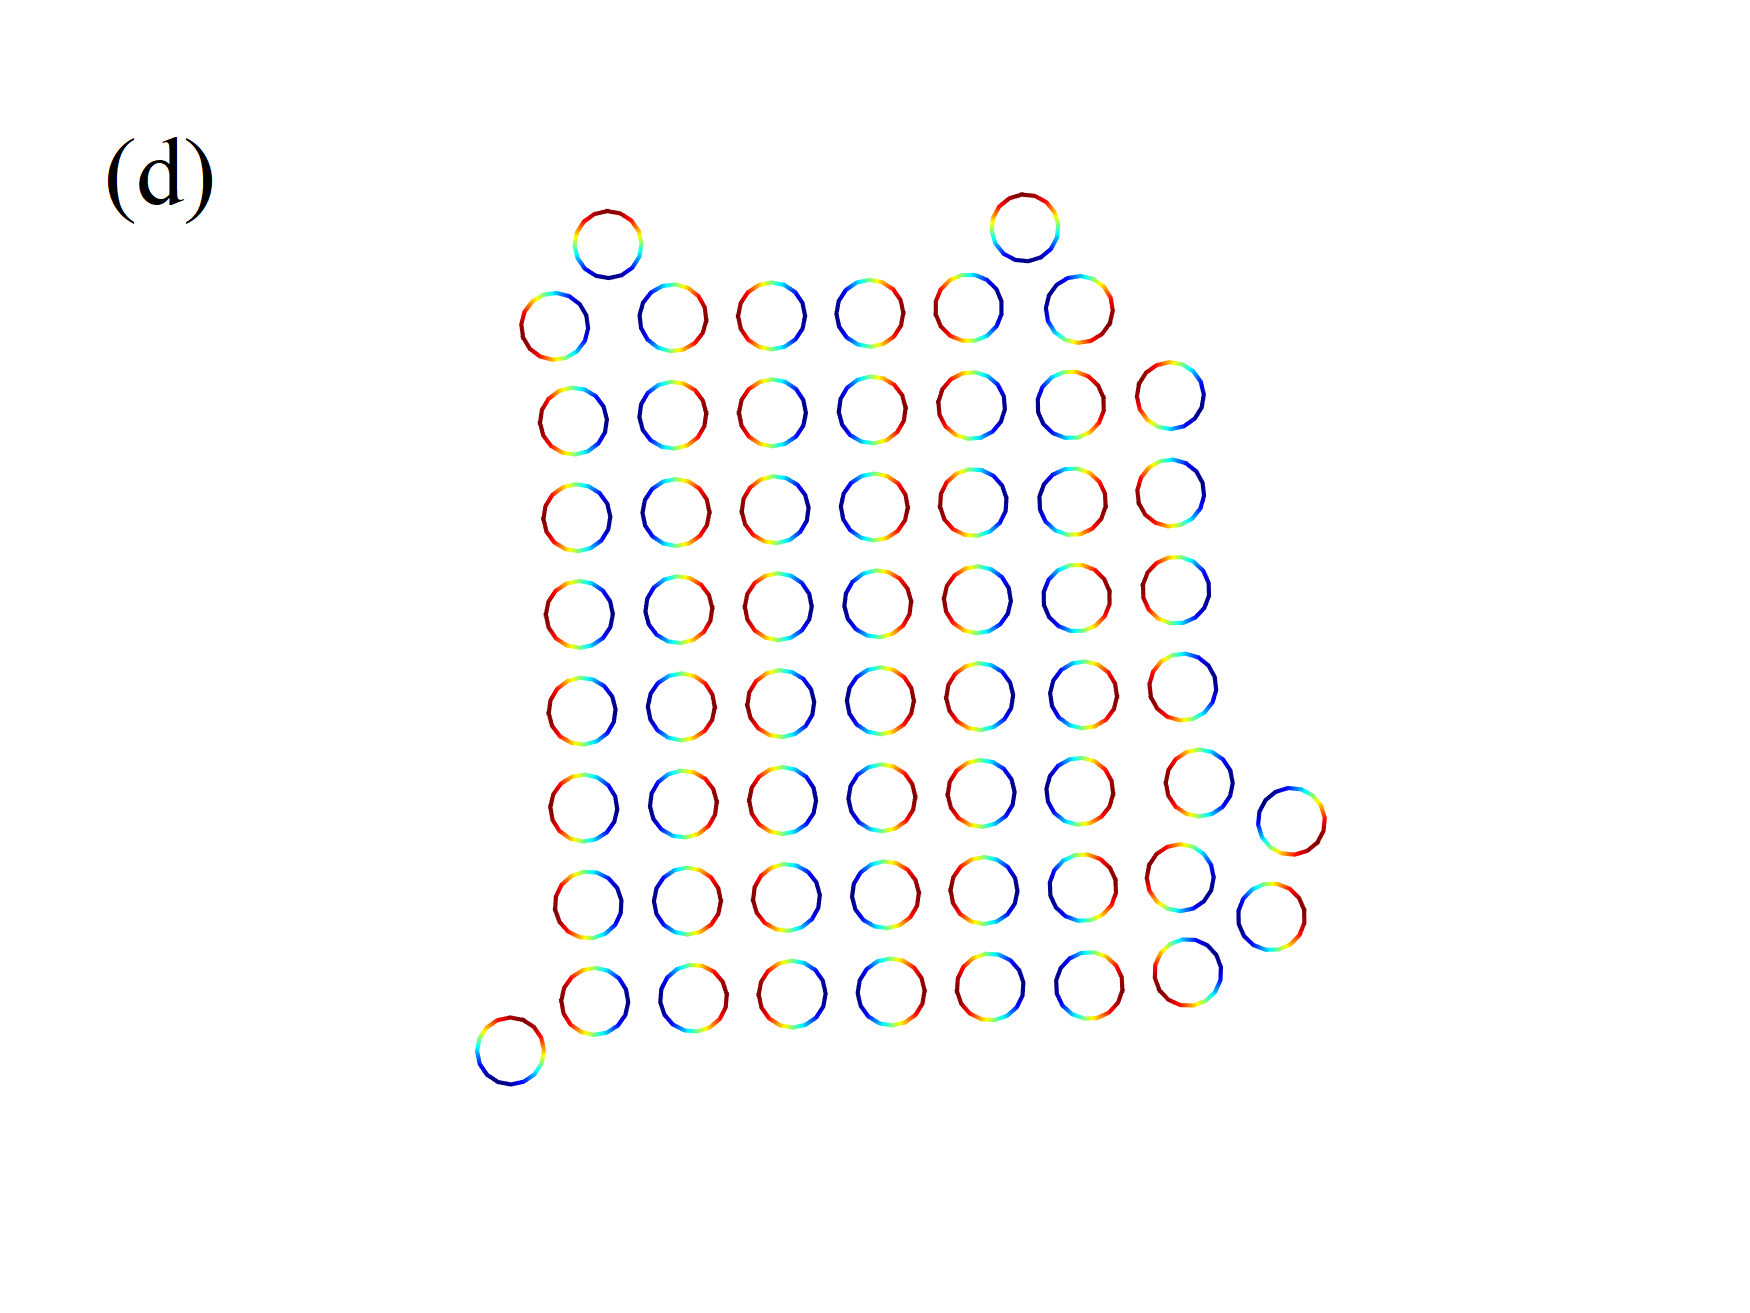
\includegraphics[width=0.4\textwidth]{Fig2d.png}
  \end{center}
  \vspace{-20pt}  
  \caption{\label{fig:relax} (a) Initial configuration for $N_b=60$
  structures. In order to expedite the self-assembly procedure, all
  particles are placed in a $8\times8$ box initially. (b)--(d)
  Equilibrium states for all boundary conditions~\eqref{eq:bcs}(i)--(iii), respectively. Colors represent the boundary values that increases from minimum (blue) to maximum (red).  Panel (b) reaches the equilibrium at $t=1200$; Panel (c) reaches the steady-state at $t=600$; Panel (d) reaches the final state at $t=180$.}
\end{figure}



\begin{figure}
  \begin{center}
  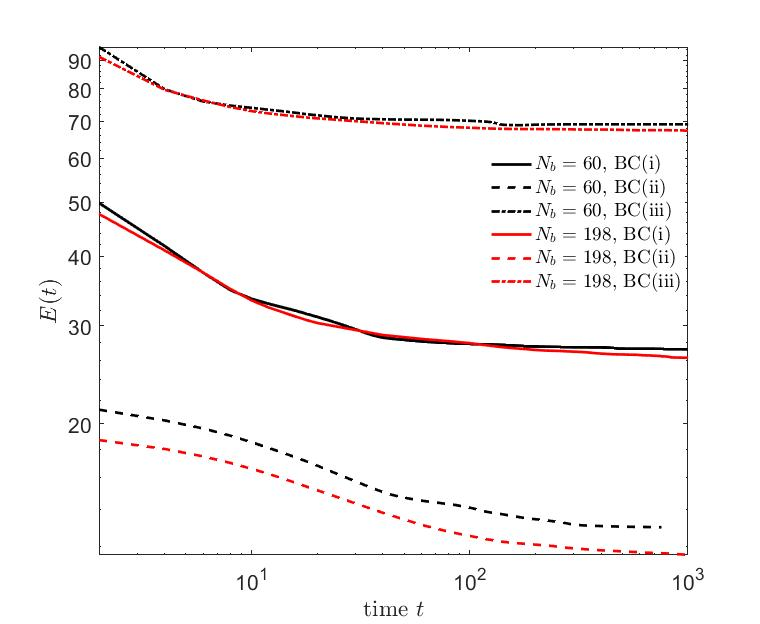
\includegraphics[width=0.5\textwidth]{Relax_Energy.jpg}
  \end{center}
  \vspace{-20pt}  
  \caption{\label{fig:relax_energy} Energy profile for all three boundary conditions.}
\end{figure}

Case (i) models amphiphilic particles.
Amphiphilic particles have a hydrophobic tail and a hydrophilic head
and these are accounted for as follows.
The hydrophilic side takes the value $u =0$.
This mimics the apolar head of a lipid, for example, which does
not alter the structure of adjacent waters. The hydrophobic side
represents hydrocarbons and takes the value 
$u > 0$. The interaction between particles is attractive,
and particles will collectively orient their tails toward
one another. Fig~\ref{fig:relax}(b) demonstrates multiple bilayer structures such as pancake and vesicle shapes.


Multilamelar bilayers arise when both sides of the particle 
are hydrophobic. 
The boundary condition \eqref{eq:bcs}(ii) 
gives a particle with a hydrophobic intensity that is greater
on the $\theta_i = 0$ side than on the $\theta_i = \pi$ side.
The initial self-assembly is similar to that in case (i).
The difference arises in the long-time dynamics where the bilayers
no longer remain well-separated. 
Rather, the bilayers form layers 
as a consequence of the interfacial tension of exposed particle
heads.%~\cite{Huetal19, deMeetal21}. 
Figure~\ref{fig:relax}(c) shows the multilamellar structure with 8
layers when $N_b=60$.  The number of folds depends on several factors,
for instances, number of particles and initial configurations.


Finally, boundary condition \eqref{eq:bcs}(iii) models a particle whose
head surface repels the tail surface as proposed in \cite{MaRa76, Ma77}.
The particles initially form chains with their directors perpendicular
to the length of the chain. The equilibrium structure resembles a
checkerboard pattern where each particle coordinates its head with the
head of three other particles and its tail with the tail of three other
particles. Figure~\ref{fig:relax}(d) gives an example that this boundary
condition results a checker board/stripes equilibrium state.


Fig~\ref{fig:relax_energy} shows the energy profile of boundary conditions (i)--(iii) using 
\eqref{eq:free_energy2} with \eqref{eq:normal_deriv} for normal derivative expression. As expected, for all simulation runs, the total energy of the systems decreases and reaches equilibrium states.



\subsection{Collective Janus Particles Suspended in a Shear Flow}
%%%


Consider placing the equilibrium state of boundary condition \eqref{eq:bcs} (ii) for 60 particles in a shear flow,
\begin{equation}
\uu_\infty(\xx) = \dot\gamma ({\bf e}_y\cdot\xx){\bf e}_x,
\end{equation}
%
where $\dot\gamma$ is the shear rate. Fig~\ref{fig:shear_1} (a)--(c) show the snapshots of simulation results when $\dot\gamma=0.05$.
We measure the ratio of major and minor axes $\lambda$ by adopting an ellipse fitting using the singular value decomposition and track this aspect ratio for this multilamellar structure when the flow is on. 
The result is shown in panel (d) and we observe that the multilamellar structure will be slightly stretched and the aspect ratio $\lambda=3.5$ increases over time.
%
Notice that for this simulation, the center of mass position of the
initial configuration is not at the origin and it is slightly to the
right of the origin. We also track the aspect ratio $\lambda$ for the
case that the center of mass position is shifted to the origin. Panel
(d) also shows that the dynamics of two sets of simulations are
invariant of center of mass position in a shear flow.

%
\begin{figure}
  \begin{center}
  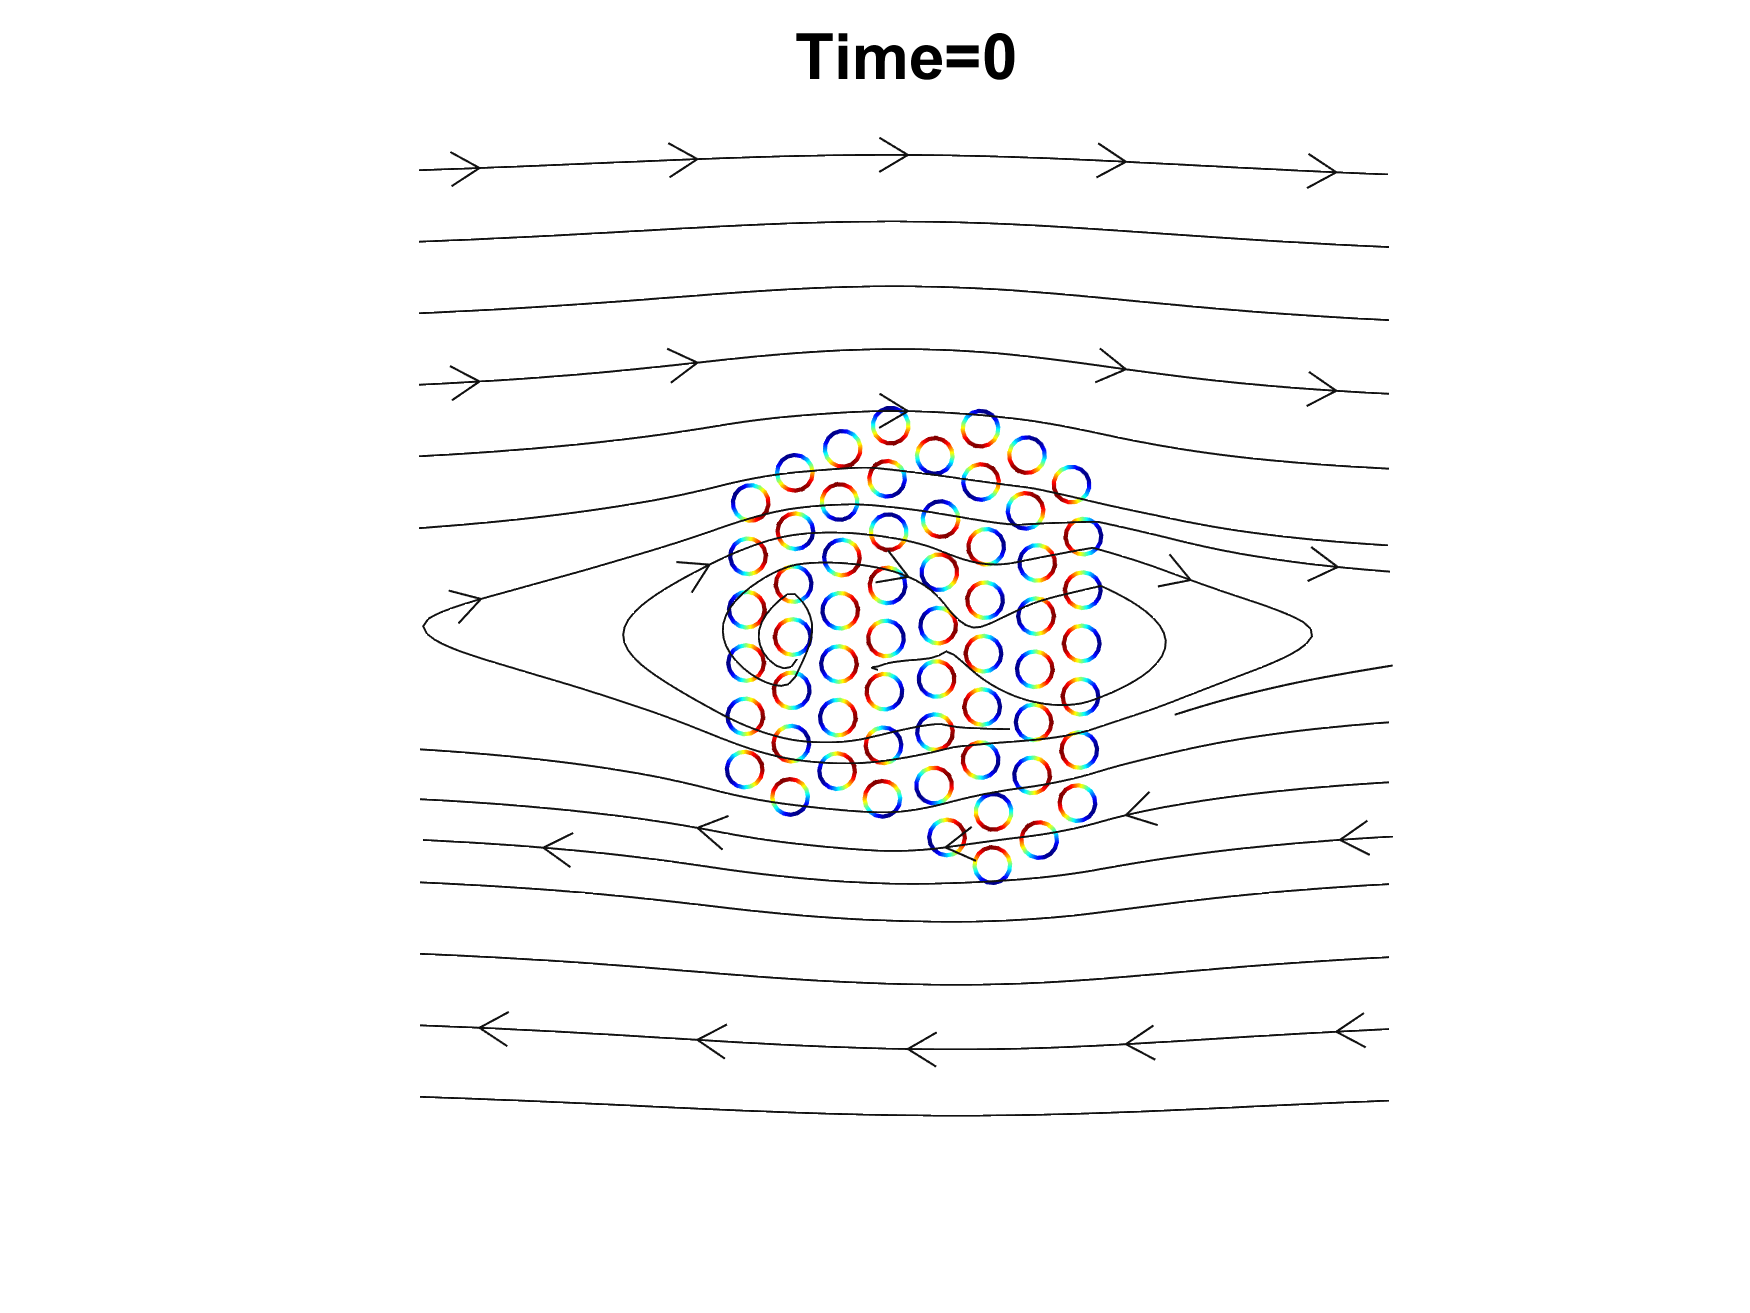
\includegraphics[width=0.21\textwidth]{shear_0.png}
  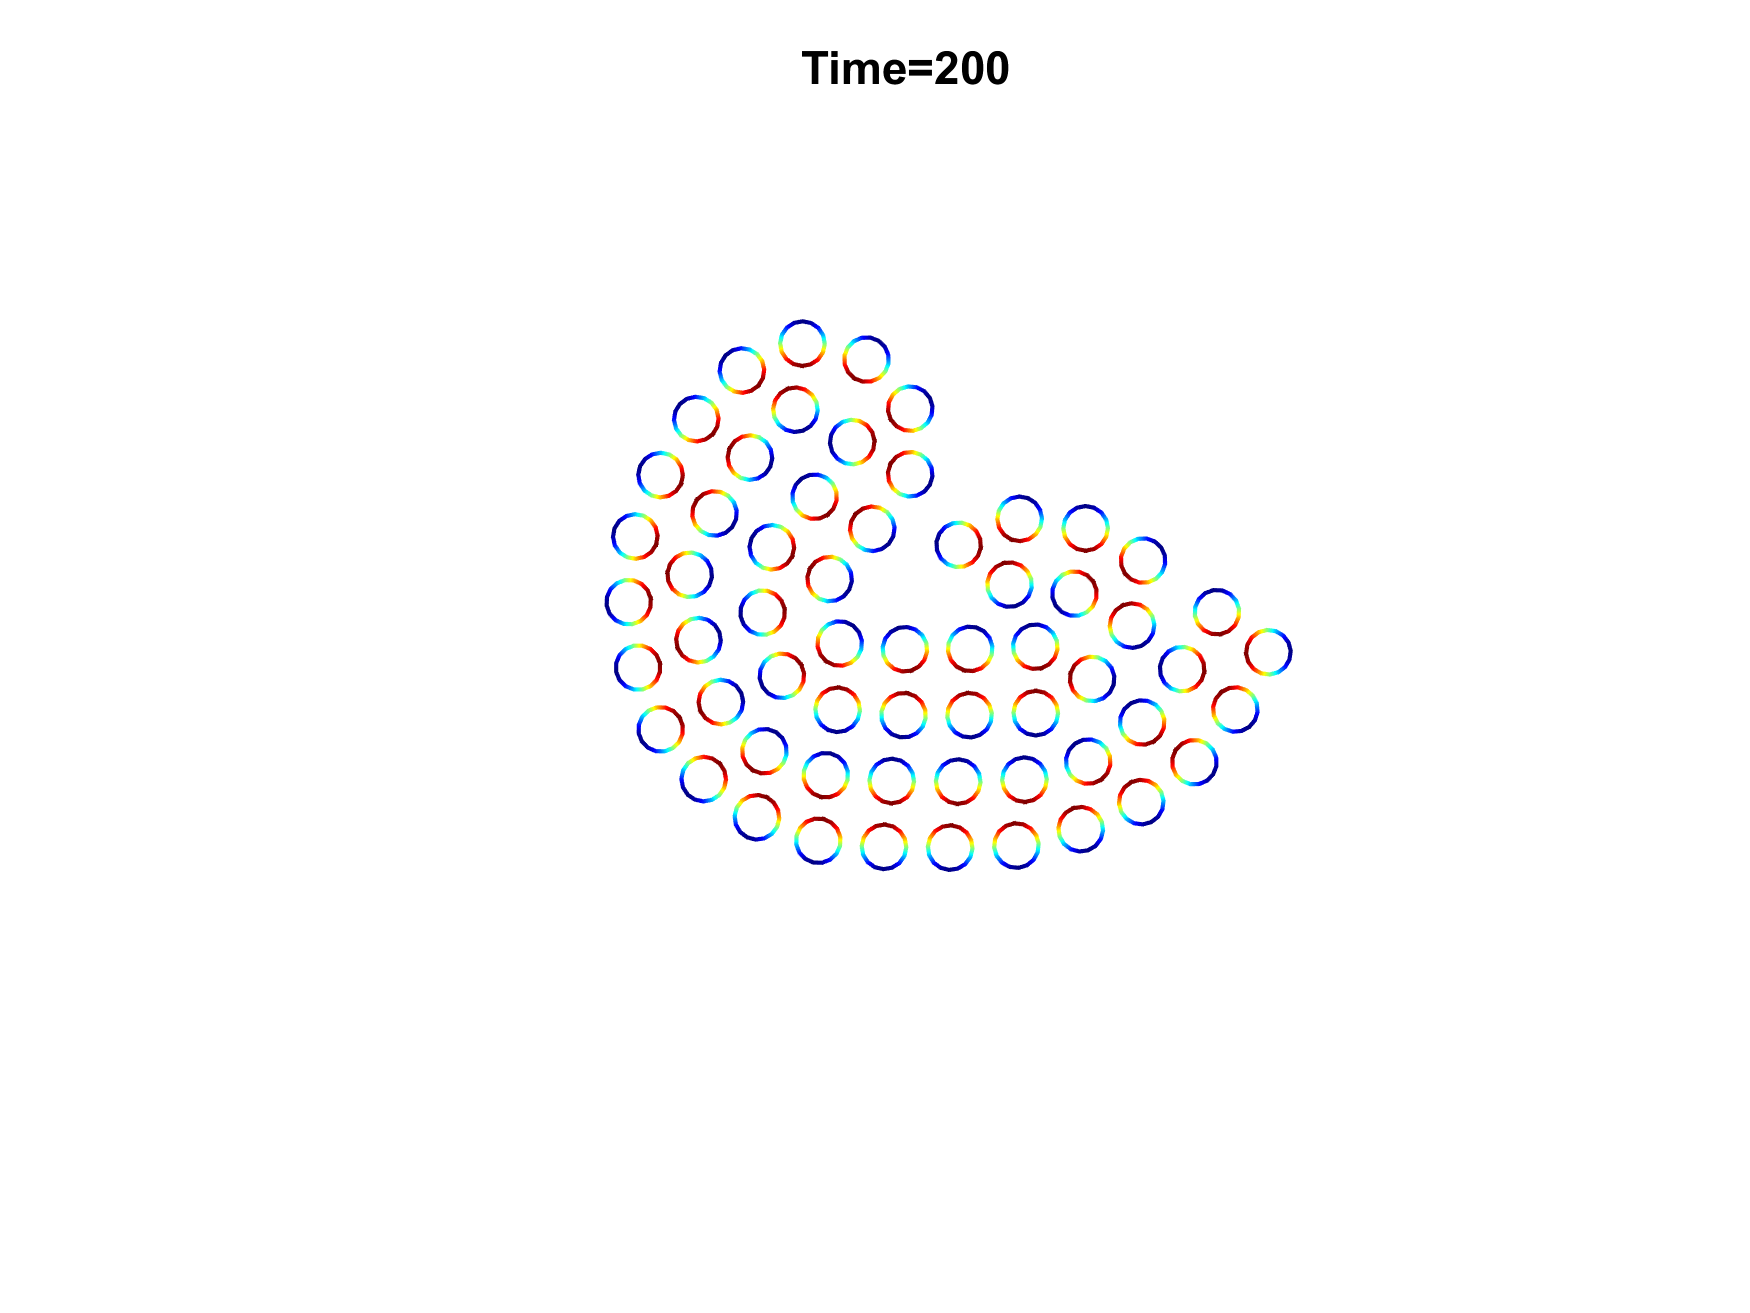
\includegraphics[width=0.21\textwidth]{shear_1000.png}
  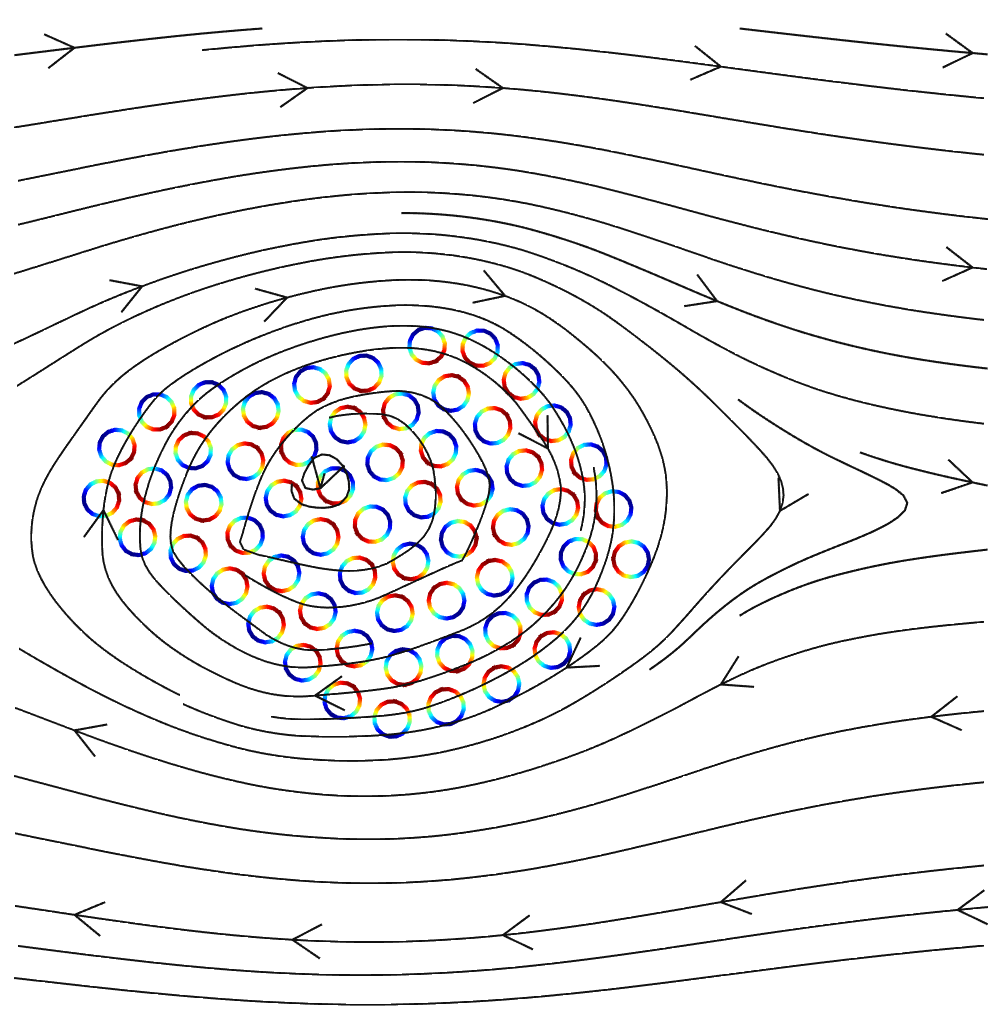
\includegraphics[width=0.21\textwidth]{shear_2000.png} 
  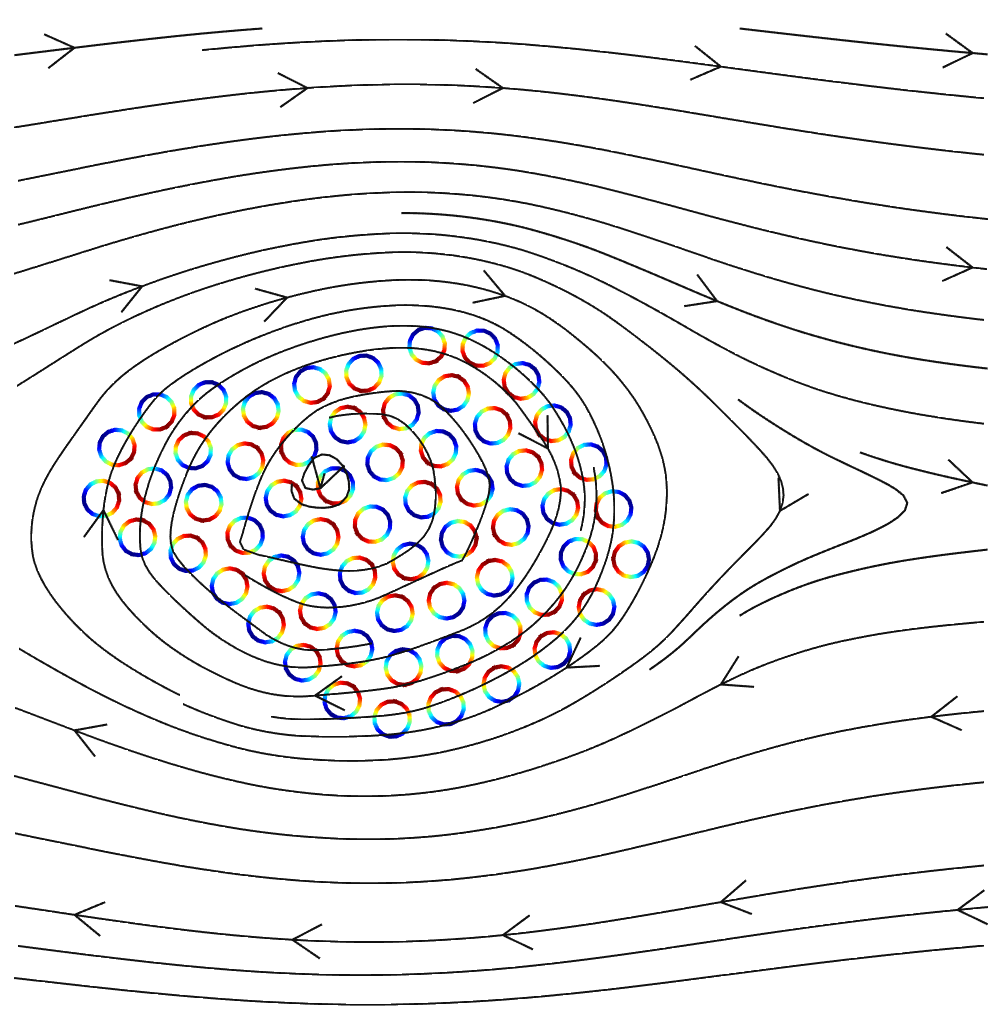
\includegraphics[width=0.21\textwidth]{shear_2000.png} \\
  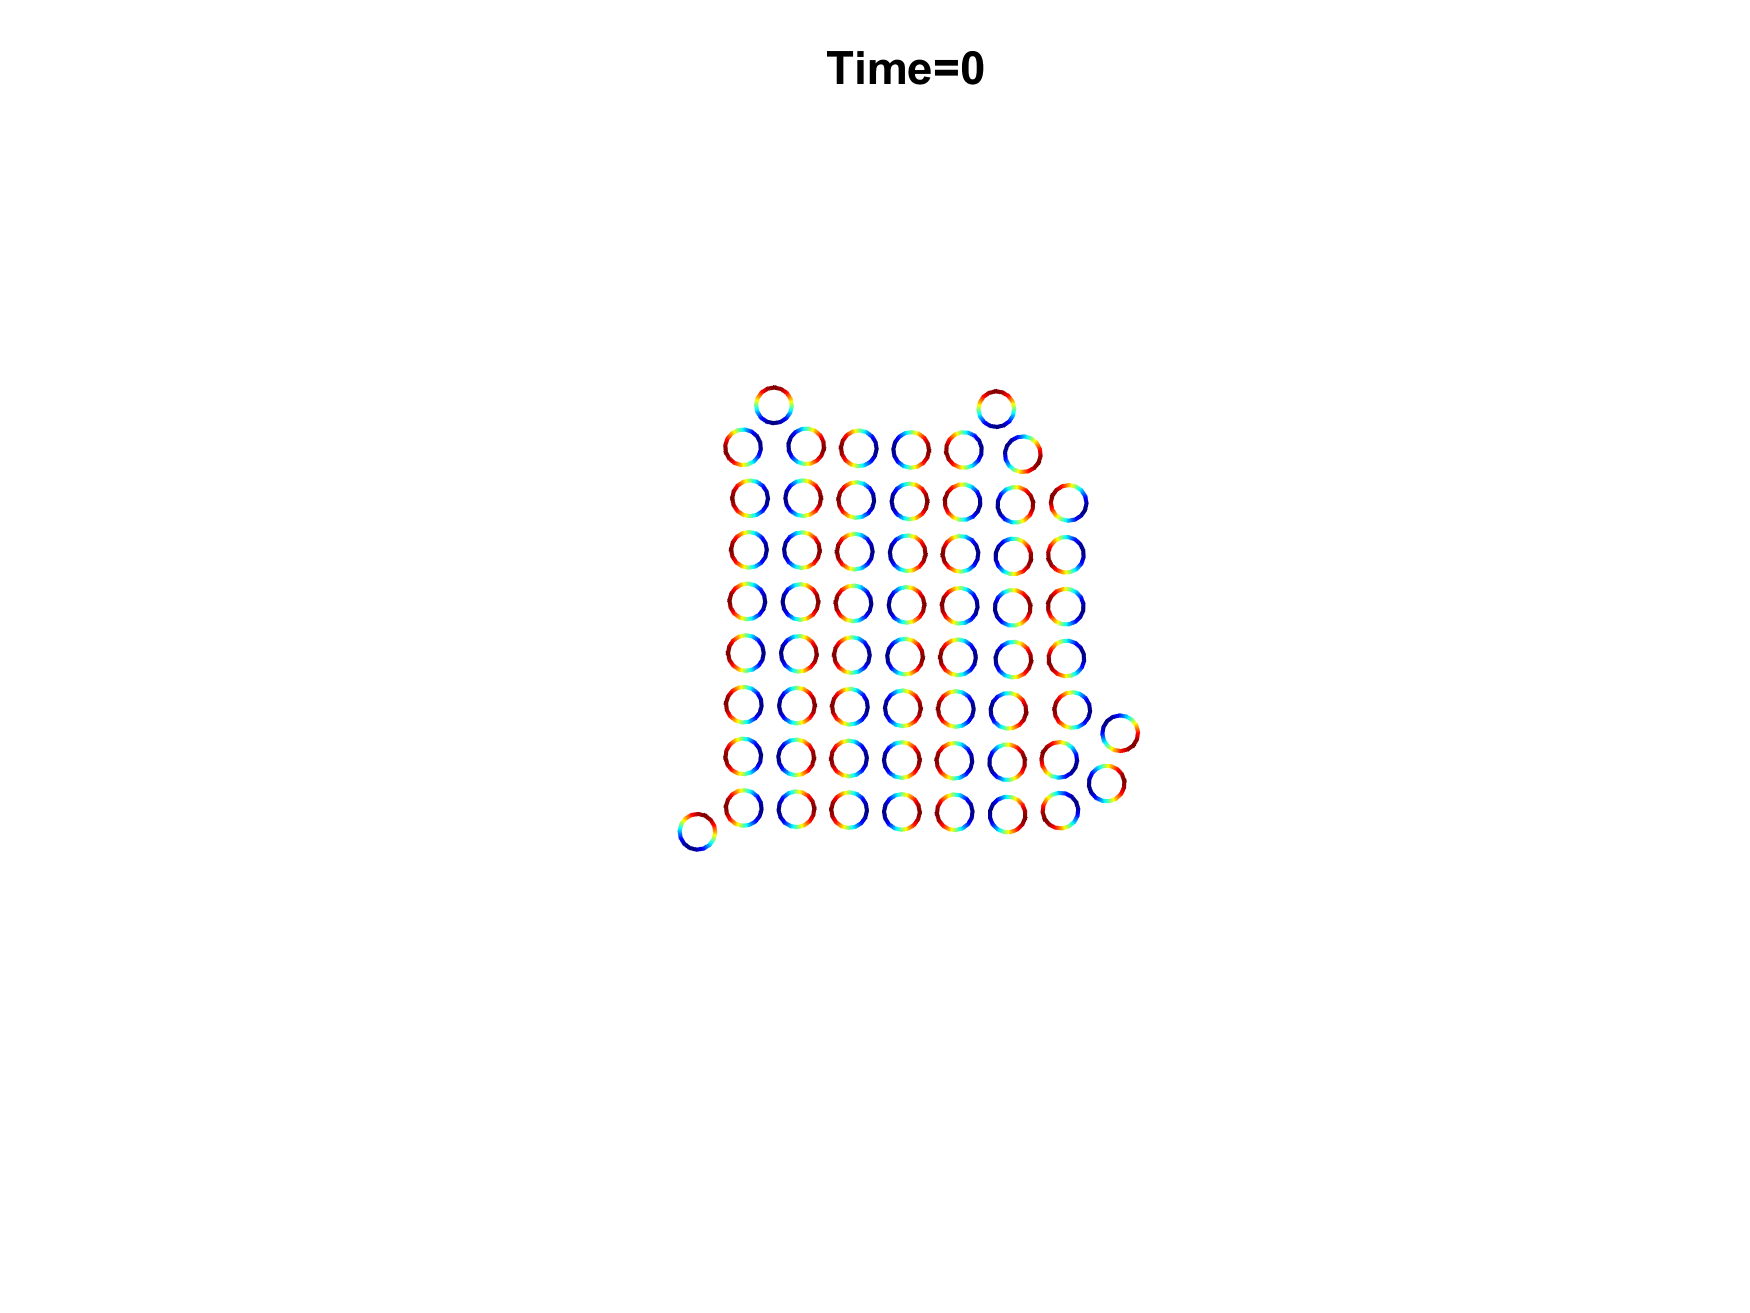
\includegraphics[width=0.21\textwidth]{shear_checker_0.png}
  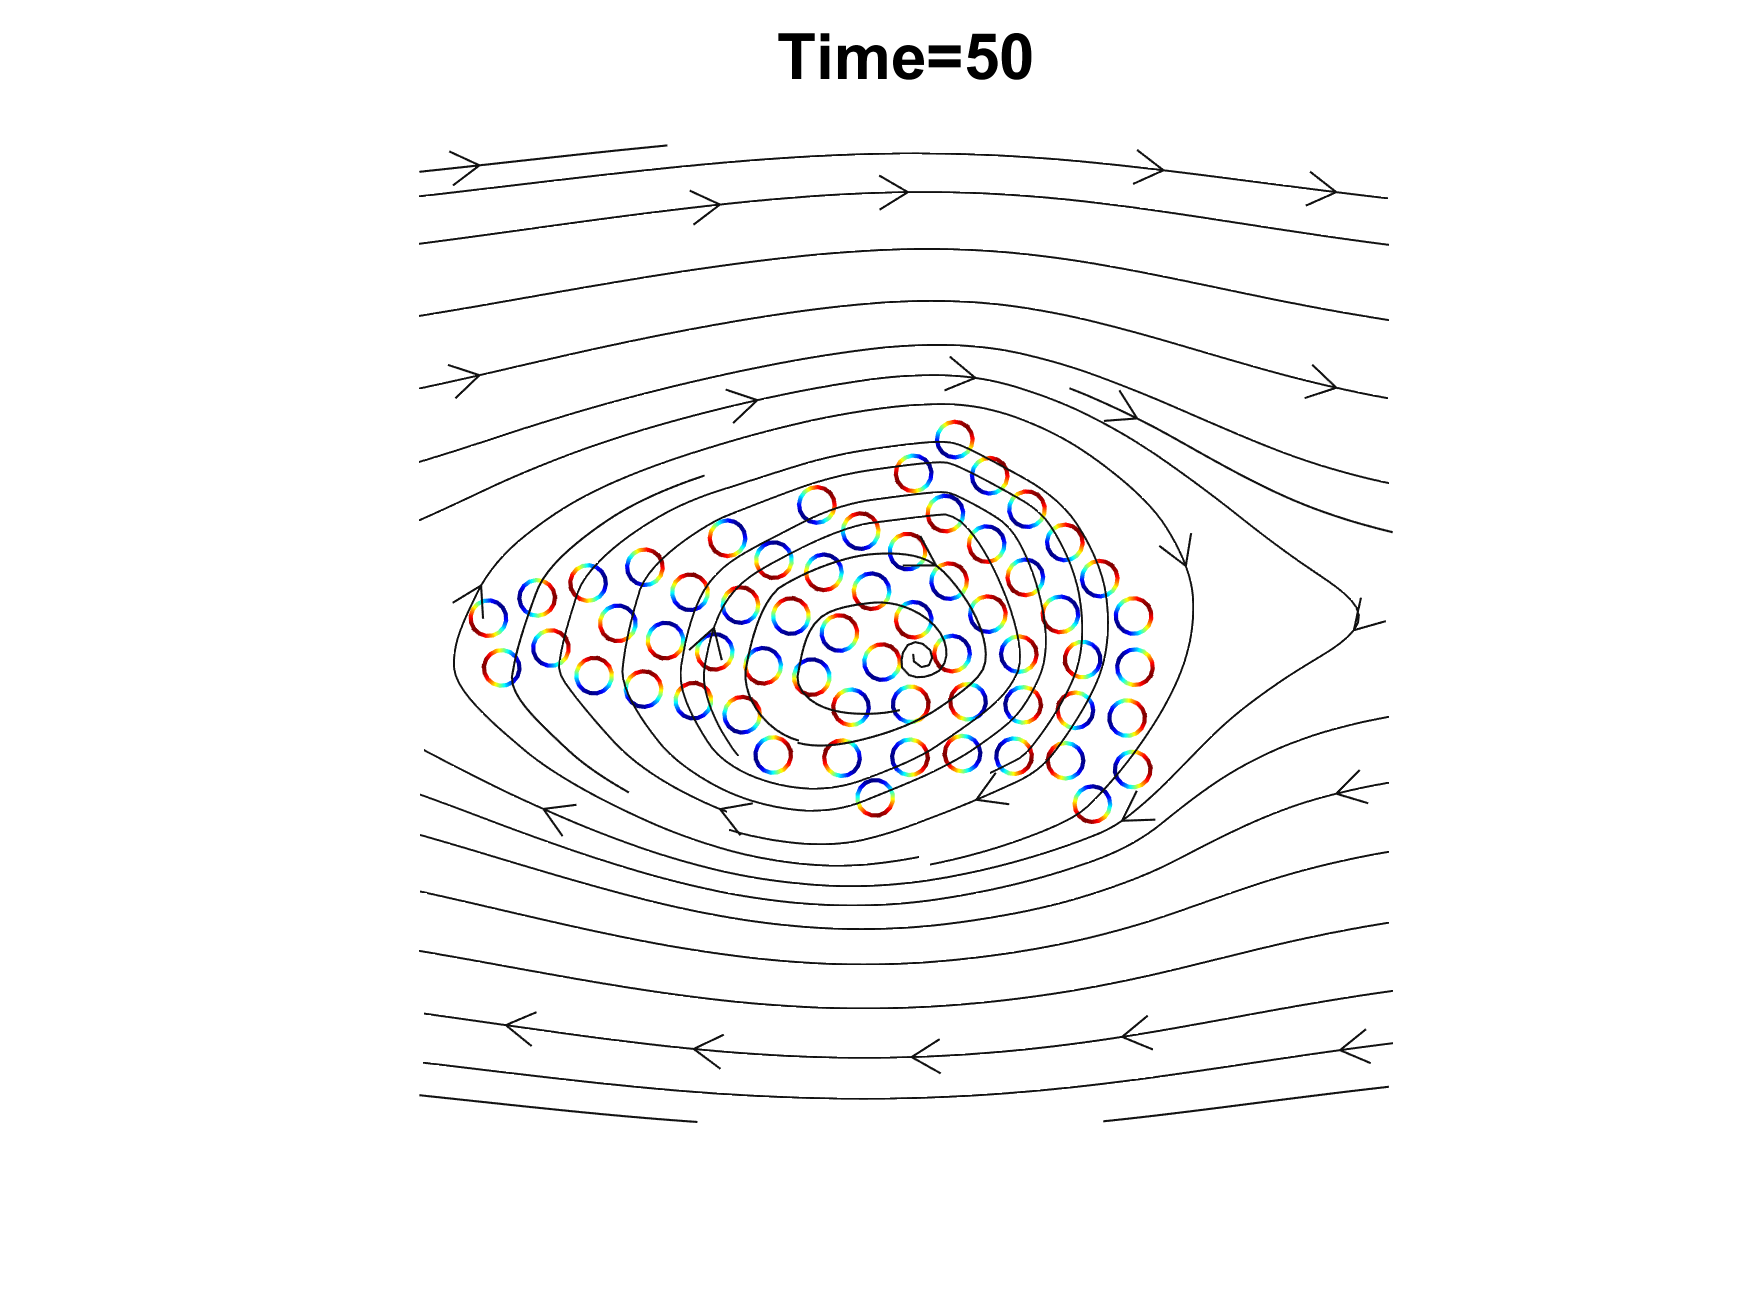
\includegraphics[width=0.21\textwidth]{shear_checker_250.png}
  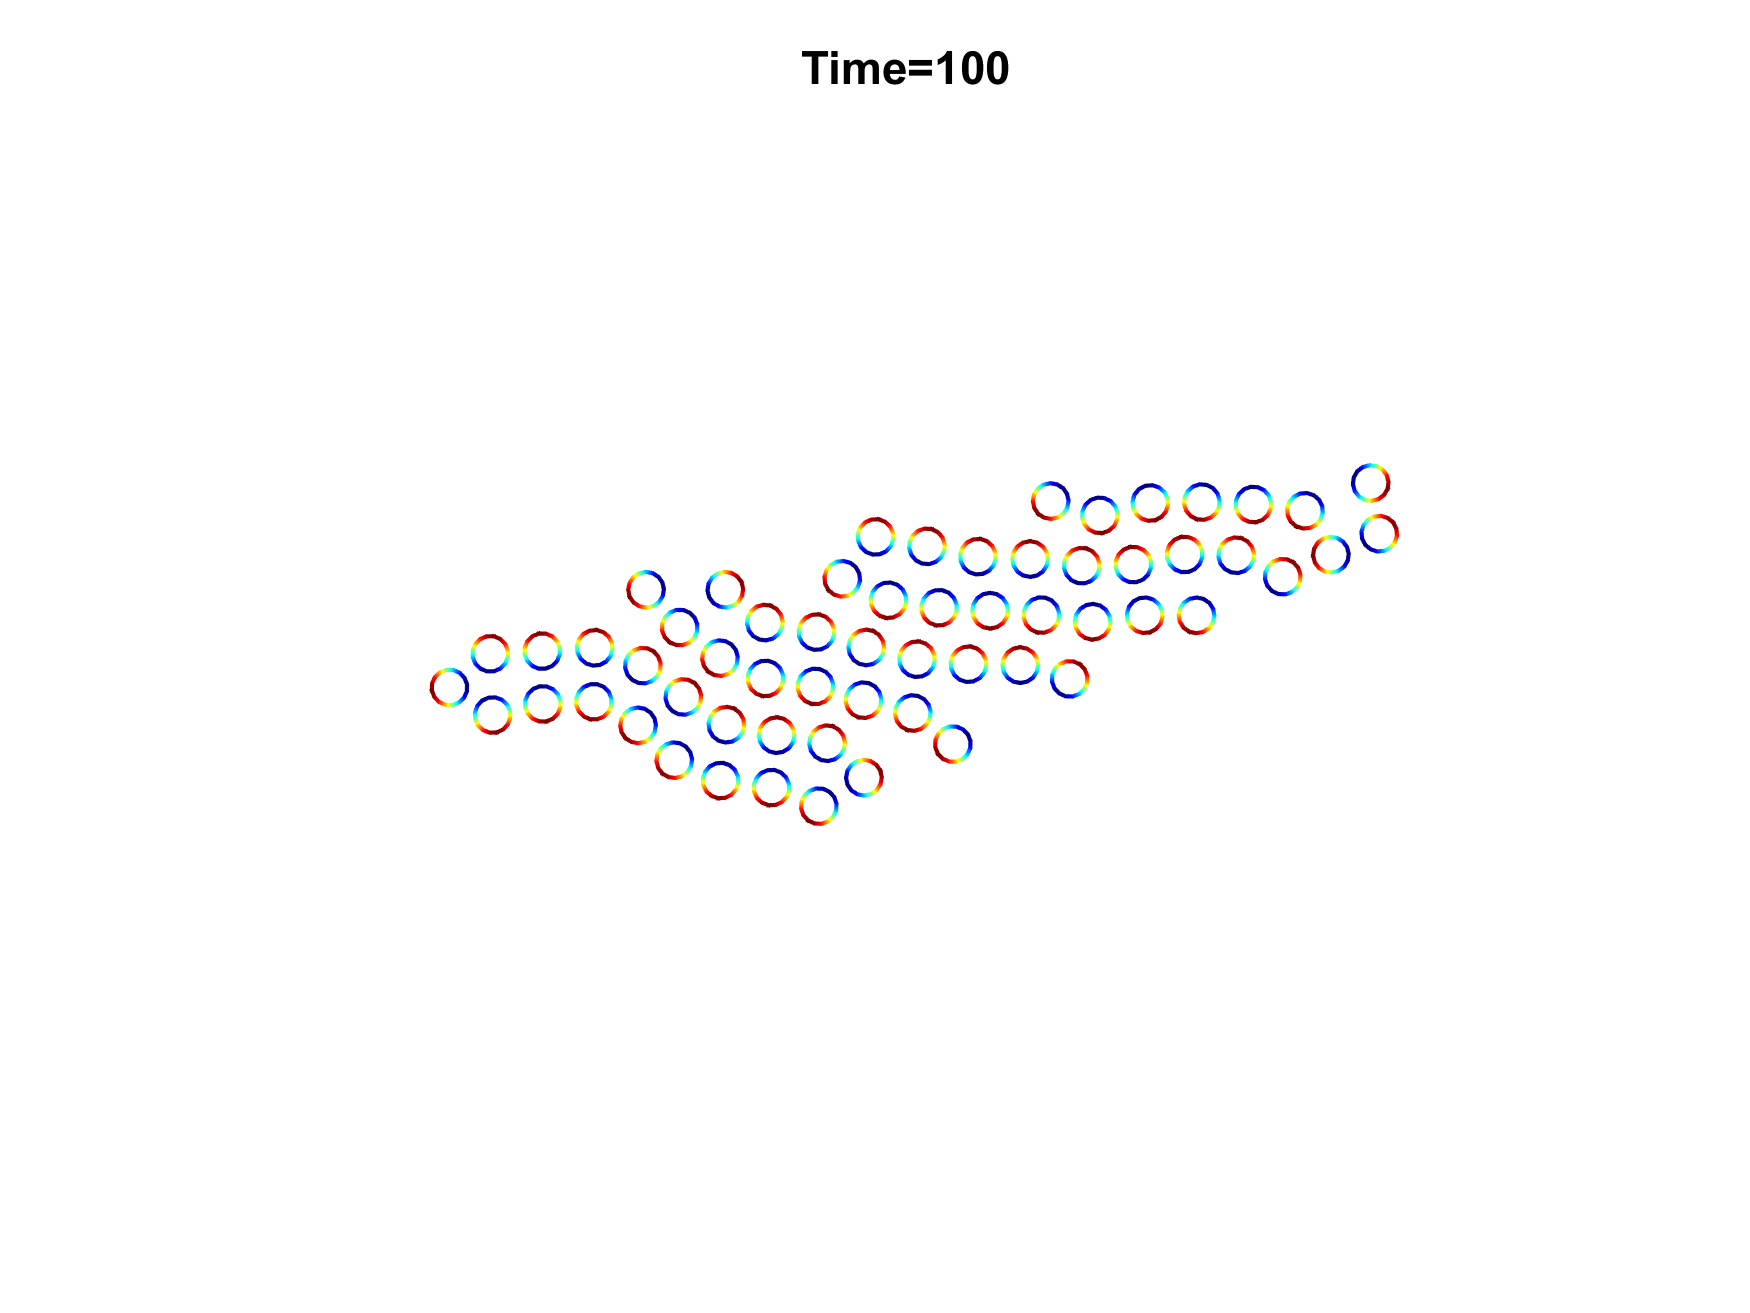
\includegraphics[width=0.21\textwidth]{shear_checker_500.png}
  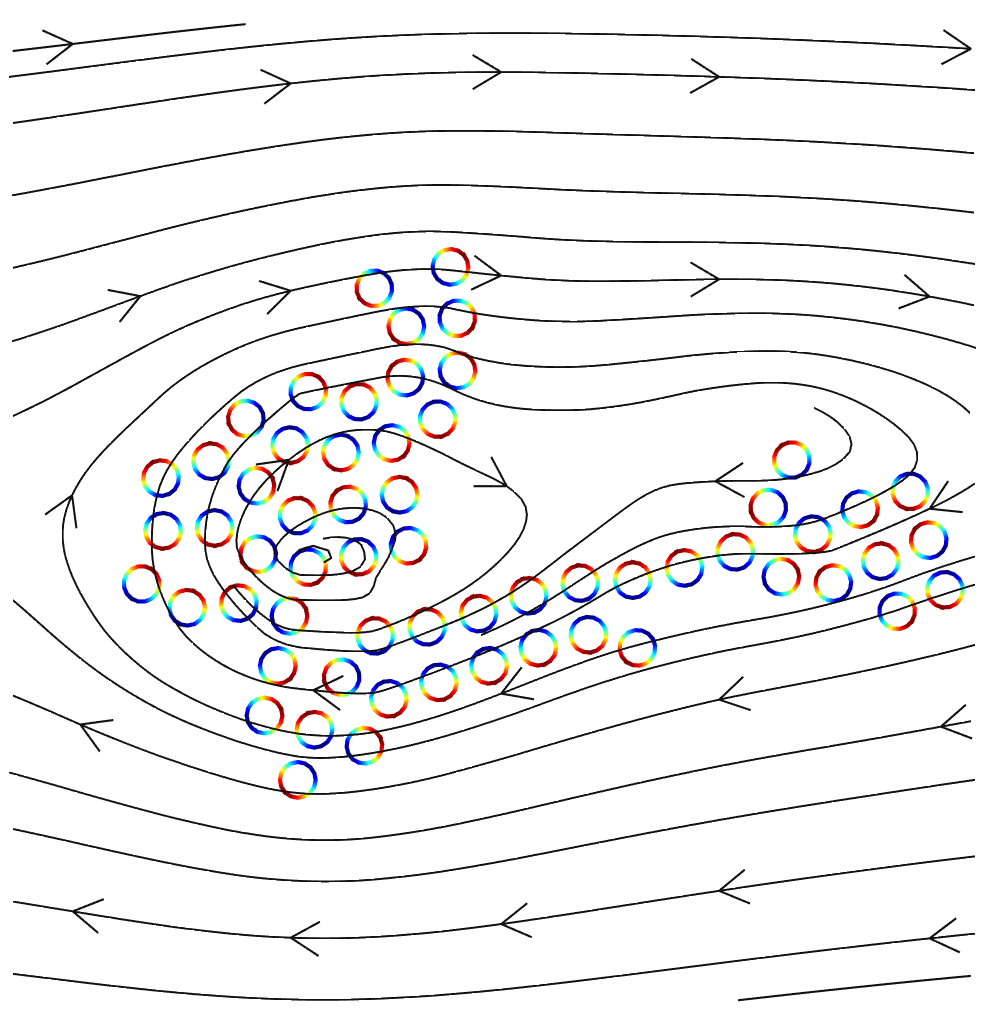
\includegraphics[width=0.21\textwidth]{shear_checker_750.png} \\
  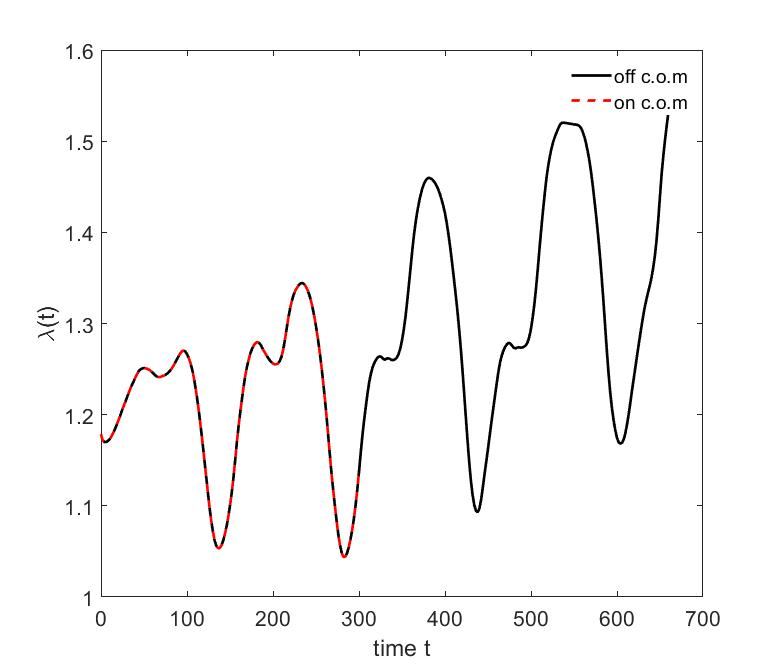
\includegraphics[width=0.4\textwidth]{lambda_fig1.jpg}
  \end{center}
  \vspace{-20pt}  
  \caption{\label{fig:shear_1} Snapshots of simulation using boundary condition \eqref{eq:bcs}(ii) in a shear flow when $\dot\gamma=0.05$. }
\end{figure}
%

%Consider the energy profiles for two simulations where the centor of mass is on and off the origin.
%Fig~\ref{fig:shear_energy1} shows numerical results for both energy profiles and magnitude of energy differences is significantly large when there is a large deformation, for instance, the case when a multi-lamellar structure deformed to a pancake shape.
%
%\begin{figure}
%  \begin{center}
%  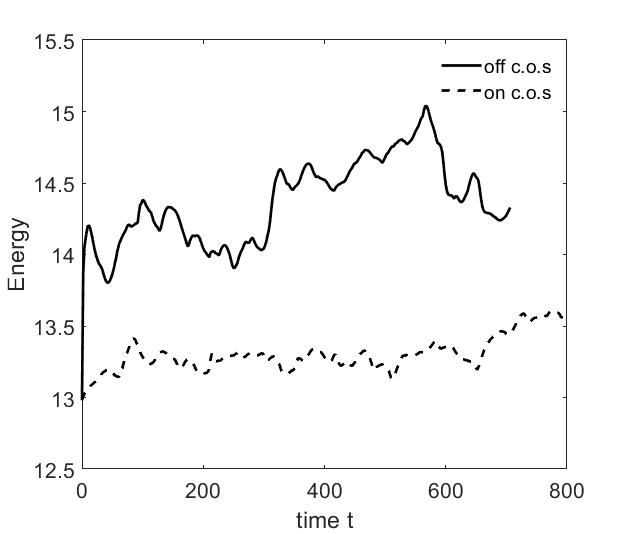
\includegraphics[width=0.5\textwidth]{shear_energy1.jpg}
%  \end{center}
%  \vspace{-20pt}  
%  \caption{\label{fig:shear_energy1} Energy profiles tracked during the simulations using boundary condition \eqref{eq:bcs}(ii) in a shear flow when $\dot\gamma=0.05$. }
%\end{figure}




%%%

The second set of simulation is putting the equilibrium state of the
boundary condition \eqref{eq:bcs} (iii), the checker board, in a shear
flow. After a set of empirical numerical investigations, we obtain a
critical shear rate $\dot\gamma=0.15$ where the checker board deforms
into stripes and small groups of JP. Figure~\ref{fig:shear_2}(a)--(d) show configurations when $t=\{0,50,100,150\}$. %The deformation starts with stripe separations
%
%\begin{figure}
%  \begin{center}
%  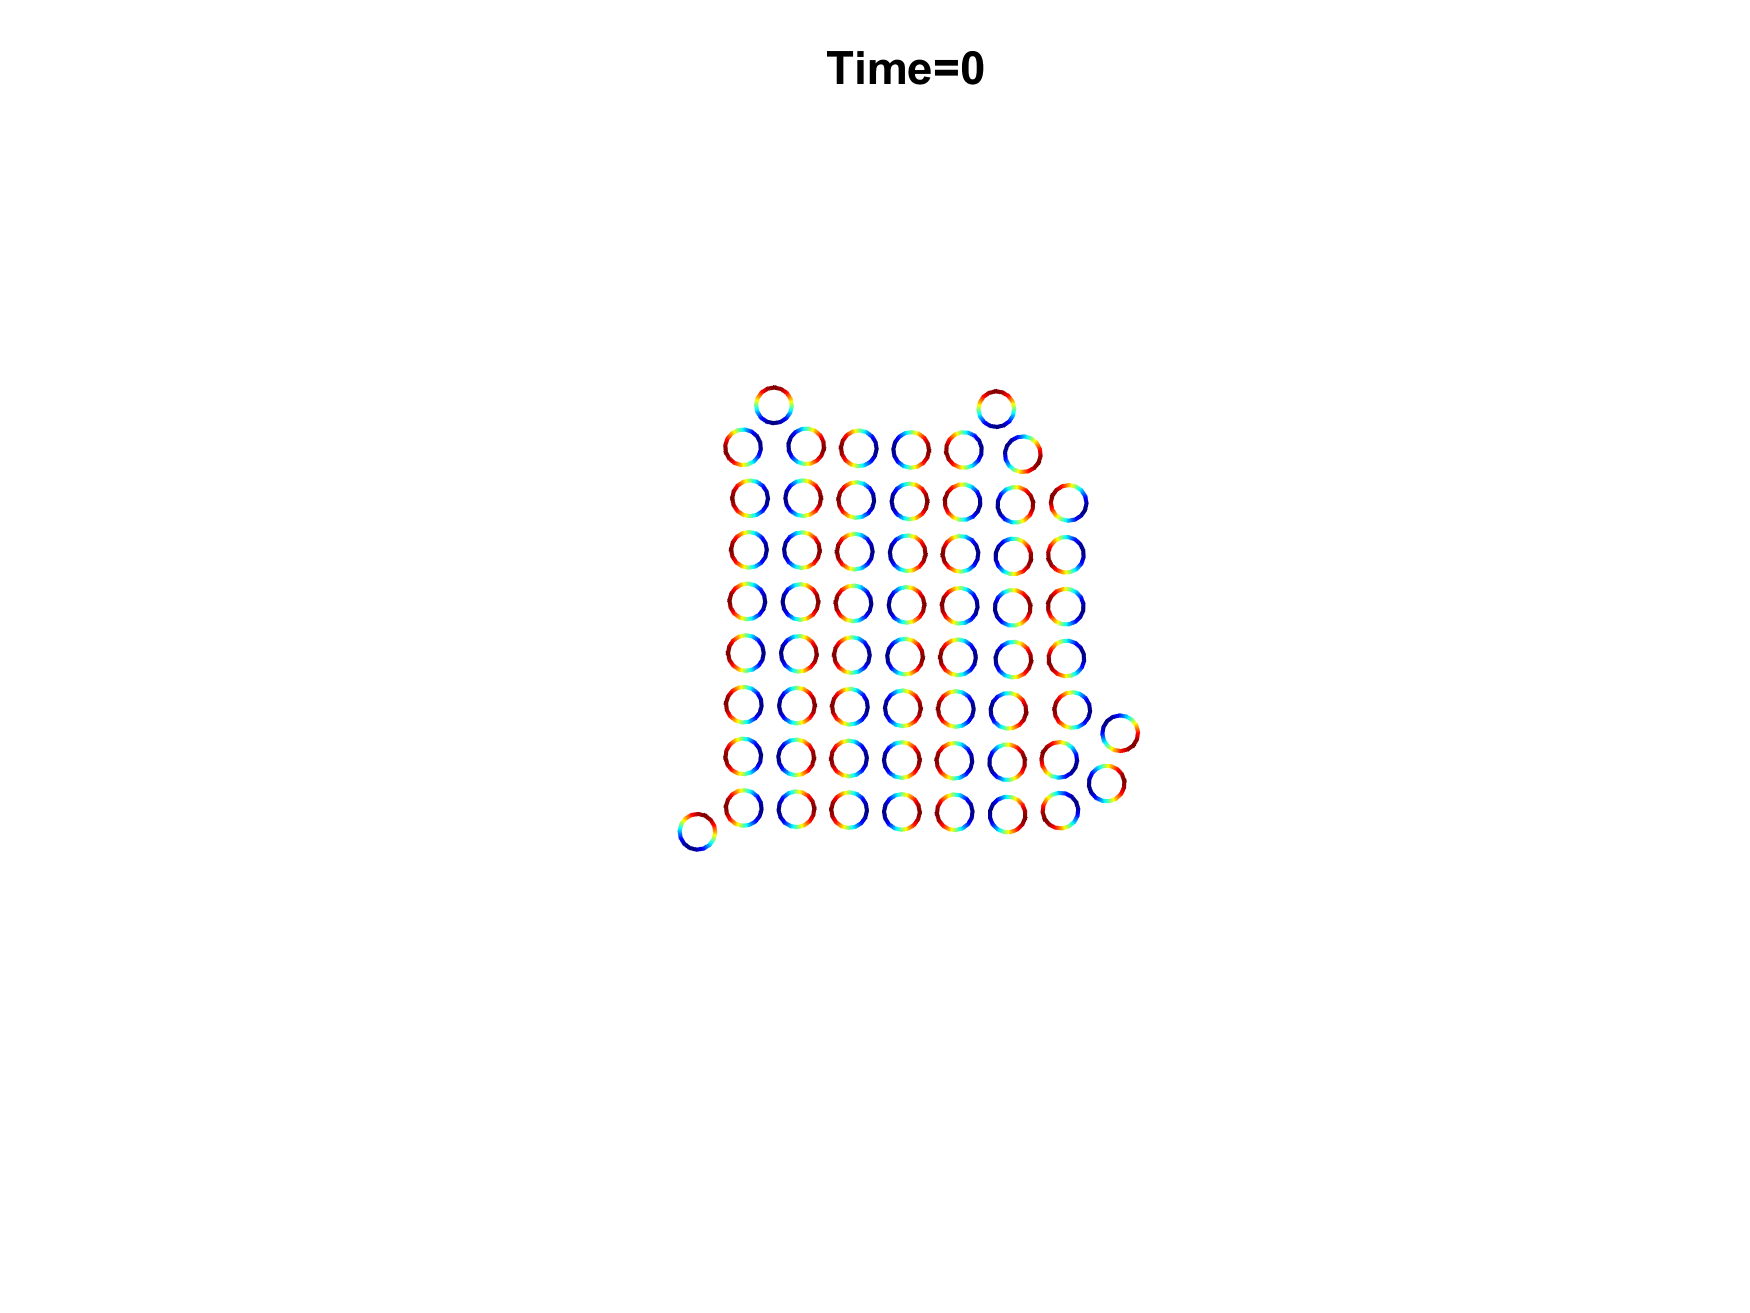
\includegraphics[width=0.4\textwidth]{shear_checker_0.png}
%  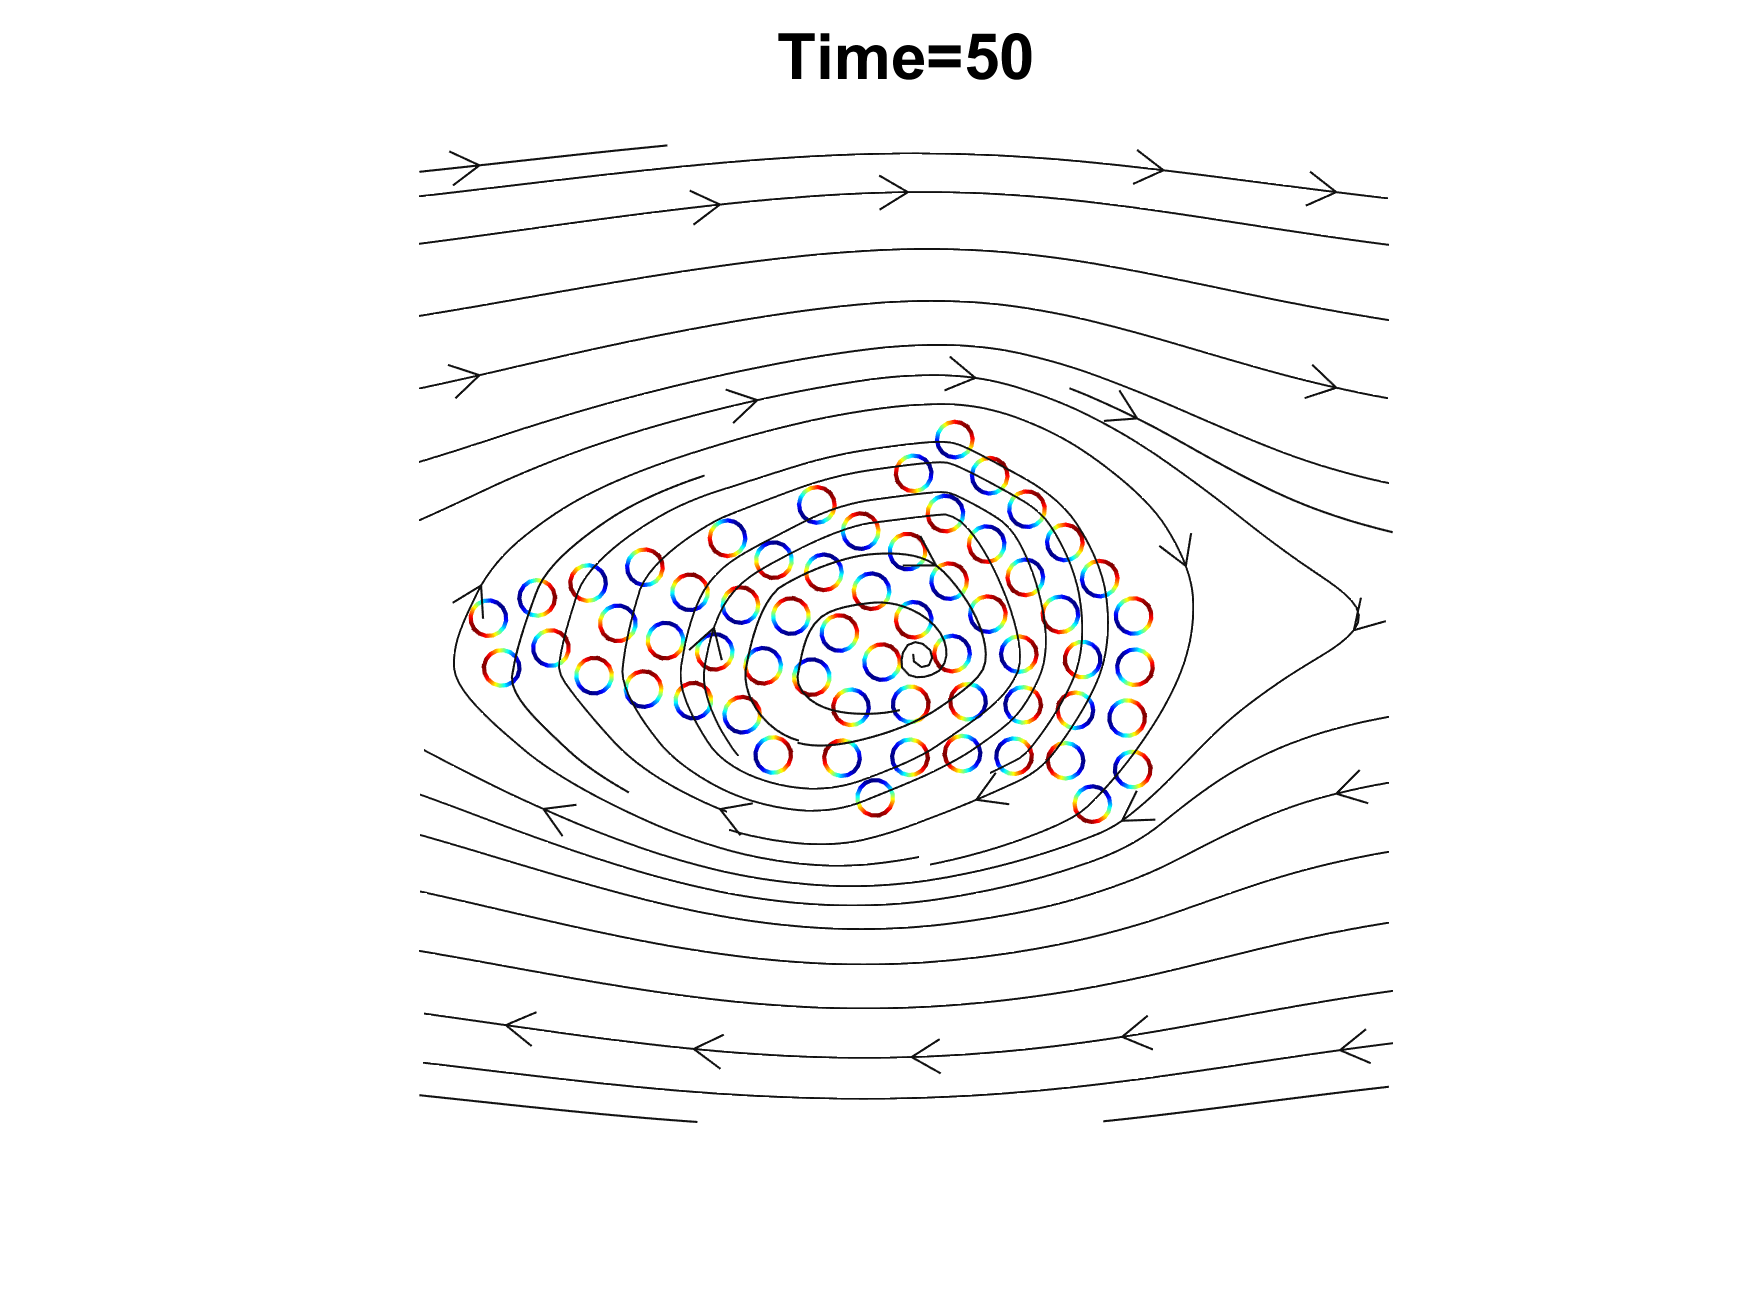
\includegraphics[width=0.4\textwidth]{shear_checker_250.png}\\
%  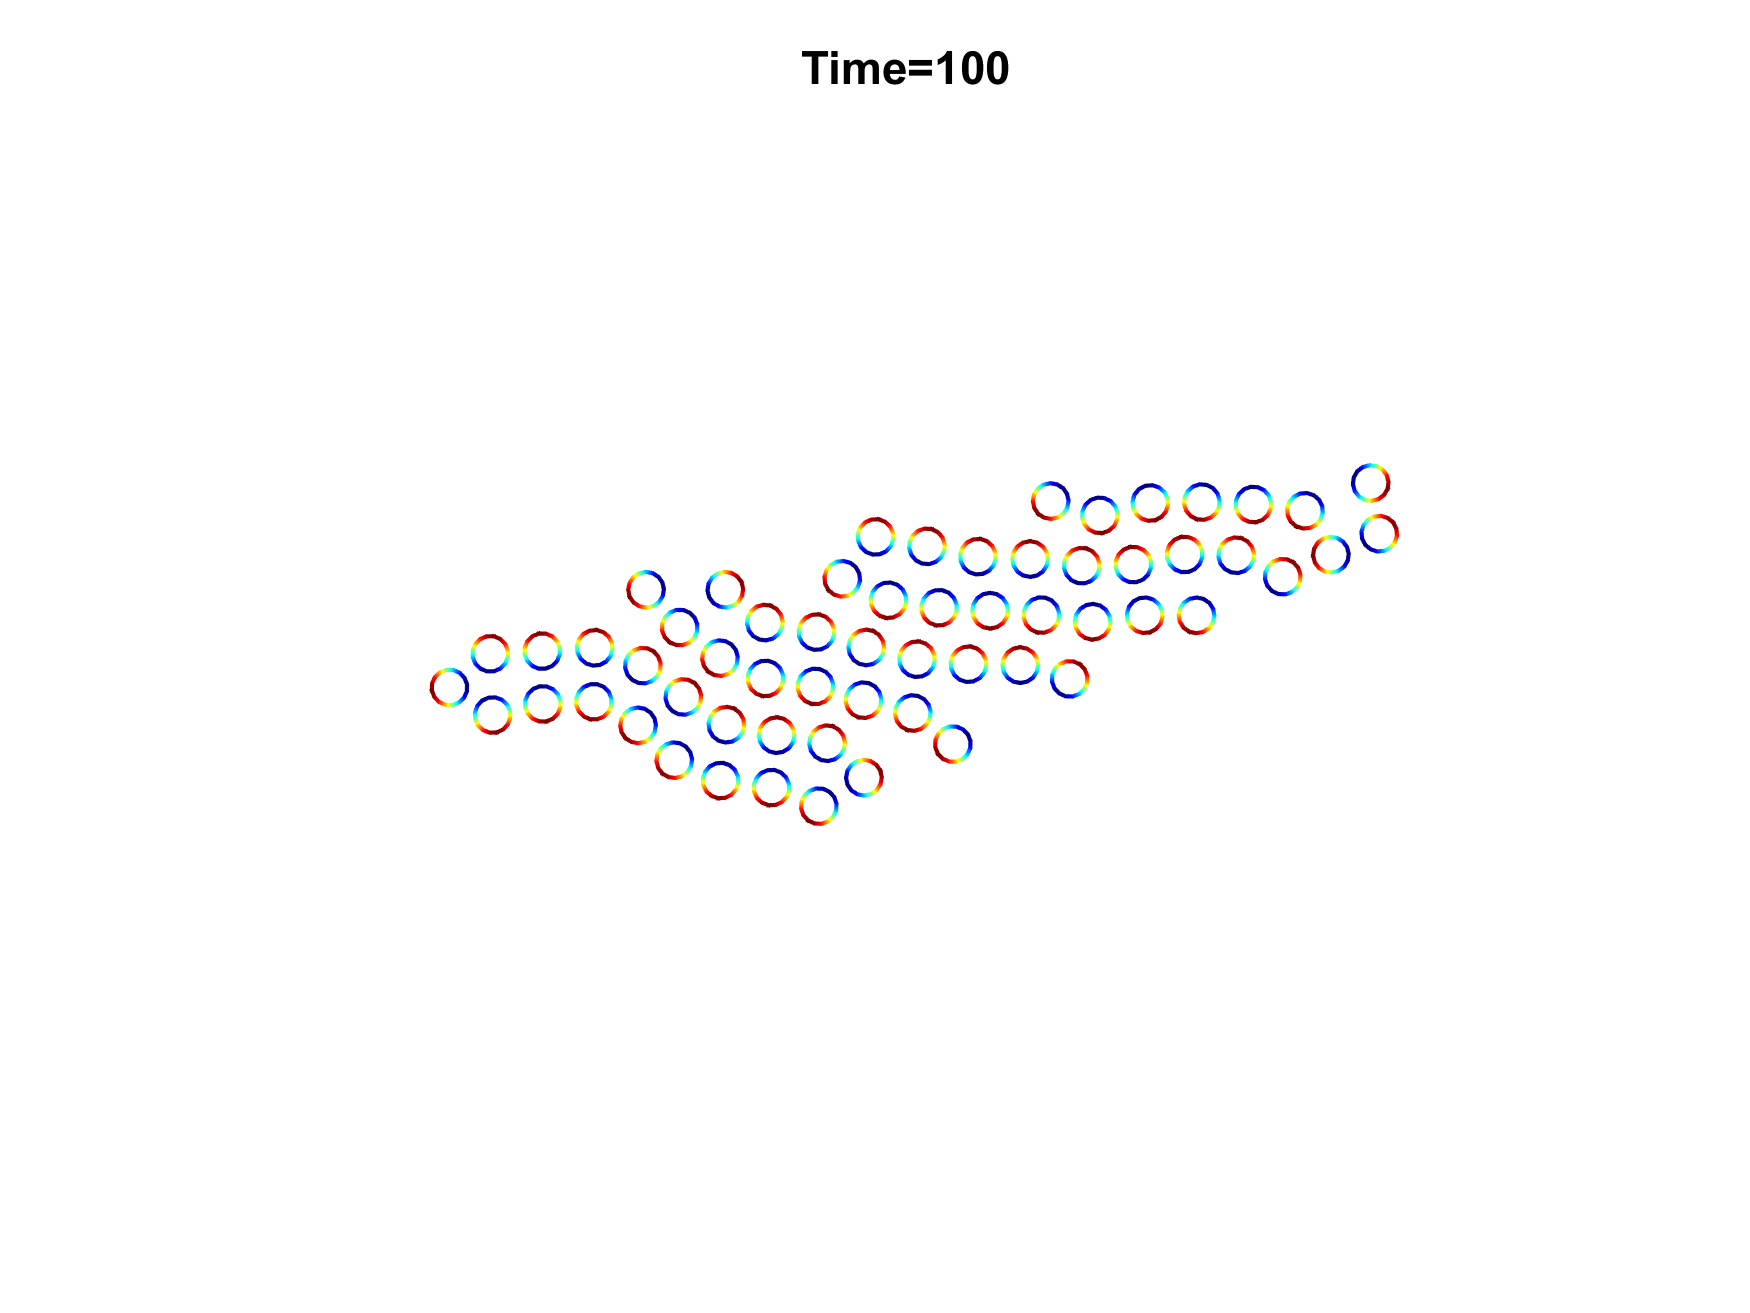
\includegraphics[width=0.4\textwidth]{shear_checker_500.png}
%    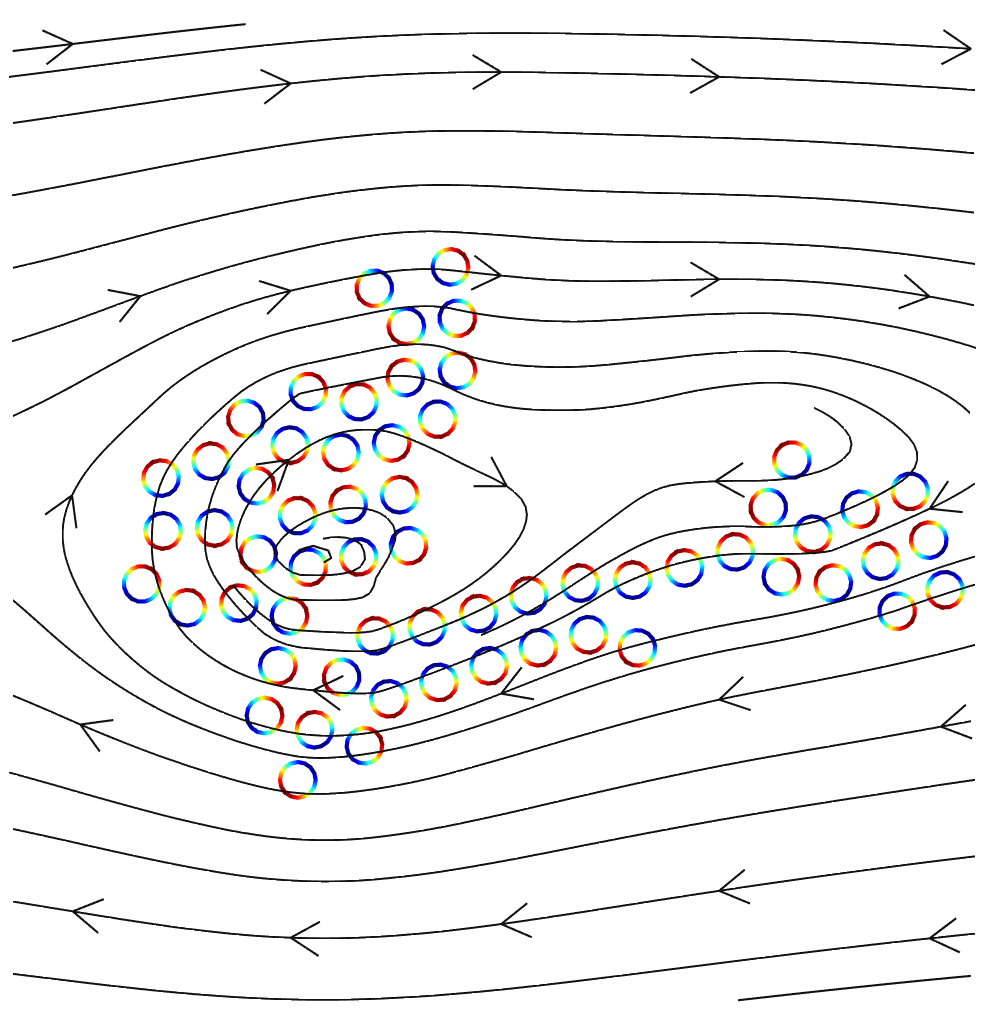
\includegraphics[width=0.4\textwidth]{shear_checker_750.png}
%  \end{center}
%  \vspace{-20pt}  
%  \caption{\label{fig:shear_2} Snapshots of simulation using boundary condition \eqref{eq:bcs}(iii) in a shear flow when $\dot\gamma=0.15$. }
%\end{figure}


\subsection{Collective Janus Particles Suspended in a Taylor-Green Flow}

Similar to shear flow simulations, we then place equilibrium states of all boundary conditions \eqref{eq:bcs} in a rotating Taylor-Green Flow with a length scale $l$,
\begin{equation}
\uu_\infty(\xx) = V_0 \left(-\cos(l{\bf e}_x\cdot\xx)\sin(l{\bf e}_y\cdot\xx){\bf e}_x+\sin(l{\bf e}_x\cdot\xx)\cos(l{\bf e}_y\cdot\xx){\bf e}_y\right).
\end{equation}
%
The magnitude of the vortex flow is controlled by the velocity scale
$V_0$.  Similar to the setup in the shear flow cases, we shift the
center of mass position to the origin then turn on the Taylor-Green flow
with $V_0=0.1$ and tune the sides of zero-velocity box to $\pi$, i.e.,
$l=0.5$, Figure~\ref{fig:TG_1}(a)--(c) show three frames of simulation
results and we track the aspect ratio $\lambda$ described in the
previous section which is provided in panel (d).  The stiffness of the
multilamellar structure is able to compete with the flow therefore the
structure does not deform to any states other than multilamellar shape.
We also found that the flow strength coefficient above $V_0=0.1$ will
result to clear group separations during the simulations.  Comparing
with the case when $V_0=0.2$, we provide a frame in
Figure~\ref{fig:TG_2}(a) and the energy comparison is shown in panel
(b). Numerical results validate the phenomenon that a higher
Taylor-Green vortex flow generates large structure separations with
higher total energy.


\begin{figure}
  \begin{center}
  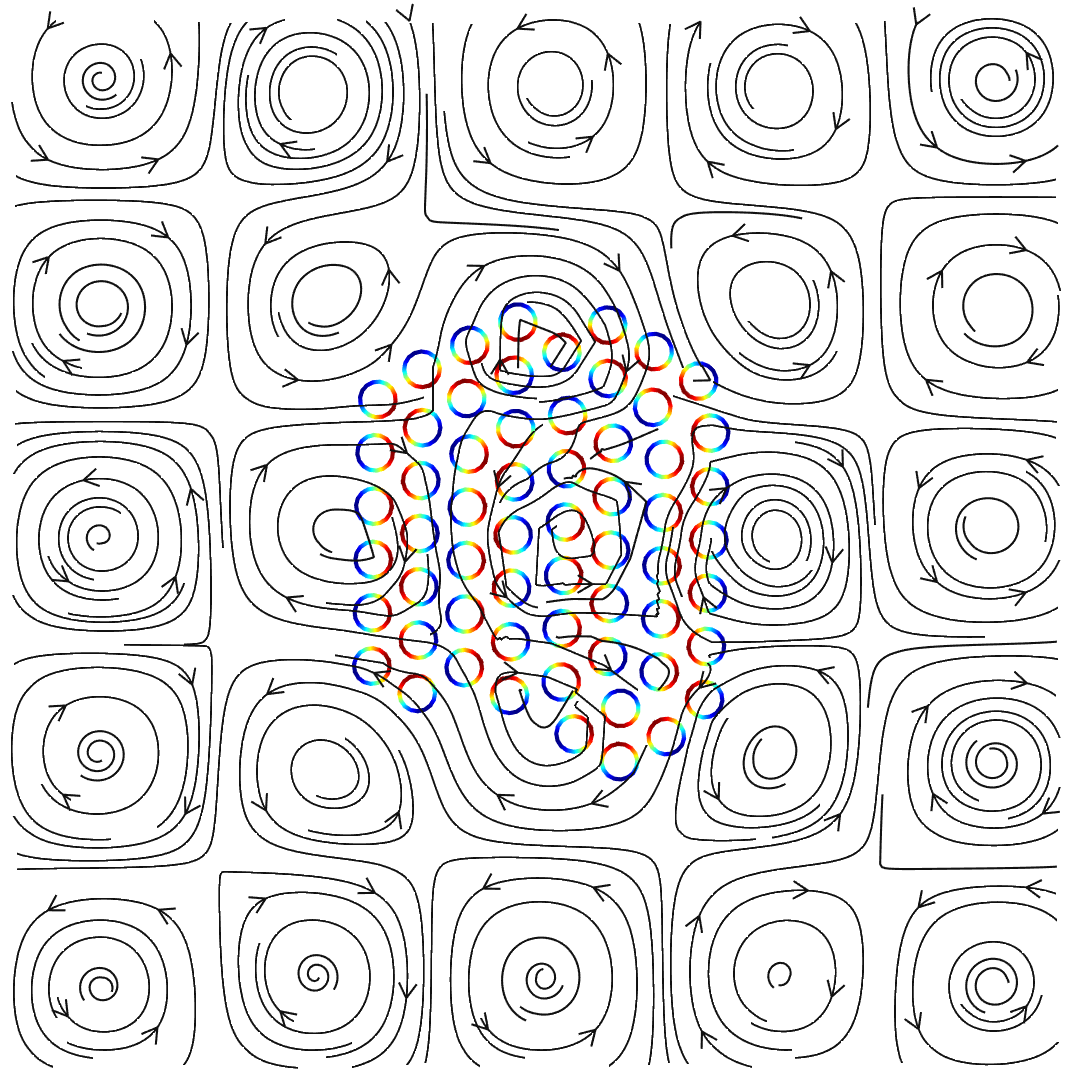
\includegraphics[width=0.4\textwidth]{TG_0.png}
  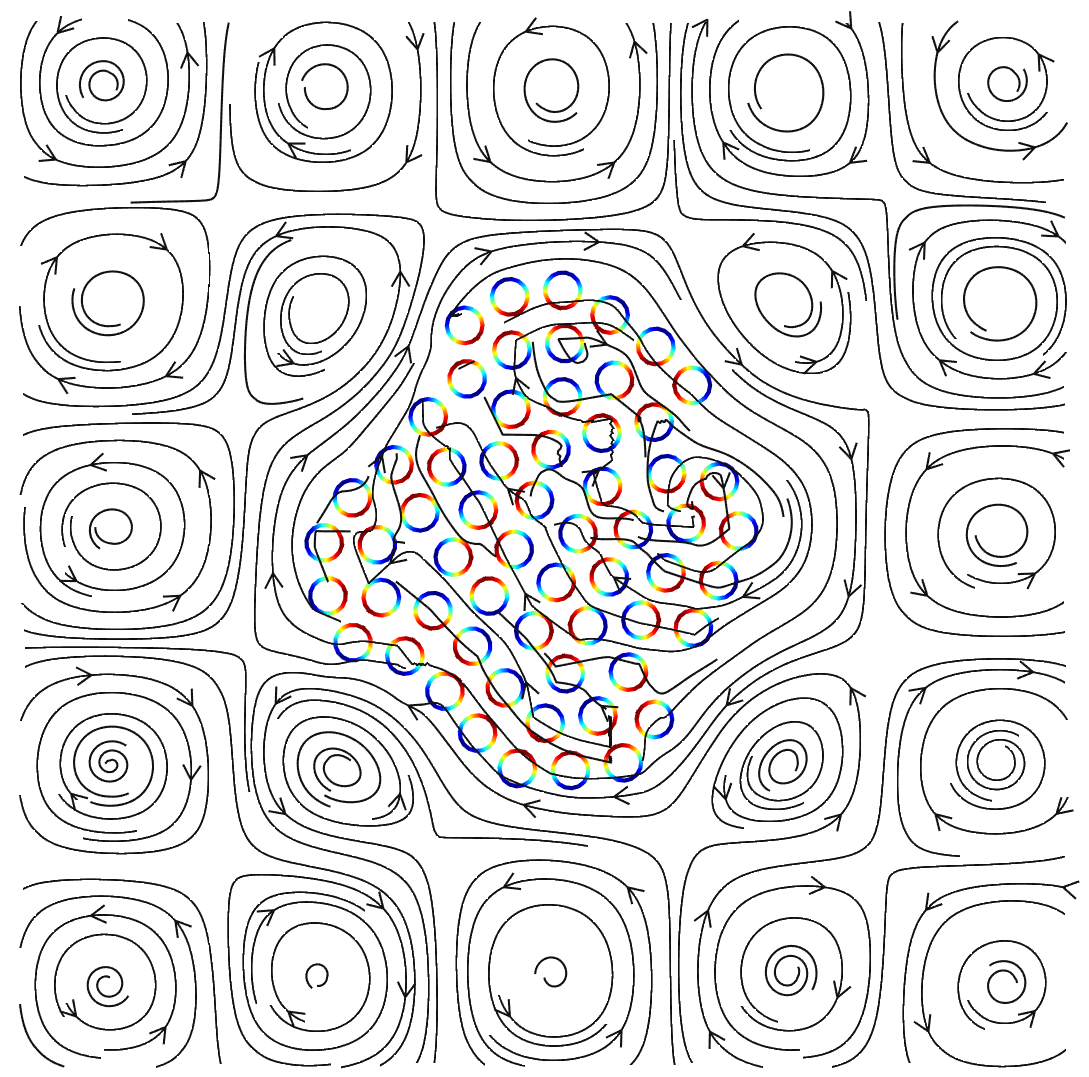
\includegraphics[width=0.4\textwidth]{TG_2500.png}\\
  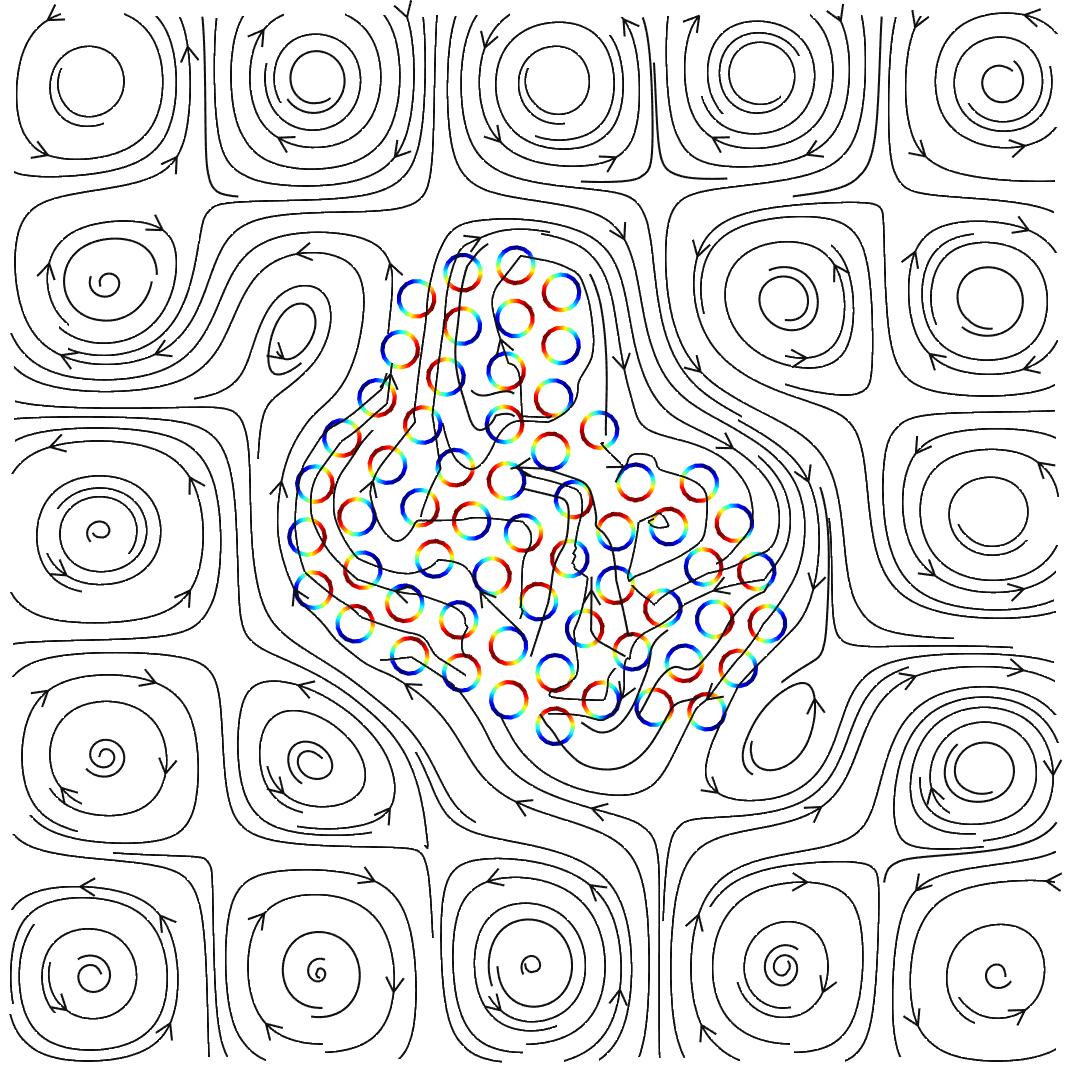
\includegraphics[width=0.4\textwidth]{TG_5000.png}
    \includegraphics[width=0.4\textwidth]{TG_dist.jpg}
  \end{center}
  \vspace{-20pt}  
  \caption{\label{fig:TG_1} Snapshots of simulation using boundary condition \eqref{eq:bcs}(b) in a Taylor-Green flow when $V_0=0.1$ and $l=0.5$.}
\end{figure}


\begin{figure}
  \begin{center}
  \includegraphics[width=0.4\textwidth]{TG0p2_2000.png}
  \includegraphics[width=0.4\textwidth]{TG_energy1.jpg}
  \end{center}
  \vspace{-20pt}  
  \caption{\label{fig:TG_2} (a) Snapshots of simulation using boundary condition \eqref{eq:bcs}(b) in a Taylor-Green flow when $V_0=0.2$, $l=0.5$, and $t = 400$. (b) Energy profiles for two cases $V_0=0.1$ and $V_0=0.2$. }
\end{figure}



\subsection{Steady-State Structure Confined in Narrow Channels}


Here are demonstrations of having JP vesicle and multilamellar
structure in a narrow channel under a shear flow. Simulation results
and snapshots are shown in Figures~\ref{fig:confined_vesicle} and
Figure~\ref{fig:confined_lamellar} where the JP vesicle has $N_b=25$
particles and JP lamellar has $N_b=40$ particles, respectively. Both
starting configurations are pre-relaxed and the channel width in the
narrow part is about 5 length units in the vesicle case and 4 length
units in the lamellar case.


\begin{figure}
  \begin{center}
  \includegraphics[width=0.4\textwidth]{VesConf_0.png}
  \includegraphics[width=0.4\textwidth]{VesConf_2000.png}\\
  \includegraphics[width=0.4\textwidth]{VesConf_5000.png}
  \includegraphics[width=0.4\textwidth]{VesConf_10000.png}
  \end{center}
  \vspace{-20pt}  
  \caption{\label{fig:confined_vesicle} A JP vesicle confined in a narrow channel where $N_b=25$ and $\dot\gamma=0.01$.  }
\end{figure}




\begin{figure}
  \begin{center}
  \includegraphics[width=0.4\textwidth]{MultConf_100.png}
  \includegraphics[width=0.4\textwidth]{MultConf_600.png}\\
  \includegraphics[width=0.4\textwidth]{MultConf_1200.png}
  \includegraphics[width=0.4\textwidth]{MultConf_2400.png}
  \end{center}
  \vspace{-20pt}  
  \caption{\label{fig:confined_lamellar} A JP multilamellar structure
  confined in a narrow channel where $N_b=40$ and $\dot\gamma=0.05$.}
\end{figure}


\section{Conclusions}




%%%

% If in two-column mode, this environment will change to single-column
% format so that long equations can be displayed. Use
% sparingly.
%\begin{widetext}
% put long equation here
%\end{widetext}

% figures should be put into the text as floats.
% Use the graphics or graphicx packages (distributed with LaTeX2e)
% and the \includegraphics macro defined in those packages.
% See the LaTeX Graphics Companion by Michel Goosens, Sebastian Rahtz,
% and Frank Mittelbach for instance.
%
% Here is an example of the general form of a figure:
% Fill in the caption in the braces of the \caption{} command. Put the label
% that you will use with \ref{} command in the braces of the \label{} command.
% Use the figure* environment if the figure should span across the
% entire page. There is no need to do explicit centering.

% \begin{figure}
% \includegraphics{}%
% \caption{\label{}}
% \end{figure}

% Surround figure environment with turnpage environment for landscape
% figure
% \begin{turnpage}
% \begin{figure}
% \includegraphics{}%
% \caption{\label{}}
% \end{figure}
% \end{turnpage}

% tables should appear as floats within the text
%
% Here is an example of the general form of a table:
% Fill in the caption in the braces of the \caption{} command. Put the label
% that you will use with \ref{} command in the braces of the \label{} command.
% Insert the column specifiers (l, r, c, d, etc.) in the empty braces of the
% \begin{tabular}{} command.
% The ruledtabular enviroment adds doubled rules to table and sets a
% reasonable default table settings.
% Use the table* environment to get a full-width table in two-column
% Add \usepackage{longtable} and the longtable (or longtable*}
% environment for nicely formatted long tables. Or use the the [H]
% placement option to break a long table (with less control than 
% in longtable).
% \begin{table}%[H] add [H] placement to break table across pages
% \caption{\label{}}
% \begin{ruledtabular}
% \begin{tabular}{}
% Lines of table here ending with \\
% \end{tabular}
% \end{ruledtabular}
% \end{table}

% Surround table environment with turnpage environment for landscape
% table
% \begin{turnpage}
% \begin{table}
% \caption{\label{}}
% \begin{ruledtabular}
% \begin{tabular}{}
% \end{tabular}
% \end{ruledtabular}
% \end{table}
% \end{turnpage}

% Specify following sections are appendices. Use \appendix* if there
% only one appendix.
%\appendix
%\section{}



